\documentclass[10pt,a4paper,oneside]{report}
\usepackage[margin=2.4cm]{geometry}
\usepackage{amsmath,amssymb}
\usepackage{graphicx}
\usepackage{booktabs}
\usepackage{longtable}
\usepackage{tabularx}
\usepackage{array}
\usepackage{xcolor}
\usepackage{listings}
\usepackage{tikz}
\usetikzlibrary{arrows.meta,positioning,fit,calc,shapes.geometric}
\usepackage{algorithm}
\usepackage{algpseudocode}
\usepackage{enumitem}
\usepackage{fancyhdr}
\usepackage{titlesec}
\usepackage{caption}
\usepackage[hidelinks]{hyperref}

\graphicspath{{../images/}{../results/climate-rescue-2026-10-18/figures/}{../images/trait-snapshot/}{../images/diploid-preview/}}

\definecolor{vk}{HTML}{1F6F5C}
\definecolor{vkl}{HTML}{E8F3EF}
\definecolor{codebg}{HTML}{F5F6F7}
\hypersetup{colorlinks=true,linkcolor=vk,urlcolor=vk,citecolor=vk}

\lstset{basicstyle=\ttfamily\small,backgroundcolor=\color{codebg},frame=single,
  rulecolor=\color{gray!40},breaklines=true,columns=fullflexible,keepspaces=true,
  xleftmargin=4pt,xrightmargin=4pt,aboveskip=6pt,belowskip=6pt}

\titleformat{\chapter}[display]{\normalfont\bfseries\color{vk}\raggedright}{\large Chapter \thechapter}{4pt}{\Huge}
\titlespacing*{\chapter}{0pt}{-10pt}{18pt}
\titleformat{\section}{\normalfont\Large\bfseries\color{vk}}{\thesection}{0.8em}{}

\pagestyle{fancy}
\fancyhf{}
\fancyhead[L]{\small\color{gray}Vikasa Technical Documentation}
\fancyhead[R]{\small\color{gray}\nouppercase{\leftmark}}
\fancyfoot[C]{\thepage}
\renewcommand{\headrulewidth}{0.3pt}
\fancypagestyle{plain}{\fancyhf{}\fancyfoot[C]{\thepage}\renewcommand{\headrulewidth}{0pt}}

\setlength{\parskip}{4pt}
\setlength{\parindent}{0pt}
\newcolumntype{L}{>{\raggedright\arraybackslash}X}
\newcommand{\code}[1]{\texttt{\small #1}}
\newcommand{\note}[1]{\begin{center}\fcolorbox{vk}{vkl}{\parbox{0.92\linewidth}{\small #1}}\end{center}}

% Chapters flow on from the previous one instead of always starting a new page.
\usepackage{etoolbox}
\usepackage{needspace}
\makeatletter
\patchcmd{\chapter}{\if@openright\cleardoublepage\else\clearpage\fi}{\par\needspace{0.3\textheight}\vspace{18pt}}{}{}
\patchcmd{\chapter}{\global\@topnum\z@}{}{}{}
\makeatother
\titlespacing*{\chapter}{0pt}{0pt}{12pt}
\renewcommand{\floatpagefraction}{0.75}
\renewcommand{\topfraction}{0.85}
\renewcommand{\textfraction}{0.12}
\sloppy
\setlength{\emergencystretch}{3em}

\begin{document}

\begin{titlepage}
\centering
\vspace*{1.2cm}

\includegraphics[width=2.6cm]{../../src/evolution_sim/assets/vikasa-biome.png}\par
\vspace{0.8cm}
{\Huge\bfseries\color{vk} Vikasa\par}
\vspace{0.3cm}
{\LARGE Living Biome \& Climate Rescue\par}
\vspace{0.6cm}
{\Large Complete Technical Documentation\par}
\vspace{0.4cm}
{\large Version 2.3\par}
\vspace{1cm}
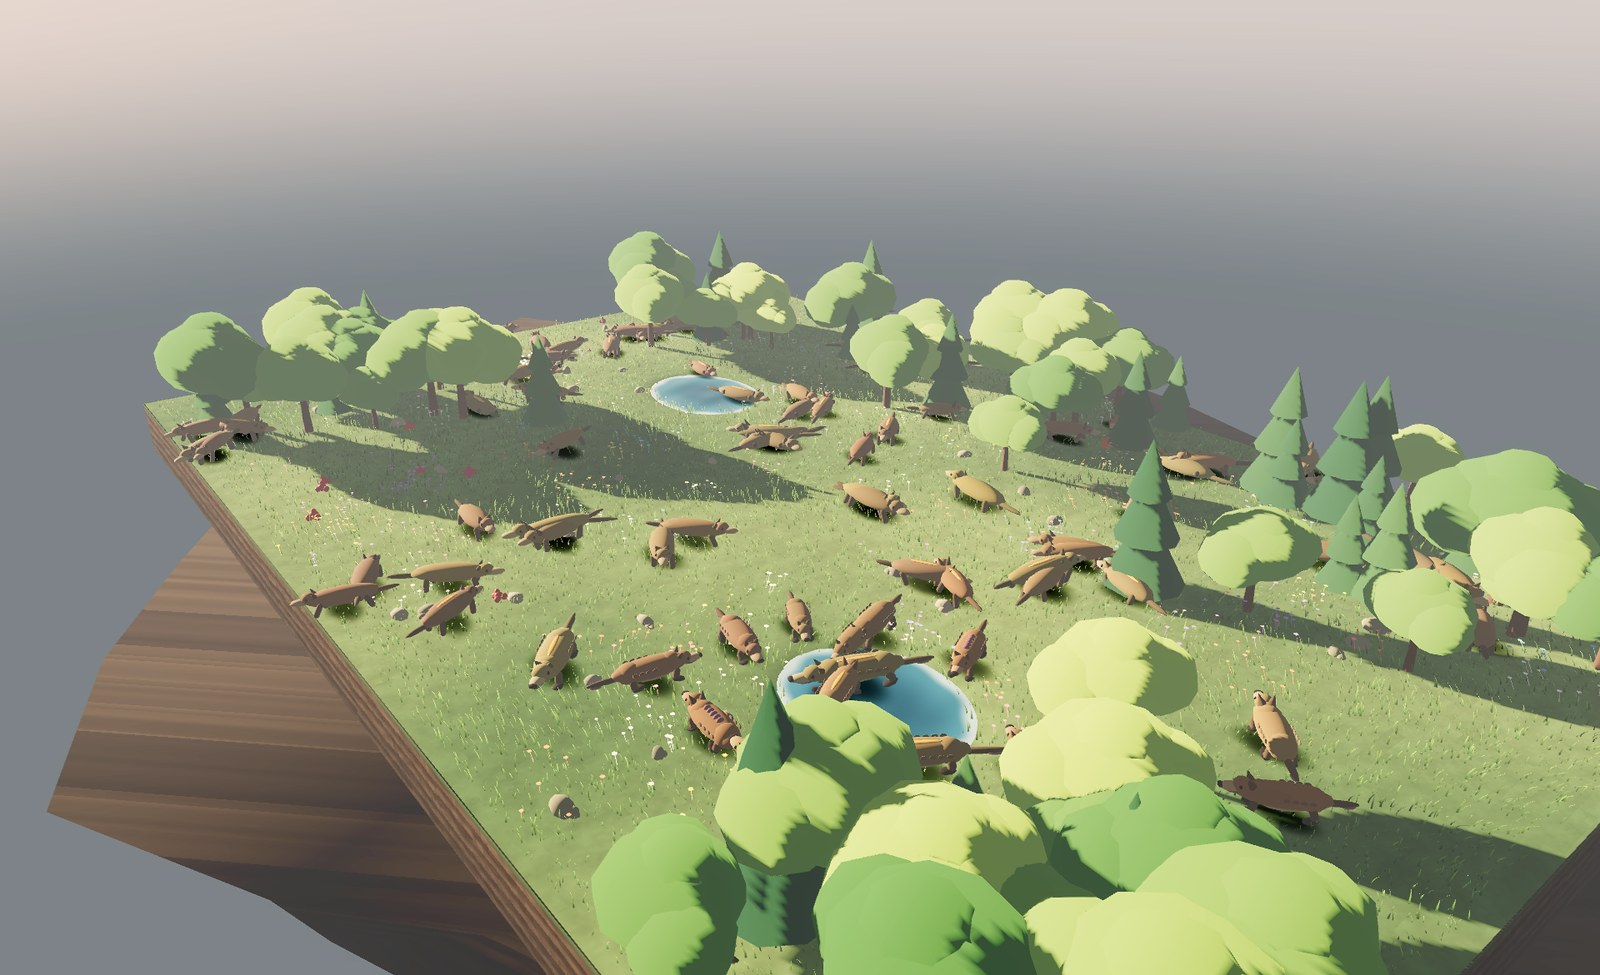
\includegraphics[width=0.92\textwidth]{showcase-hero.jpg}\par
\vspace{1cm}
{\large A deterministic, individual-based evolution simulator with a cinematic 3D
client, real climate data, a Species Risk Checker and a Conservation Planner\par}
\vfill
{\large Sushanth Kasturi\par}
{\small Repository: \url{https://github.com/Linuxboii/vikasa}\quad$\cdot$\quad MIT licence\par}
\end{titlepage}

\pagenumbering{roman}
\chapter*{About this document}
\addcontentsline{toc}{chapter}{About this document}
This document is the complete technical reference for Vikasa 2.3. It is written
for four audiences at once: \emph{users} who want to install and run the software,
\emph{scientists} who need to know exactly what the model computes before
trusting any number it produces, \emph{engineers} who will maintain or extend the
code base, and \emph{decision makers} who want to understand what the Species Risk
Checker and the Conservation Planner can and cannot tell them.

Every equation, coefficient and default in this document was taken from the
executable source code (\code{src/evolution\_sim/}) and the evidence packages
committed under \code{docs/results/}. Where the project's own Markdown guides
contain further detail, the relevant file is named so the reader can follow it.
Measured numbers always carry their provenance: configuration, seeds, horizon and,
where applicable, uncertainty intervals.

\note{\textbf{Scientific scope.} Vikasa is an explanatory artificial-life model.
The climate forcing (NASA POWER temperature records and IPCC AR6 pathways) is
observed data, but the organism is a generic model, not a calibrated real species.
Ticks have no fixed conversion to seconds, days or years. Results are properties
of this model unless explicitly validated otherwise.}

\textbf{Conventions.} Monospaced text denotes code, file paths and commands.
Windows commands are given in PowerShell form (\code{.\textbackslash.venv\textbackslash Scripts\textbackslash vikasa.exe});
on macOS and Linux replace the prefix with \code{.venv/bin/}. The function
$\mathrm{clip}(x)=\min(1,\max(0,x))$ is used throughout. ``Tick'' means one
discrete engine step.

\tableofcontents
\clearpage
\pagenumbering{arabic}

%===========================================================
\chapter{Introduction}
%===========================================================

\section{What Vikasa is}
Vikasa (Sanskrit for ``development'' or ``unfolding'') is a \textbf{deterministic,
individual-based evolution simulator}. Every animal in its world inherits a body
genome and a behavioural temperament, perceives its surroundings, and decides for
itself what to do next. Populations forage, court, fight, raise young, starve,
age and evolve over generations. Nothing on screen is scripted: every birth,
death and clash is the outcome of explicit, inspectable rules evaluated by one
seeded random-number generator.

On top of that core, Vikasa asks a concrete real-world question:

\begin{quote}
\emph{Climate change is not only about how hot it gets, but whether life can adapt
in time. Fast breeders can evolve; slow breeders fall behind. Where is the line?}
\end{quote}

To answer it, Vikasa forces its world with real temperature records (NASA POWER
monthly reanalysis for Indian regions) and IPCC AR6 warming pathways, gives every
animal a heritable thermal optimum, and measures the \emph{critical rate} of
warming beyond which evolution can no longer keep a population alive. The answer,
$0.262\,^{\circ}$C per generation with inheritance against $0.067\,^{\circ}$C per
generation without, is then turned into two practical tools: the \textbf{Species
Risk Checker} and the \textbf{Conservation Planner}.

\section{The project at a glance}

\begin{table}[htbp]
\centering
\caption{Vikasa 2.3 at a glance}
\begin{tabularx}{\textwidth}{lL}
\toprule
\textbf{The question} & Can a population evolve fast enough to survive warming, and how fast is too fast? \\
\textbf{The answer} & With heritable heat tolerance a population survives warming up to 0.262\,$^{\circ}$C per generation, about 4$\times$ more than without inheritance. Under SSP5-8.5, species with generations longer than about 6 years fall behind. \\
\textbf{The tool} & Species Risk Checker: pick a place, describe a species, choose a future, and get an instant estimate, a live simulation and a 3D replay. \\
\textbf{The plan} & Conservation Planner: give it a watchlist and get, per species, the year breeding fails, the heat-tolerance boost that would save it, climate refuges and a ranked action list. \\
\textbf{The showcase} & Demo mode: a presenter hub with a talk timer, one-click launches and a narrated 3D autopilot. \\
\bottomrule
\end{tabularx}
\end{table}

\section{Version history}
Vikasa evolved through clearly separated releases. Knowing which release produced
which evidence matters, because changed coefficients change trajectories even for
the same seed.

\begin{table}[htbp]
\centering
\caption{Release history}
\begin{tabularx}{\textwidth}{lL}
\toprule
Version & Main additions \\
\midrule
1.0--1.1 & Deterministic engine, six-gene genome, Pygame laboratory, headless CLI, checkpoints, first Godot client with Observatory charts and wildlife behaviour (drives, utilities, home ranges, care, fights, culture). \\
Research upgrade & Gompertz mortality, generational development tracking, exact birth-cohort Price decomposition, trait geometry (PCA) exports, optional spatial plant/water ecology, controlled seed-blocked experiment laboratory, opt-in diploid preview. \\
2.0 & \emph{Living Biome}: GPU-instanced 3D wildlife at a locked 60 FPS on integrated graphics, binary push stream, director camera, lenses, day/night, visible weather, procedural soundscape, adaptive quality. \\
2.1 & Climate rescue: NASA POWER data, IPCC AR6 pathways, heritable thermal optimum, critical-rate sweep, Sobol sensitivity, Gaussian-process surrogate, offline report. \\
2.2 & Species Risk Checker, Demo mode with presenter hub and 3D autopilot, one-app home screen and a single desktop shortcut. \\
2.3 & Conservation Planner: watchlist triage, breeding-failure years, assisted gene-flow sizing, refuge search, 14 new survey sites (24 total). \\
\bottomrule
\end{tabularx}
\end{table}

\section{Design principles}
Five principles recur across the code base and explain many design decisions
documented later.
\begin{enumerate}[leftmargin=*]
\item \textbf{The engine is authoritative.} One Python \code{SimulationEngine}
owns all state. Renderers, charts and web apps observe snapshots or issue explicit
commands; none decide outcomes.
\item \textbf{Determinism.} One NumPy PCG64 generator, stable integer IDs for
ordering and tie-breaking, and seeded schedules mean the same configuration and
seed reproduce the same world on the same platform.
\item \textbf{Honest evidence.} Extinct and failed runs are retained, uncertainty
is reported with intervals, missing data stays missing (never plotted as zero),
and pre-registered criteria that failed are published as failures.
\item \textbf{Inspectability.} Every animal exposes its current action, the
reason for it and the utility of each alternative. Every evidence package carries
configuration and source hashes and a SHA-256 manifest.
\item \textbf{Presentability.} The same science is delivered through a 3D
showcase that runs smoothly on an ordinary laptop, so non-specialists can see
what the numbers mean.
\end{enumerate}

\section{Code base size}
Vikasa 2.3 contains about 12{,}100 lines of Python in \code{src/} and 6{,}200 lines
of Python tests, about 5{,}700 lines of GDScript and GPU shader code in
\code{godot/}, and 554 collected automated tests (395 test functions, many of them
parametrised), plus nine headless Godot smoke and capture scripts.

%===========================================================
\chapter{Installation and Quick Start}
%===========================================================

\section{Requirements}
\begin{itemize}[leftmargin=*]
\item Python 3.12 or newer.
\item Runtime dependencies (installed automatically): NumPy $\ge$ 2.1, pandas
$\ge$ 2.2, Matplotlib $\ge$ 3.9, pygame-ce $\ge$ 2.5, scikit-learn $\ge$ 1.5, SciPy $\ge$ 1.14.
\item Development extras: pytest, pytest-cov, Hypothesis and Ruff
(\code{pip install -e .[dev]}).
\item Godot 4 for the 3D Living Biome, on a graphics-capable desktop
(Windows, macOS or Linux). No mobile build is provided.
\end{itemize}
The package is built with Hatchling and exposes one console entry point,
\code{vikasa = evolution\_sim.cli:main}.

\section{Windows}
\begin{lstlisting}
winget install --id GodotEngine.GodotEngine --exact --scope user
py -3.12 -m venv .venv
.\.venv\Scripts\python.exe -m pip install --upgrade pip
.\.venv\Scripts\python.exe -m pip install -e .
.\.venv\Scripts\vikasa.exe shortcut      # one "Vikasa" desktop shortcut
.\.venv\Scripts\vikasa.exe app           # open the Vikasa home screen
\end{lstlisting}
The launcher automatically detects a per-user WinGet Godot installation. If Godot
lives elsewhere, pass \code{--godot-path} or set the environment variable
\code{VIKASA\_GODOT\_BINARY}.

\section{macOS}
\begin{lstlisting}
brew install python@3.12
brew install --cask godot
python3.12 -m venv .venv
source .venv/bin/activate
python -m pip install --upgrade pip
python -m pip install -e .
vikasa godot --config config/showcase.json --seed 2026 \
  --godot-path /Applications/Godot.app/Contents/MacOS/Godot
\end{lstlisting}

\section{Linux (Ubuntu 24.04+)}
On Linux the bridge and the client run in two terminals.
\begin{lstlisting}
sudo apt update
sudo apt install -y python3.12 python3.12-venv flatpak
flatpak remote-add --user --if-not-exists flathub \
  https://flathub.org/repo/flathub.flatpakrepo
flatpak install --user -y flathub org.godotengine.Godot
python3.12 -m venv .venv && source .venv/bin/activate
python -m pip install -e .
# Terminal 1
vikasa serve --config config/showcase.json --seed 2026
# Terminal 2
flatpak run org.godotengine.Godot --path "$PWD/godot"
\end{lstlisting}

\section{The desktop shortcut}
\code{vikasa shortcut} writes a single \emph{Vikasa} shortcut that opens the home
screen through \code{pythonw.exe}, so no console window appears. Re-running it
replaces older Vikasa shortcuts, including ones that went straight into the 3D
biome. Optional direct shortcuts are available with \code{--only biome},
\code{--only demo} or \code{--only risk}; \code{--name} and \code{--desktop}
change the shortcut name and location.

\note{\textbf{Troubleshooting a shortcut that does nothing.} Run
\code{vikasa shortcut} from a normal terminal, not from inside a sandboxed agent.
A sandbox can hide the project files from Windows while the shortcut is saved, and
Windows then stores an empty target. Check the target with
\code{(New-Object -ComObject WScript.Shell).CreateShortcut(...).TargetPath}; it
must print the path to \code{.venv\textbackslash Scripts\textbackslash pythonw.exe}.}

\section{First run checklist}
\begin{enumerate}[leftmargin=*]
\item \code{vikasa validate --config config\textbackslash showcase.json} confirms the configuration parses.
\item \code{vikasa app} opens the home screen in the browser on \code{http://127.0.0.1:8787}.
\item Click \emph{Living Biome}. The bridge starts, Godot opens, and 64 founders appear.
\item Press \textbf{F1} in the 3D client for the field guide listing every shortcut.
\item Press \textbf{G} for the Observatory graphs and click any animal to see why it acts.
\end{enumerate}

%===========================================================
\chapter{Feature Tour}
%===========================================================

\section{The home screen}
\begin{figure}[htbp]
\centering
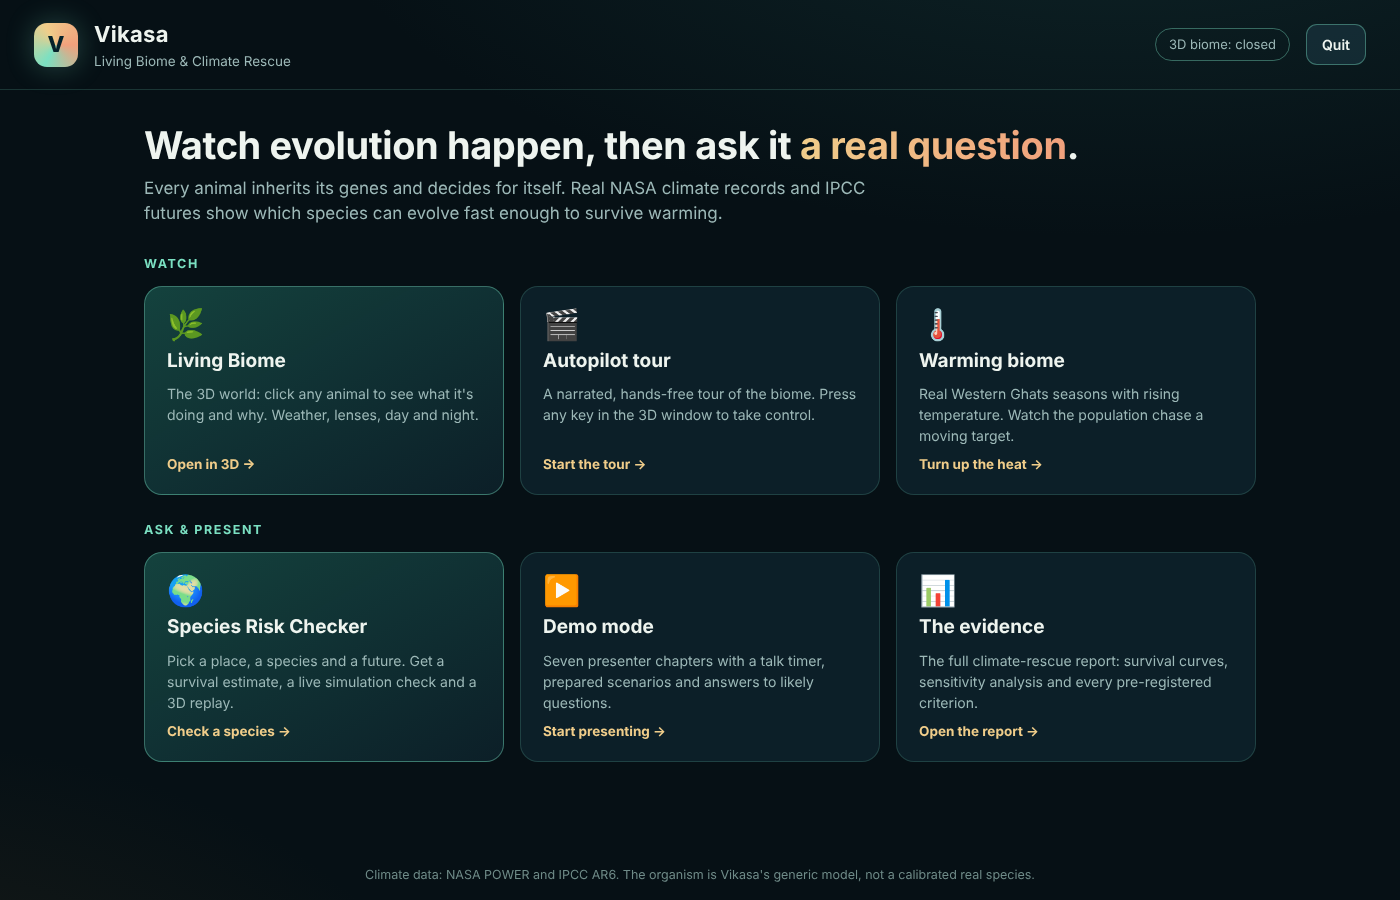
\includegraphics[width=0.85\textwidth]{vikasa-home.png}
\caption{The Vikasa home screen launches every feature with one click.}
\end{figure}
The home screen is served by the local application server on port 8787. It shows
whether a 3D window is open, can close it, and has a \emph{Quit} button that
shuts every Vikasa process down. Only one Vikasa runs per port; an older running
copy is replaced automatically.

\begin{table}[htbp]
\centering
\caption{Home-screen tiles}
\begin{tabularx}{\textwidth}{lL}
\toprule
Tile & What it opens \\
\midrule
Living Biome & The 3D world on the showcase configuration. \\
Autopilot tour & The narrated, hands-free 3D director's cut. \\
Warming biome & The 3D world with real Western Ghats seasons and rising temperature. \\
Species Risk Checker & The browser app for one place and one species (Chapter~\ref{ch:risk}). \\
Demo mode & The seven-chapter presenter hub. \\
The evidence & The committed climate-rescue report. \\
Conservation Planner & Watchlist to rescue plan (Chapter~\ref{ch:planner}). \\
\bottomrule
\end{tabularx}
\end{table}

\section{The Living Biome}
The 3D client renders the whole population with GPU instancing and lets the user
watch it like a nature film. Its main tools:
\begin{itemize}[leftmargin=*]
\item \textbf{Director (C)}: an autonomous camera that finds clashes, newborns,
alphas and families and captions them with letterbox lower-thirds. It only quotes
an explanation when it matches the action on screen.
\item \textbf{Lenses (V)}: recolour animals by coat, action, energy, dynasty
(maternal line), generation depth or temperament; the radar follows the lens.
\item \textbf{Daylight (N)}: cycle, day, golden hour and night, with eyeshine,
fireflies and glowing food after dark (presentation only).
\item \textbf{Legends (L)}: the living elder, most prolific parent, champion,
deepest descendant, best forager and largest dynasty; click to fly there.
\item \textbf{Photo (P)} and \textbf{F12} screenshots to \code{Pictures/Vikasa}.
\item \textbf{World tools (T)}: apply drought, heat, storm, wildfire, cold,
disease, a food-growth bloom, or click to scatter ten audited food patches.
\end{itemize}

\begin{figure}[htbp]
\centering
\begin{minipage}{0.49\textwidth}\centering
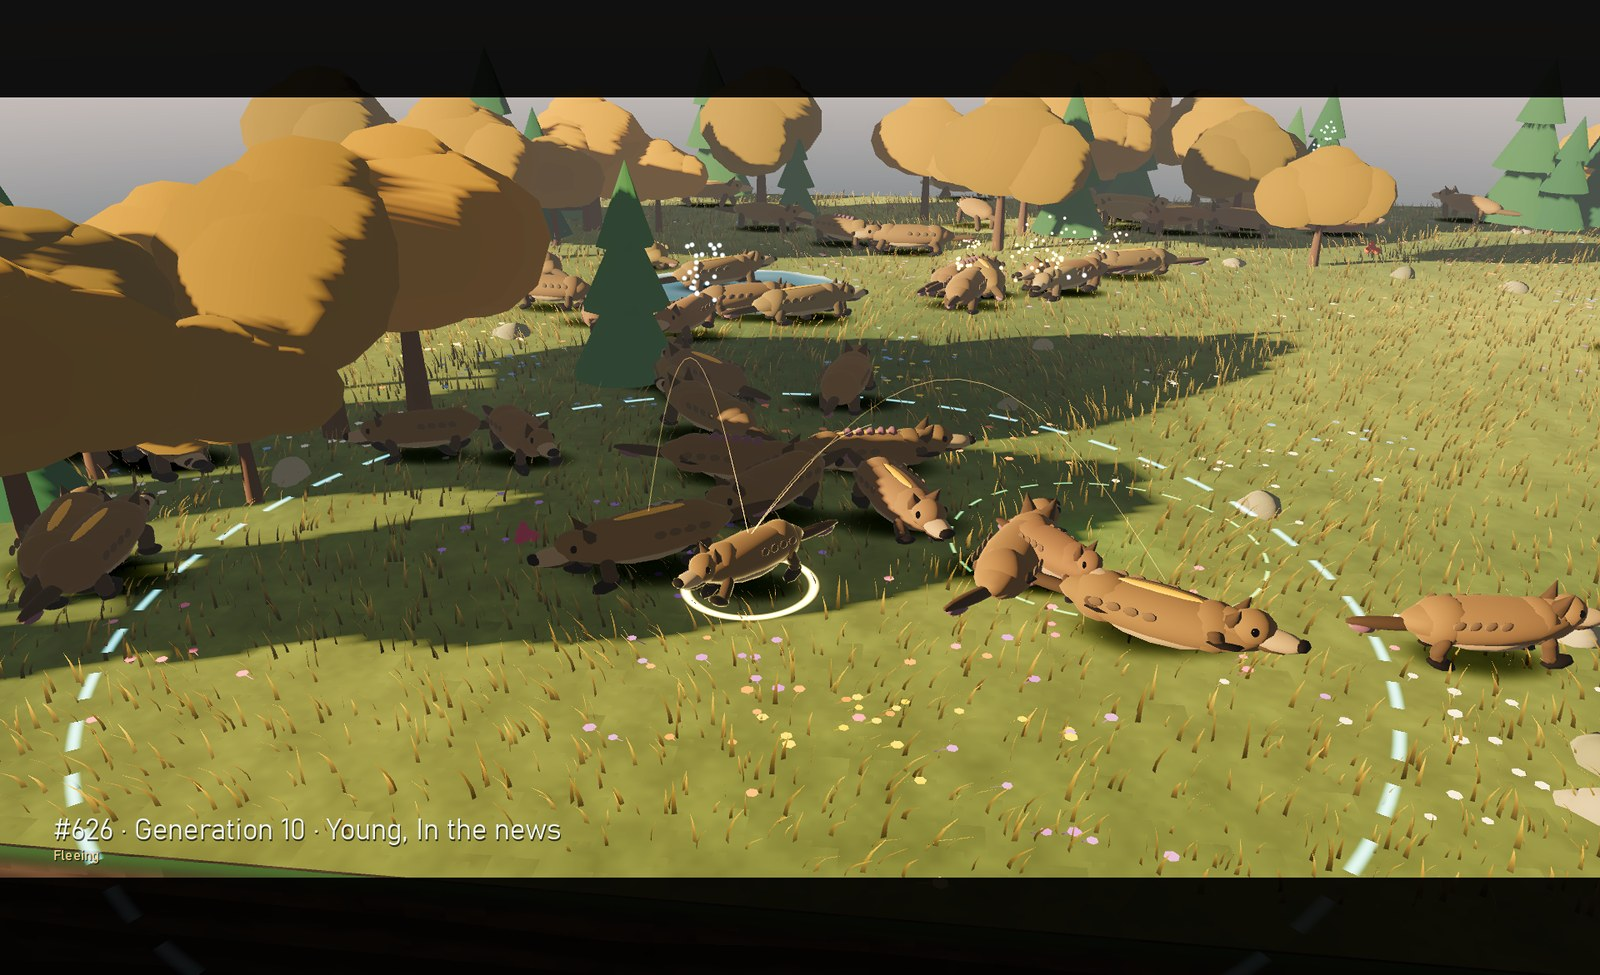
\includegraphics[width=\linewidth]{showcase-director.jpg}\\[-2pt]
{\small (a) Director's cut}
\end{minipage}\hfill
\begin{minipage}{0.49\textwidth}\centering
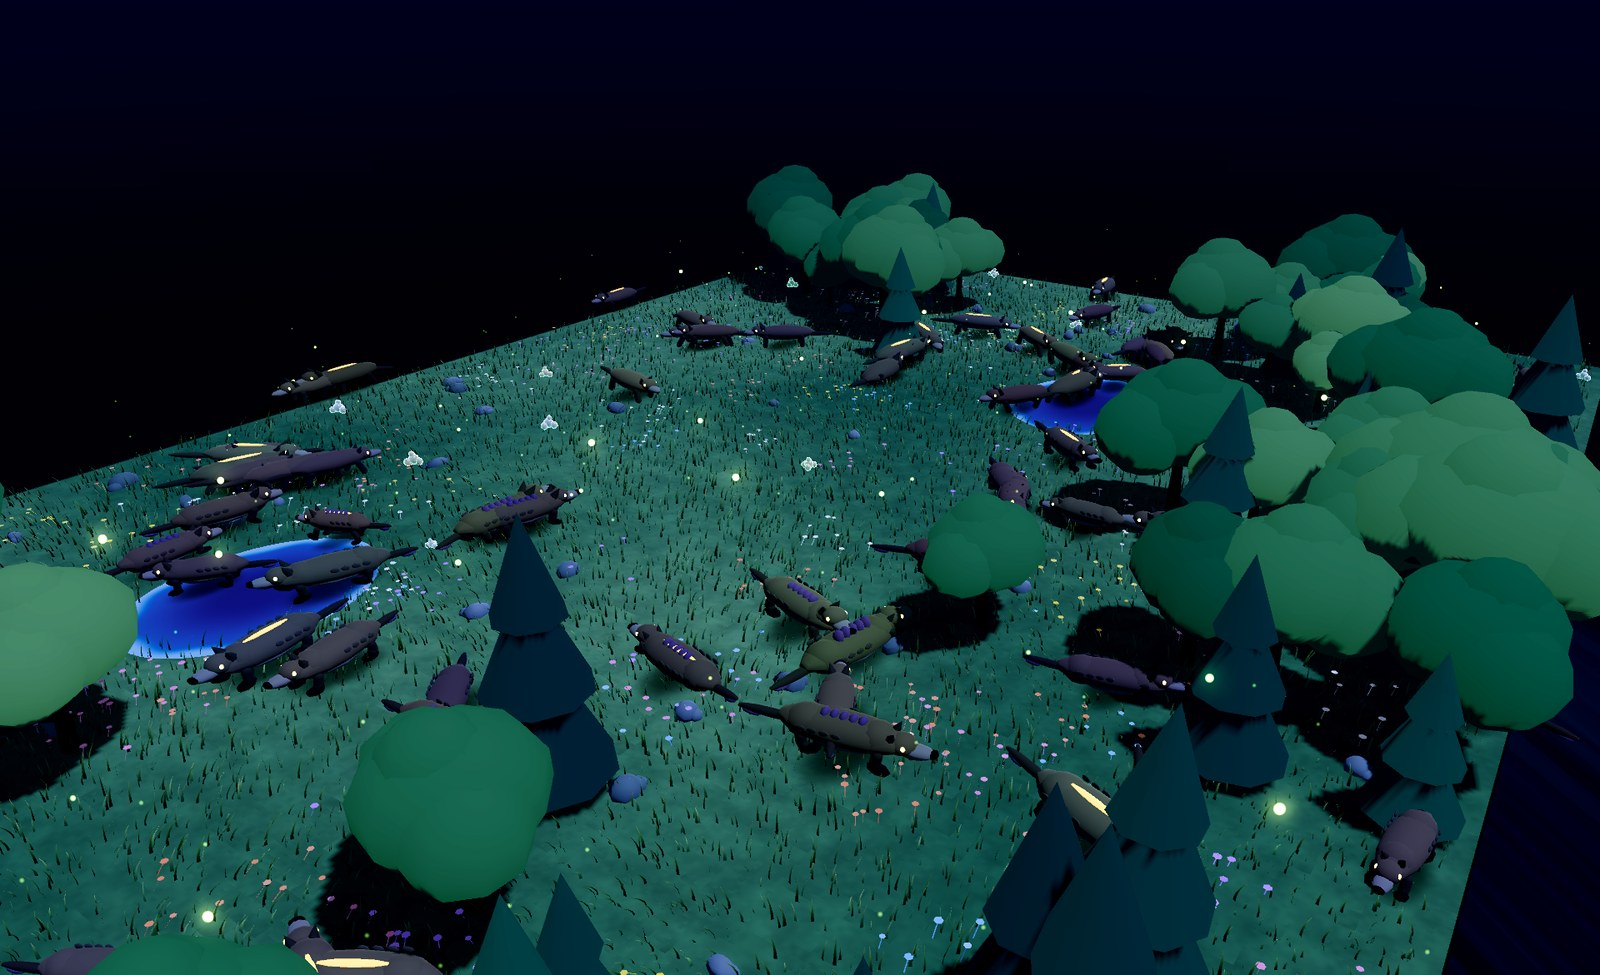
\includegraphics[width=\linewidth]{showcase-night.jpg}\\[-2pt]
{\small (b) Night with eyeshine and fireflies}
\end{minipage}\\[6pt]
\begin{minipage}{0.49\textwidth}\centering
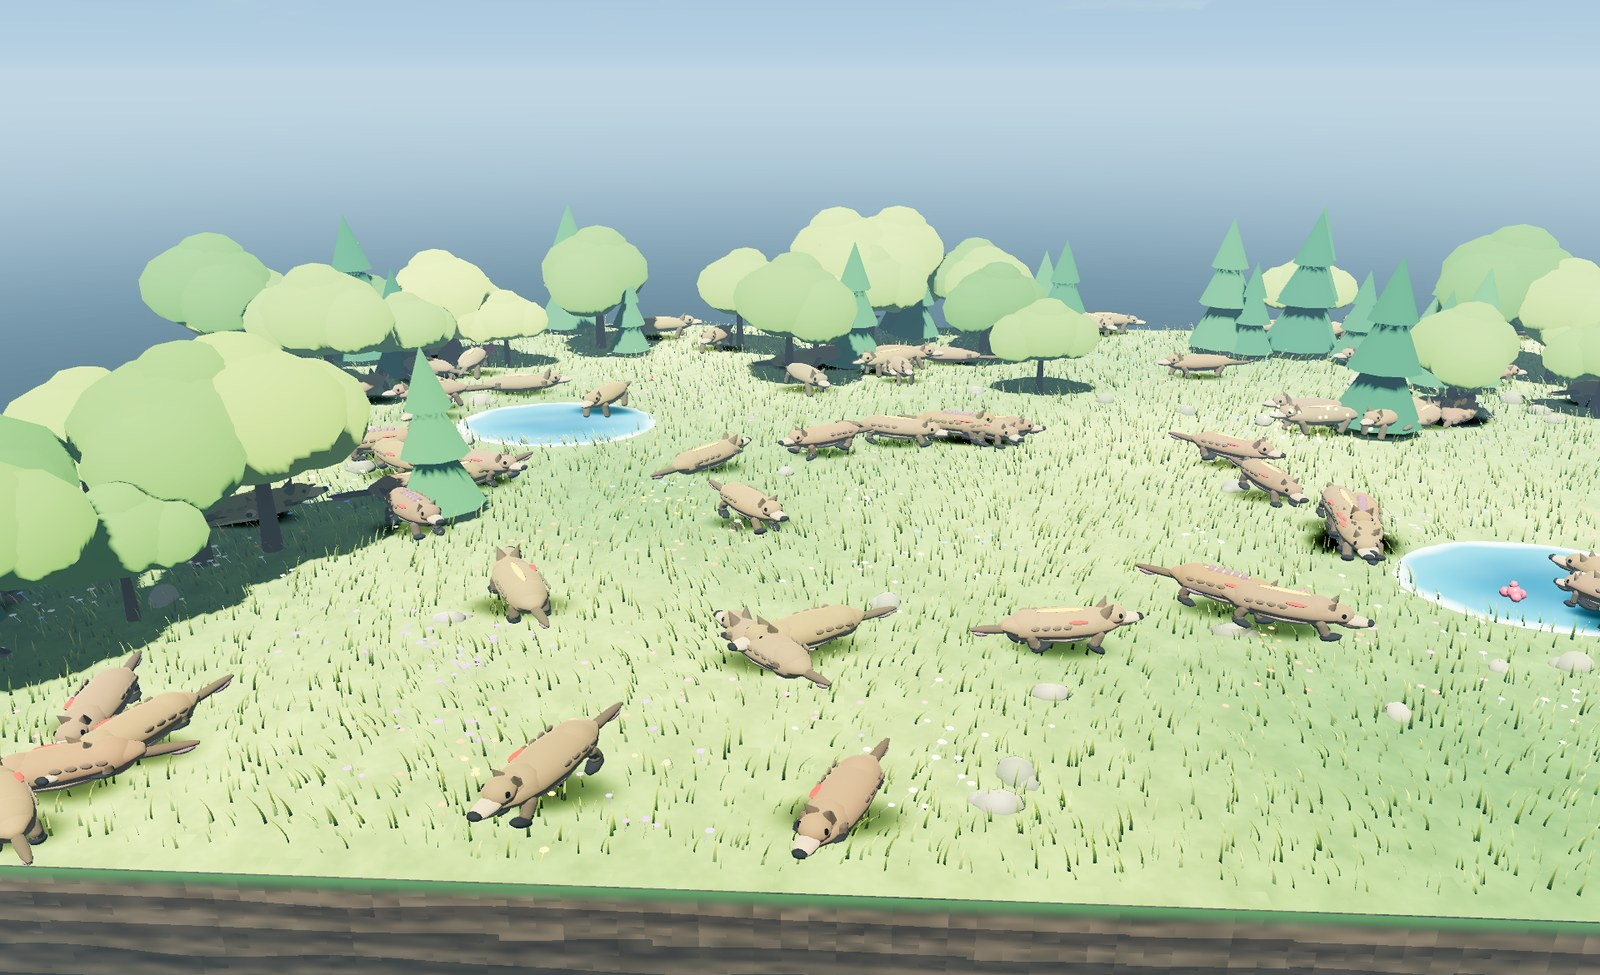
\includegraphics[width=\linewidth]{showcase-storm.jpg}\\[-2pt]
{\small (c) Visible storm}
\end{minipage}\hfill
\begin{minipage}{0.49\textwidth}\centering
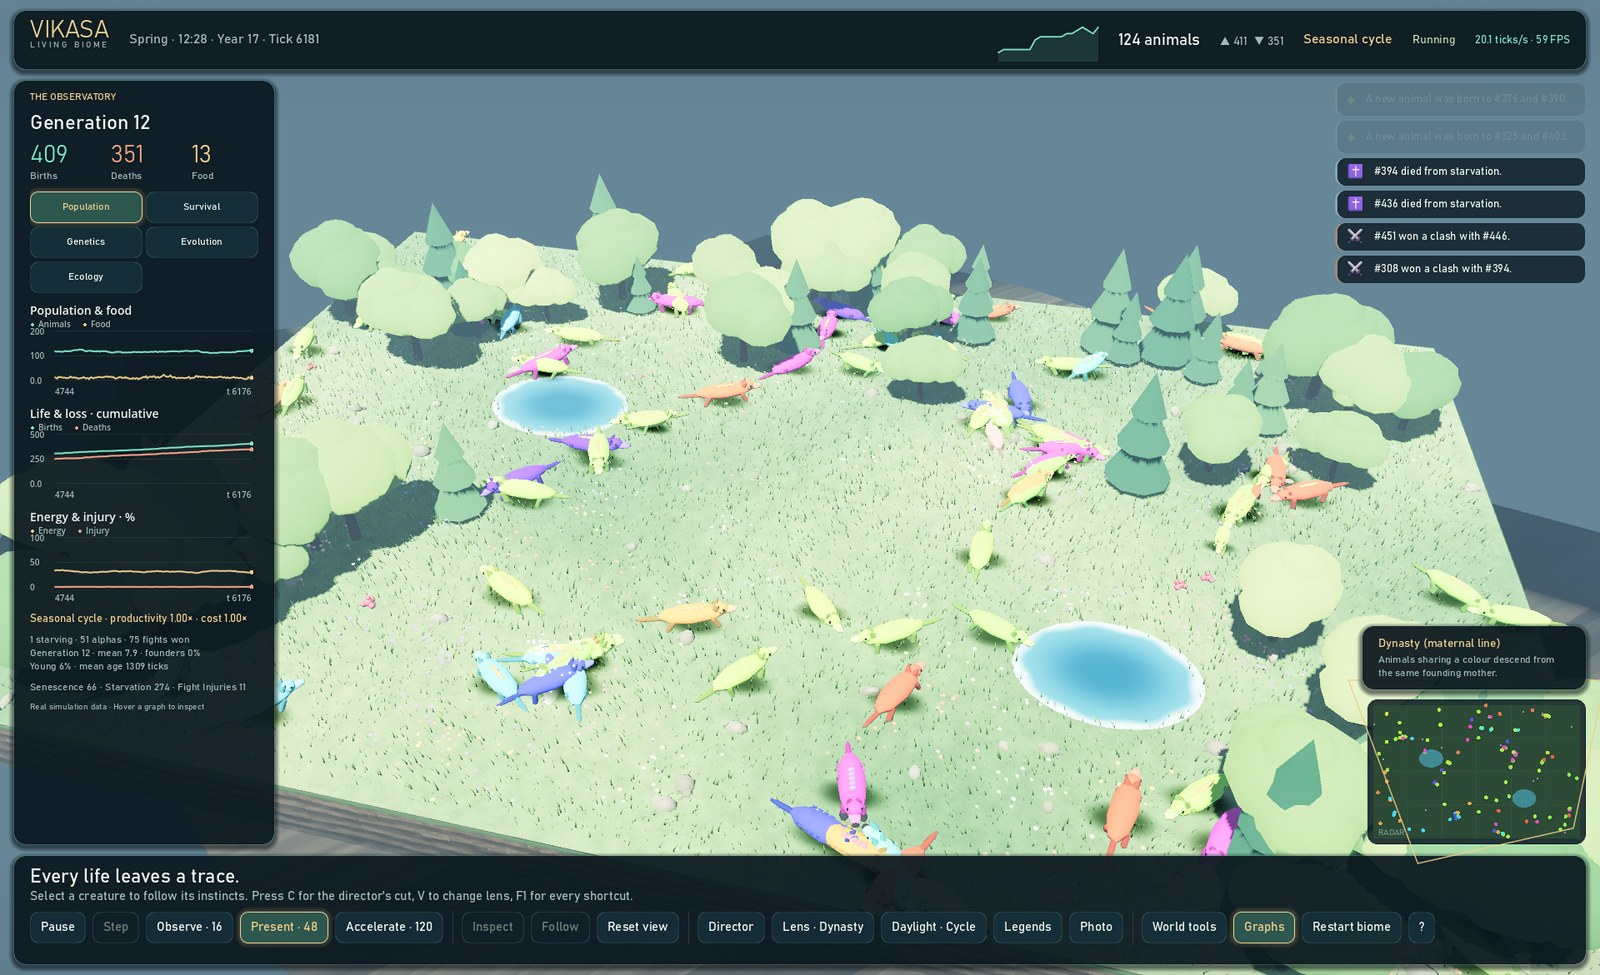
\includegraphics[width=\linewidth]{showcase-lens-dynasty.jpg}\\[-2pt]
{\small (d) Dynasty lens with radar}
\end{minipage}
\caption{Living Biome presentation modes. All captures are real seeded bridge states.}
\end{figure}

\begin{figure}[htbp]
\centering
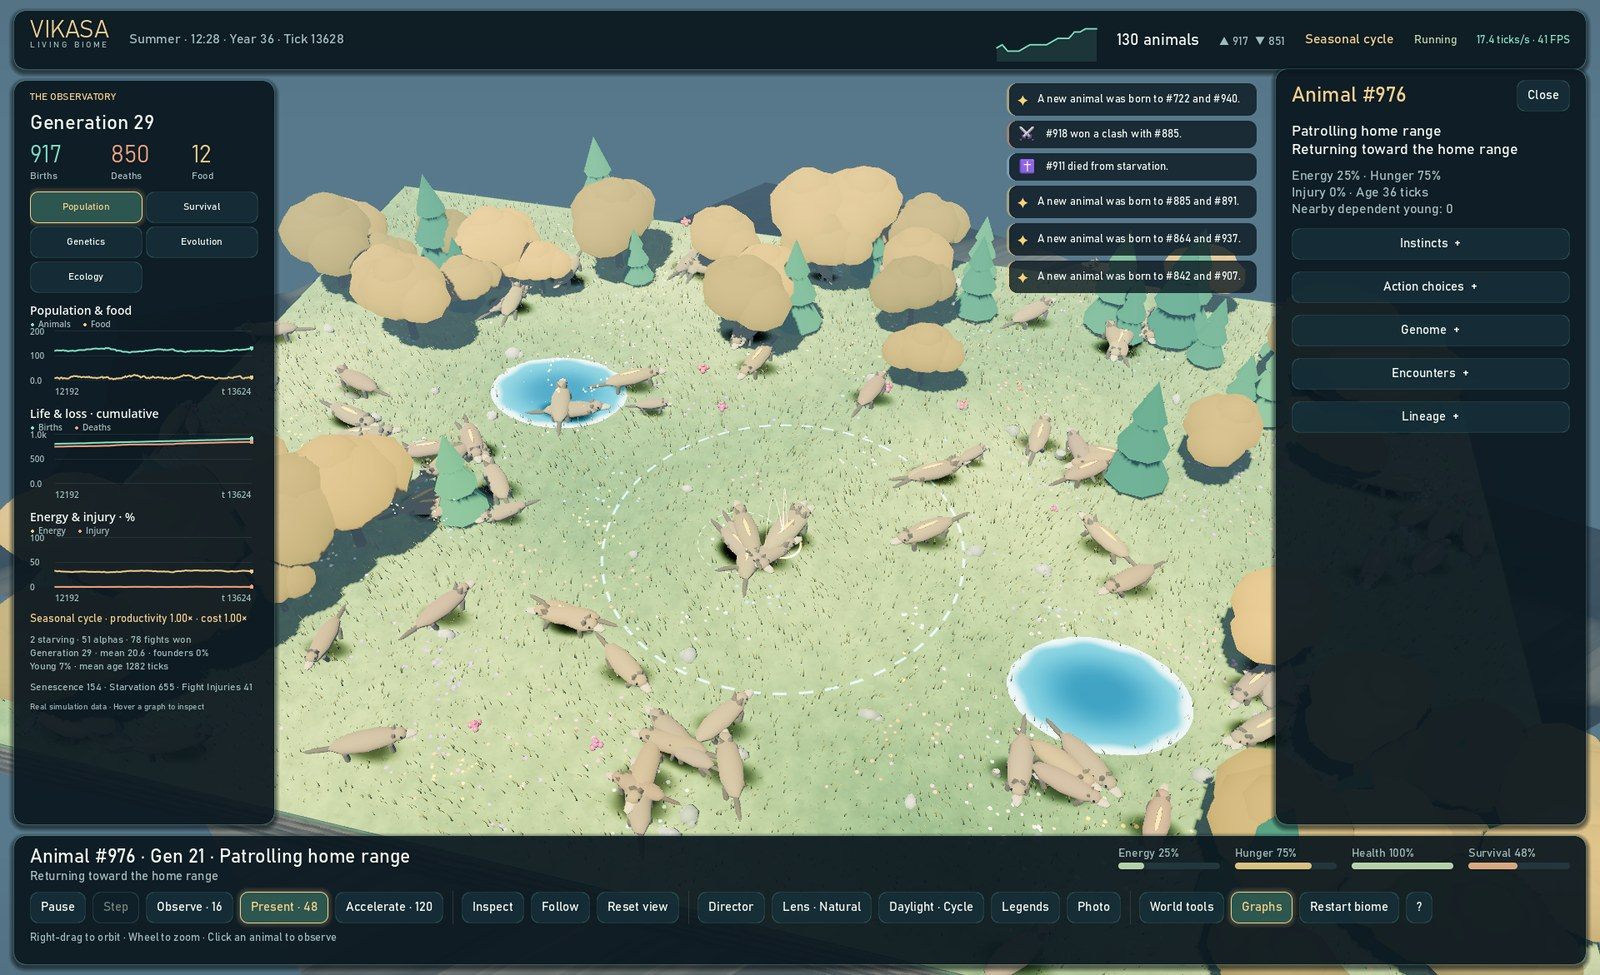
\includegraphics[width=0.95\textwidth]{showcase-interface.jpg}
\caption{Full interface: inspector, event feed, radar minimap and Observatory.}
\end{figure}

Clicking a creature opens its profile: current action and reason, energy, hunger,
injury, instincts (the six drives), top action choices with utilities, genes,
encounters, satisfaction and lineage. In the world, a halo, sensing radius, home
range, a line to the current target and threads to living parents and dependent
young appear (Fig.~\ref{fig:closeup}).

\begin{figure}[htbp]
\centering
\begin{minipage}{0.49\textwidth}\centering
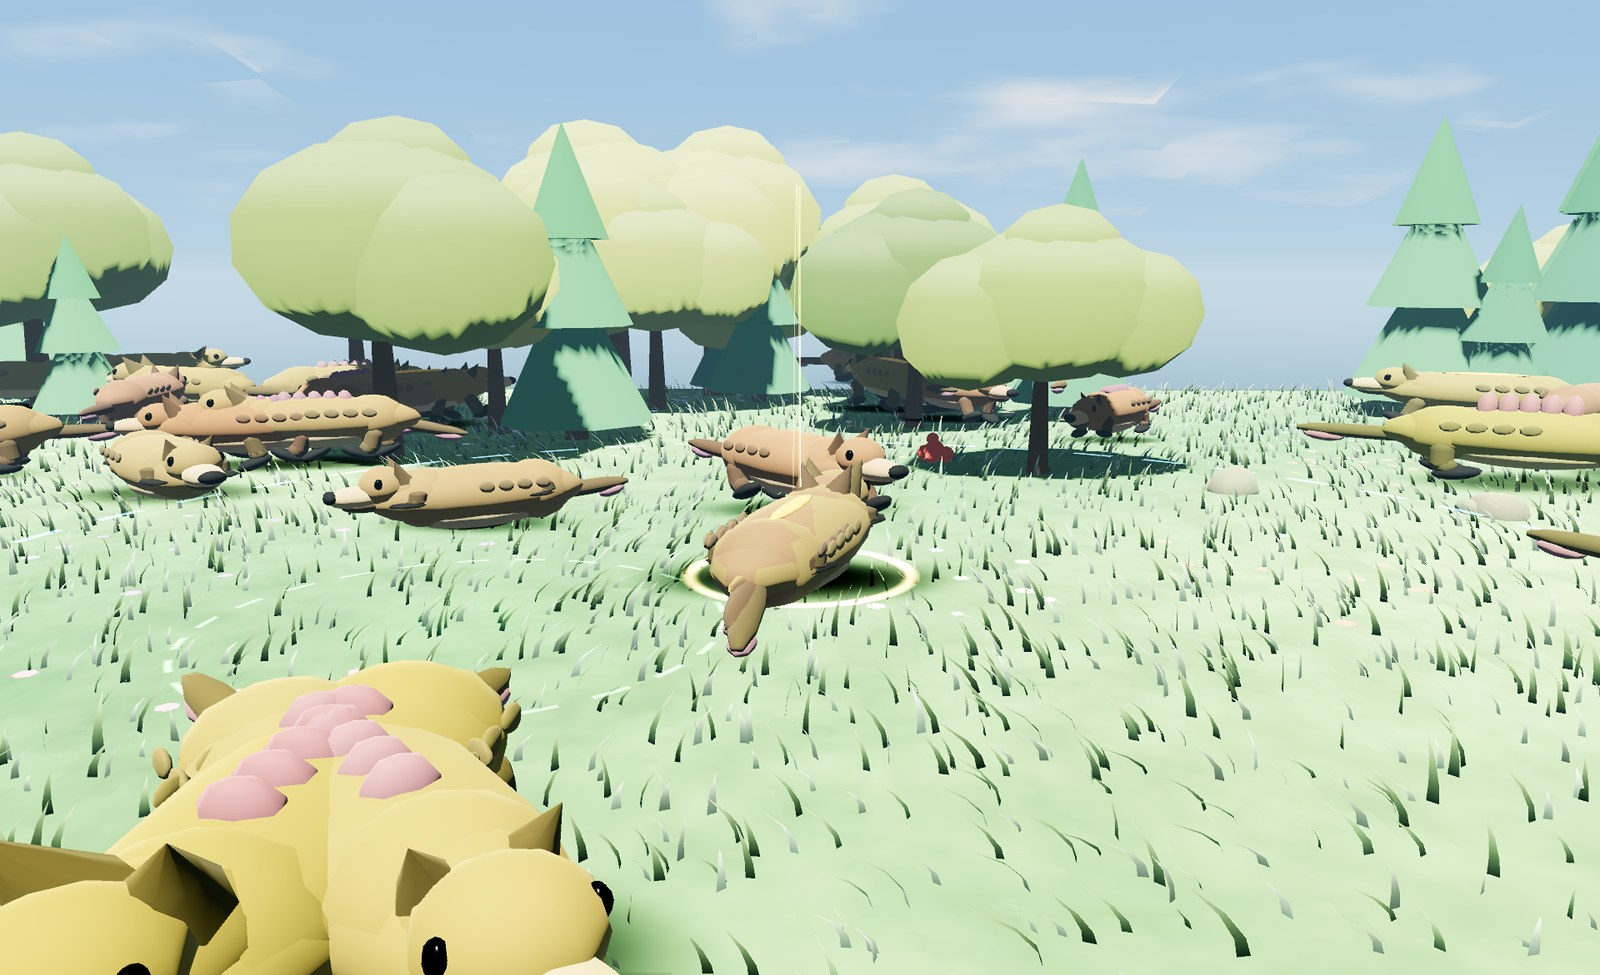
\includegraphics[width=\linewidth]{showcase-closeup.jpg}\\[-2pt]
{\small (a) Selection with kin threads}
\end{minipage}\hfill
\begin{minipage}{0.49\textwidth}\centering
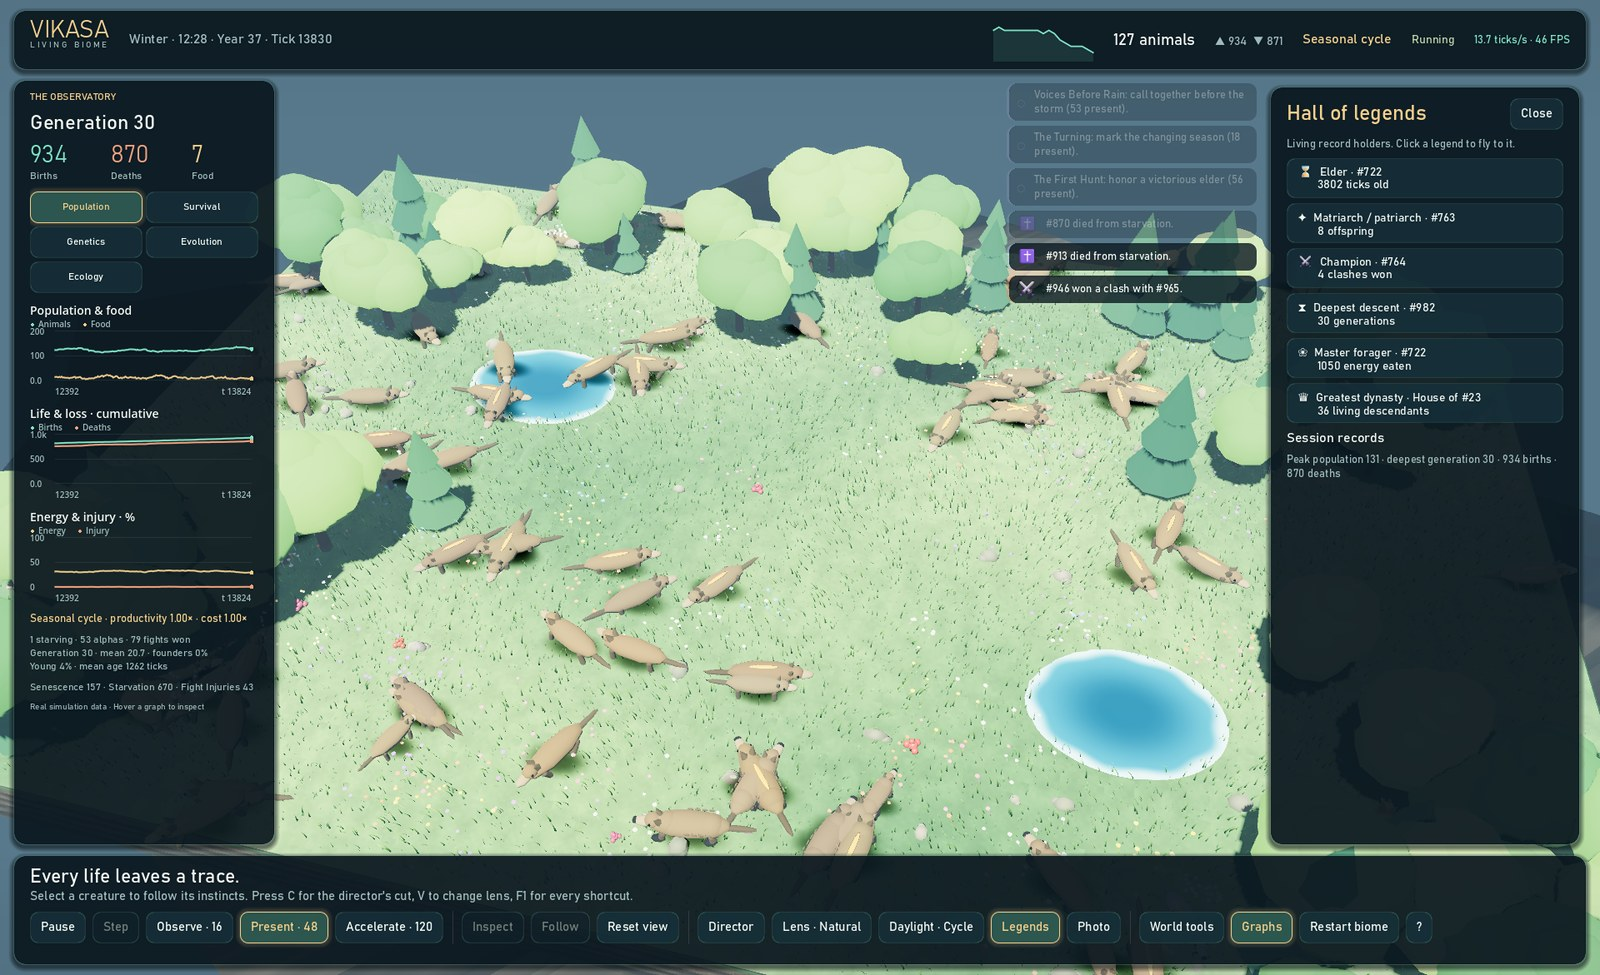
\includegraphics[width=\linewidth]{showcase-legends.jpg}\\[-2pt]
{\small (b) Hall of legends}
\end{minipage}
\caption{Inspecting individuals.}
\label{fig:closeup}
\end{figure}

\section{Species Risk Checker}
A browser application and a terminal command that, for any place and species,
return an instant estimate, an optional live simulation and a 3D replay. It is
documented fully in Chapter~\ref{ch:risk}.
\begin{lstlisting}
vikasa risk check --place hyderabad --generation-years 6 --ssp SSP5-8.5

Species Risk Checker - Hyderabad - SSP5-8.5
  Climate     mean 26.0 C, seasons +/-6.4 C (NASA POWER 1991-2020)
  Organism    generation 6 years, tolerance 9.6 C (local)
  Today       viable (peak hot season stress 0.55; breeding stops above 0.7)
  Warming     0.247 C per generation (94% of the critical rate)
  Danger line generations longer than 6.4 years fall behind under SSP5-8.5
  Survival    58% with evolution, 1% without
  VERDICT     AT RISK
\end{lstlisting}

\section{Conservation Planner}
Turns a CSV watchlist into a ranked rescue plan with breeding-failure years,
assisted gene-flow sizing, refuges and an action list; documented in
Chapter~\ref{ch:planner}.

\section{Demo mode}
\code{vikasa demo} opens a seven-chapter presenter hub (Table~\ref{tab:demo}).
Keys: $\leftarrow$/$\rightarrow$ move between chapters, Space starts the talk timer,
F toggles fullscreen and 1--7 jump directly. \code{--biome-only} opens just the 3D
autopilot.

\begin{table}[htbp]
\centering
\caption{Demo-mode chapters}
\label{tab:demo}
\begin{tabularx}{\textwidth}{clcL}
\toprule
\# & Chapter & Time & On screen \\
\midrule
1 & The question & 30 s & Headline results and the talk track \\
2 & The living biome & 90 s & One click opens the 3D biome on autopilot \\
3 & Warming in 3D & 60 s & Western Ghats seasons with rising temperature \\
4 & Species Risk Checker & 90 s & Prepared scenarios: frog in Hyderabad, six-year species, tortoise in Delhi \\
5 & The evidence & 45 s & Survival curve and all eight pre-registered criteria \\
6 & Under the hood & 45 s & Architecture and live statistics (tests, lines of code, frame rate) \\
7 & Judges' questions & --- & Prepared answers to the six most likely questions \\
\bottomrule
\end{tabularx}
\end{table}

The 3D autopilot (\code{godot/scripts/DemoPilot.gd}) runs a narrated four-minute
loop: director camera, dynasty and generation lenses, nightfall, a storm, a food
bloom and a fast-forward burst. Any key or click hands control back and restores
the user's settings. It is headless-tested by \code{godot/tests/DemoPilotSmoke.gd}.

\section{The Pygame laboratory}
\code{vikasa ui} opens the 2D laboratory with a launch configurator, presets,
organism selection, trait and lineage inspection, trails, perception overlays and
charts. Keys: Enter launches, Space pauses, 1--5 choose 1, 2, 4, 8 or 16 ticks per
rendered frame, R restarts with the same seed, C opens setup, P toggles perception,
T toggles trails, Ctrl+S saves a checkpoint, Ctrl+O loads it, E exports, and ? or
Escape opens help. Speed changes ticks per frame, never the equations.

\begin{figure}[htbp]
\centering
\begin{minipage}{0.49\textwidth}\centering
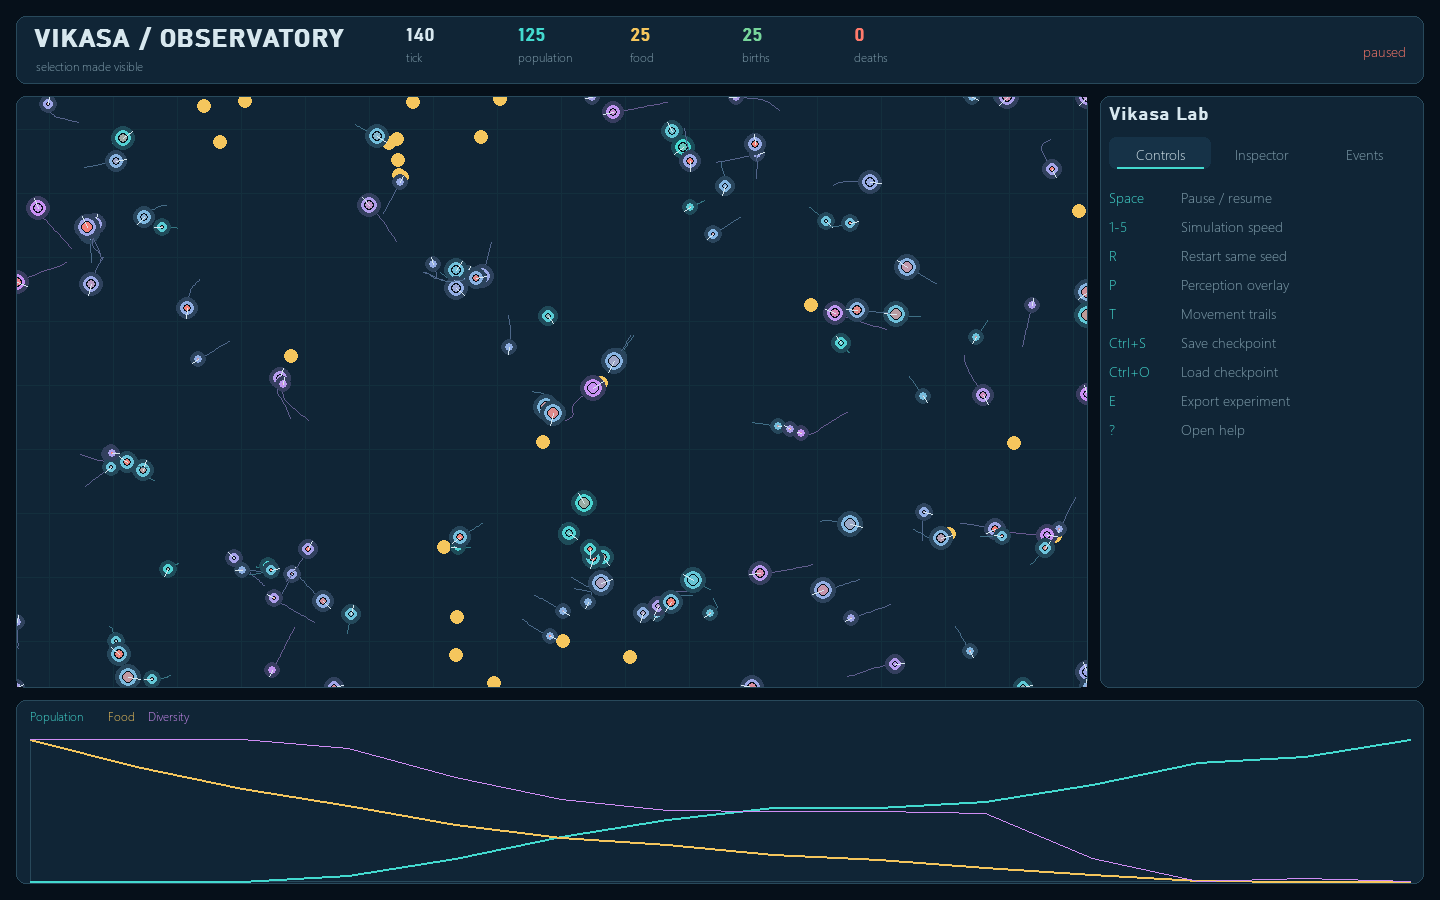
\includegraphics[width=\linewidth]{laboratory.png}\\[-2pt]
{\small (a) Laboratory view}
\end{minipage}\hfill
\begin{minipage}{0.49\textwidth}\centering
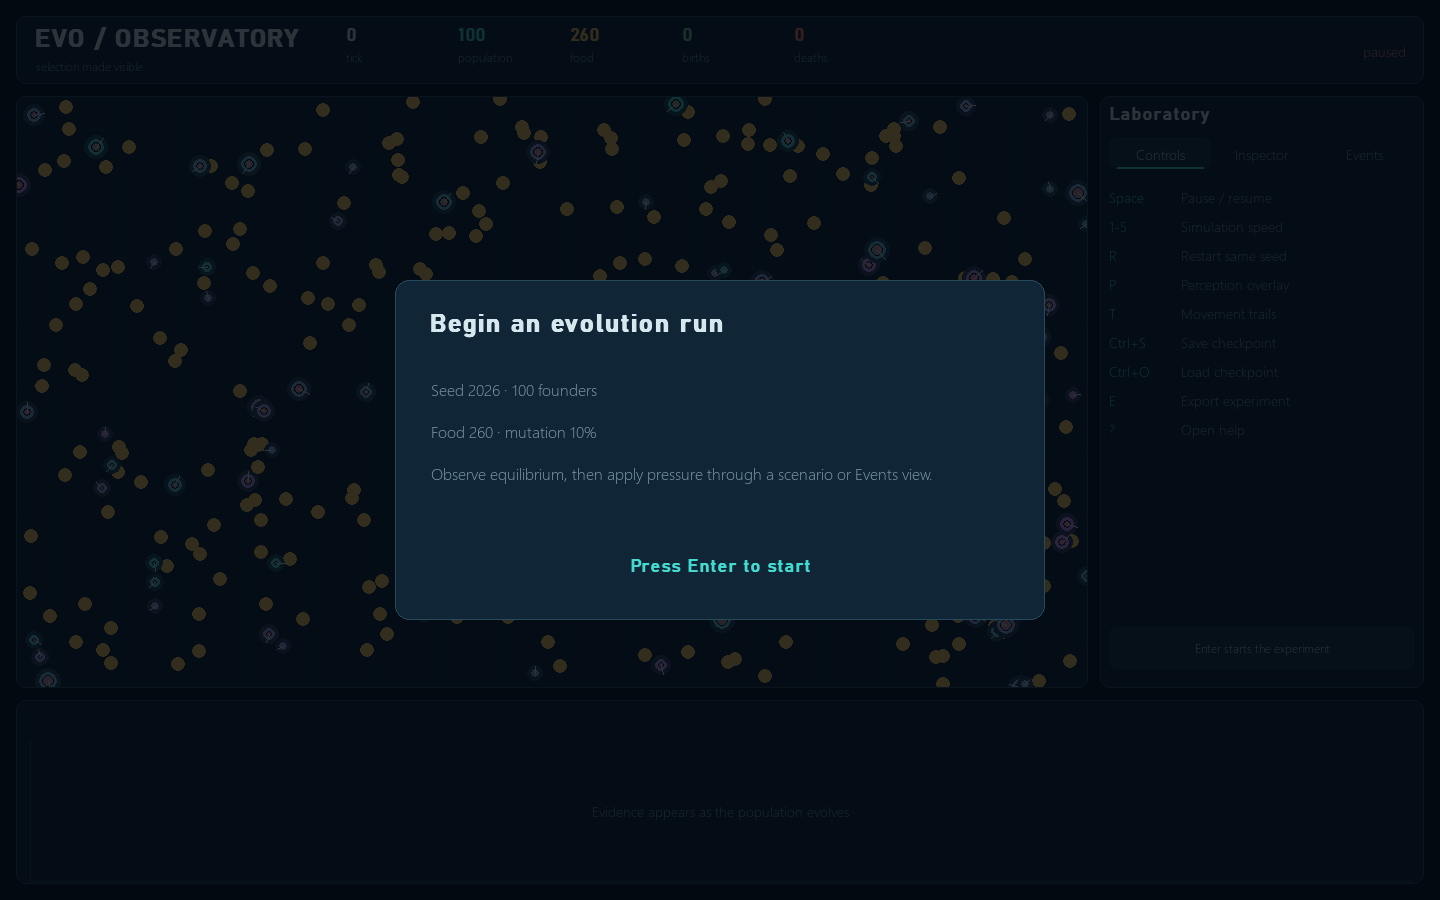
\includegraphics[width=\linewidth]{setup.png}\\[-2pt]
{\small (b) Launch configurator}
\end{minipage}
\caption{The Pygame 2D laboratory.}
\end{figure}

%===========================================================
\chapter{System Architecture}
%===========================================================

\section{Layered design}
Vikasa separates simulation outcomes from their presentation. The
\code{SimulationEngine} owns all persistent state and advances fixed,
deterministic ticks. The headless experiment runner, the
Godot Living Biome and the browser applications are \emph{clients}: they read
immutable snapshots or send explicit commands, and none of them decide creature
outcomes. Rendering can lag or disconnect without changing the simulation.

\begin{figure}[htbp]
\centering
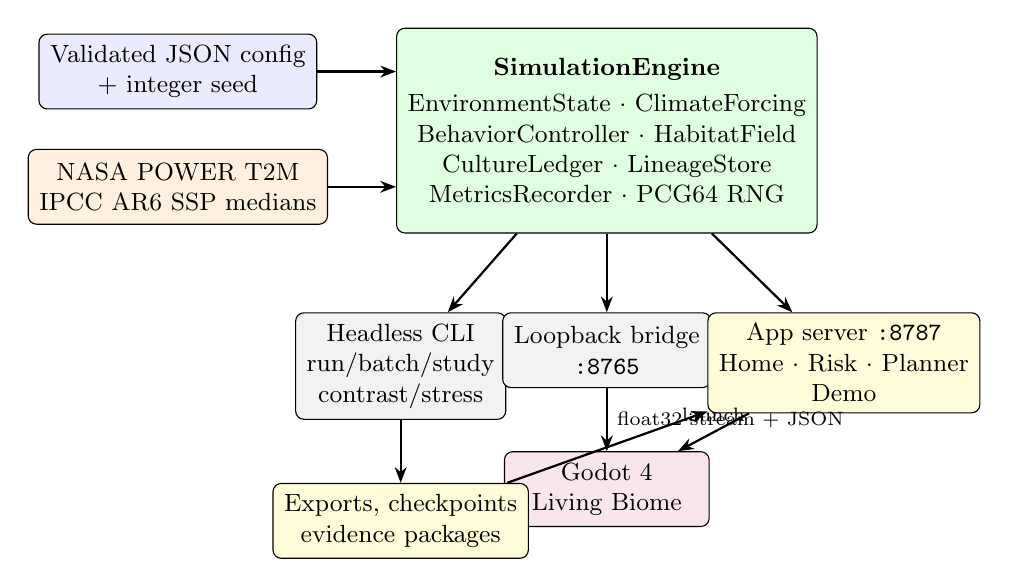
\begin{tikzpicture}[
  box/.style={draw, rounded corners=3pt, align=center, font=\small, minimum height=0.95cm, inner sep=4pt},
  arr/.style={-{Stealth[length=2mm]}, thick}]
\node[box, fill=blue!8, minimum width=3.2cm] (cfg) {Validated JSON config\\+ integer seed};
\node[box, fill=orange!12, below=0.5cm of cfg, minimum width=3.2cm] (data) {NASA POWER T2M\\IPCC AR6 SSP medians};
\node[box, fill=green!12, right=1.0cm of cfg, yshift=-0.75cm, minimum width=5.2cm, minimum height=2.6cm] (eng) {\textbf{SimulationEngine}\\[2pt]EnvironmentState $\cdot$ ClimateForcing\\BehaviorController $\cdot$ HabitatField\\CultureLedger $\cdot$ LineageStore\\MetricsRecorder $\cdot$ PCG64 RNG};
\node[box, fill=gray!10, below left=1.0cm and -1.4cm of eng, minimum width=2.6cm] (cli) {Headless CLI\\run/batch/study\\contrast/stress};
\node[box, fill=gray!10, below=1.0cm of eng, minimum width=2.4cm] (bridge) {Loopback bridge\\\code{:8765}};
\node[box, fill=yellow!15, below right=1.0cm and -1.4cm of eng, minimum width=2.8cm] (web) {App server \code{:8787}\\Home $\cdot$ Risk $\cdot$ Planner\\Demo};
\node[box, fill=purple!10, below=0.8cm of bridge, minimum width=2.6cm] (godot) {Godot 4\\Living Biome};
\node[box, fill=yellow!15, below=0.8cm of cli, minimum width=2.6cm] (out) {Exports, checkpoints\\evidence packages};
\draw[arr] (cfg) -- (eng.west |- cfg);
\draw[arr] (data) -- (eng.west |- data);
\draw[arr] (eng) -- (cli);
\draw[arr] (eng) -- (bridge);
\draw[arr] (eng) -- (web);
\draw[arr] (bridge) -- node[right,font=\scriptsize]{float32 stream + JSON} (godot);
\draw[arr] (cli) -- (out);
\draw[arr] (out) -- (web);
\draw[arr] (web) -- node[above,font=\scriptsize]{launch} (godot);
\end{tikzpicture}
\caption{Runtime architecture. Arrows show data flow; only the engine mutates the world.}
\end{figure}

\section{Module map}
\begin{longtable}{p{4.6cm}p{10.4cm}}
\caption{Python package \code{evolution\_sim}: modules and responsibilities}\\
\toprule
Module & Responsibility \\
\midrule
\endfirsthead
\toprule
Module & Responsibility \\
\midrule
\endhead
\code{config.py} & Typed, frozen, validated configuration dataclasses with defaults; strict key checking and integer/number validation; diploid architecture validation. \\
\code{model/genome.py} & Immutable six-trait \code{Genome}, optional phased haplotypes, founder sampling, clamping. \\
\code{model/genetics.py} & Arithmetic and uniform crossover, Gaussian mutation, polygenic expression and gamete formation with recombination. \\
\code{model/temperament.py} & Aggression, resilience and sociability and their inheritance. \\
\code{model/entities.py} & \code{Creature} and \code{Resource} state. \\
\code{model/lineage.py} & Parentage, birth ticks, generation depth (iterative, cycle detecting, cached). \\
\code{model/spatial.py}, \code{math2d.py} & Spatial hash for neighbour queries; 2D vector helpers and boundary handling. \\
\code{simulation/behavior.py} & Local perception contract, six drives, eight action utilities, arbitration, reason strings and targets. \\
\code{simulation/engine.py} & Tick order, movement and energy, home ranges, care, fights, food contention, reproduction, death, culture and snapshots. \\
\code{simulation/environment.py} & Seasons, scheduled events (drought, abundance, heat, cold, storm, flood, wildfire, disease, redistribute) and the optional spatial \code{HabitatField}. \\
\code{simulation/culture.py} & Cue-based traditions, contact spread and rituals. \\
\code{simulation/snapshots.py} & Immutable views for clients. \\
\code{analytics/metrics.py} & Sampled history, diversity, birth-cohort Price decomposition, invariant audits. \\
\code{analytics/trait\_space.py} & Export-time covariance, correlation, PCA and effective dimension. \\
\code{experiments/} & Scenario merging, single and batch runs, development studies, seed-blocked \code{contrast} laboratory, charts and the offline dashboard. \\
\code{io/checkpoints.py}, \code{io/export.py} & Versioned atomic checkpoints with migration; CSV/JSON/PNG exports with hash manifests. \\
\code{climate/} & Data fetching (\code{data.py}), forcing, thermal model, rescue protocol, analysis, sensitivity, surrogate, assessment, figures, report, risk checker, planner, web apps and CLI. \\
\code{bridge.py} & Loopback HTTP bridge: binary frame stream, slim explanation document, sequenced event feed, command handling, Godot launcher. \\
\code{cli.py} & The \code{vikasa} command and its sub-commands. \\
\code{shortcut.py} & Windows desktop shortcut creation. \\
\code{climate/web/} & Home screen, Risk Checker, Planner and Demo pages sharing one stylesheet (\code{vikasa.css}). \\
\bottomrule
\end{longtable}

\section{The tick}
Every tick executes the same ordered sequence (Algorithm~\ref{alg:tick-doc}).
Per-tick counters (births, deaths, combat events, recent events, fight wins) are
reset first, so each tick's outcomes are reported exactly once.

\begin{algorithm}[htbp]
\caption{\code{SimulationEngine.\_step\_once}}
\label{alg:tick-doc}
\begin{algorithmic}[1]
\State reset per-tick counters and event lists
\State \Call{environment.update}{tick} \Comment{season, climate $^{\circ}$C, events}
\If{spatial habitat enabled} \State \Call{habitat.step}{environment} \EndIf
\State erode existing food by $\min(0.4,\text{resource\_decay})$; drop patches $<1$ energy
\State regenerate food (spawn accumulator, seasonal and event multipliers)
\State build resource index; perceive, decide (staggered), move and pay energy
\If{$\text{tick} \bmod 4 = 0$} \State resolve contests \EndIf
\State resolve feeding contention (squared distance, then stable ID)
\State resolve paired reproduction (Price observer records the cohort)
\State resolve deaths (starvation, injury, senescence, age ceiling, exposure)
\State $\text{tick}\gets\text{tick}+1$
\State culture update; satisfaction update
\If{$\text{tick} \bmod \text{sample\_interval} = 0$} record metrics \EndIf
\end{algorithmic}
\end{algorithm}

\subsection{Adaptive cognition schedule}
Behaviour decisions are the most expensive per-animal step. When the population
exceeds \code{ADAPTIVE\_DECISION\_POPULATION} $=40$, each animal re-decides only
when $(\text{tick}+\text{id}) \bmod 6 = 0$ (\code{ADAPTIVE\_DECISION\_INTERVAL}
$=6$); between decisions it continues its current action. Movement, hunger,
consumption, births and deaths still advance every tick. Contest opportunities are
evaluated every four ticks (\code{COMBAT\_EVALUATION\_INTERVAL} $=4$). These
schedules are deterministic and apply identically to GUI and headless runs.

\section{Determinism contract}
A run is reproducible when the configuration, seed, scheduled events, tick count,
software version and numerical platform are equal. The engine guarantees this by:
\begin{itemize}[leftmargin=*]
\item one NumPy PCG64 generator for every stochastic outcome;
\item iteration over creatures and resources in sorted stable-ID order;
\item explicit tie-breaking (squared distance, then ID) for contested food;
\item a fractional food-spawn accumulator stored in checkpoints;
\item observers (Price, PCA, metrics, bootstrap) that never consume engine RNG;
\item wall-clock rendering that never feeds back into outcomes. Only explicitly
issued world-tool commands change the world, and they are logged as interventions.
\end{itemize}

\section{Concurrency model}
The bridge runs the engine in a background thread under a lock. Commands are
serialised under the same lock and publish their result immediately. Readers
receive the last published frame and document without waiting for the simulation
lock, which keeps presentation responsive at high requested tick rates. If the
host cannot achieve the requested rate, excess catch-up work is dropped instead of
accumulating, and the HUD reports the measured rate alongside the requested one.

%===========================================================
\chapter{Configuration Reference}
%===========================================================

Configurations are JSON files parsed into frozen dataclasses. Unknown keys,
missing required keys, booleans in place of numbers and fractional values in
integer fields are rejected with a \code{ConfigError} that names the exact path.

\section{Root keys}
\begin{table}[htbp]
\centering
\caption{Root configuration keys}
\begin{tabularx}{\textwidth}{llL}
\toprule
Key & Type & Meaning \\
\midrule
\code{world} & object & \code{width}, \code{height} (units) and \code{boundary} (\code{collision} or \code{wrap}). \\
\code{genome} & object & Trait bounds, mutation probability and sigma, crossover type, optional diploid architecture. \\
\code{energy} & object & \code{initial}, \code{basal\_cost}, \code{movement\_cost}, \code{maximum}. \\
\code{reproduction} & object & \code{minimum\_age}, \code{cooldown}, \code{mate\_radius}, \code{offspring\_energy}, \code{population\_cap}. \\
\code{resources} & object & \code{initial\_count}, \code{spawn\_rate}, \code{maximum\_count}, \code{energy\_value}. \\
\code{metrics} & object & \code{sample\_interval}, \code{diversity\_sample}. \\
\code{initial\_population} & int & Number of founders. \\
\code{maximum\_age} & int & Hard age ceiling in ticks. \\
\code{wander\_change\_probability} & float & Per-tick chance to change wander heading. \\
\code{behavior} & object & Optional; see Table~\ref{tab:behavior}. \\
\code{demography} & object & Optional; \code{fixed} or \code{gompertz} mortality. \\
\code{ecology} & object & Optional spatial plant/water field. \\
\code{climate} & object & Optional observed-temperature forcing and thermal tolerance. \\
\bottomrule
\end{tabularx}
\end{table}

\section{Showcase values}
\begin{table}[htbp]
\centering
\caption{\code{config/showcase.json} (default 3D world)}
\begin{tabularx}{\textwidth}{lLl}
\toprule
Section & Parameter & Value \\
\midrule
world & width $\times$ height, boundary & $720\times480$, collision \\
genome & size / speed & [2.5, 8.0] / [0.5, 4.0] \\
 & perception / metabolism & [25, 150] / [0.65, 1.5] \\
 & reproduction threshold / fertility & [70, 150] / [0.15, 0.55] \\
 & mutation probability, sigma, crossover & 0.1, 0.075, arithmetic \\
energy & initial, basal, movement, maximum & 125, 0.09, 0.026, 230 \\
reproduction & min. age, cooldown, mate radius & 90, 100, 90 \\
 & offspring energy, population cap & 60, 180 \\
resources & initial, spawn rate, max, energy & 180, 0.9, 400, 30 \\
metrics & sample interval, diversity sample & 8, 48 \\
root & founders, maximum age, wander & 64, 12000, 0.03 \\
demography & mode, $\mu_0$, $a_0$, $b$ & gompertz, 0.00002, 1800, 0.002 \\
\bottomrule
\end{tabularx}
\end{table}

\section{Behaviour, demography, ecology and climate sections}
\begin{table}[htbp]
\centering
\caption{\code{behavior} defaults and validation}
\label{tab:behavior}
\begin{tabularx}{\textwidth}{llL}
\toprule
Key & Default & Meaning and range \\
\midrule
\code{hysteresis\_margin} & 0.08 & Keep the current action if within this utility of the best; $[0,1]$. \\
\code{softmax\_temperature} & 0.08 & Near-tie softmax temperature $\tau$; $[0.001,1]$. \\
\code{dependent\_age\_ticks} & 240 & Age below which offspring are dependents. \\
\code{care\_radius} & 24 & Maximum parent--offspring distance for care. \\
\code{care\_energy\_rate} & 0.25 & Energy transferred per care tick (parent reserve protected). \\
\code{danger\_preempt\_threshold} & 0.75 & Danger at/above this forces flight; $[0,1]$. \\
\code{territory\_migration\_margin} & 0.15 & Outside-food advantage needed to shift a home range. \\
\bottomrule
\end{tabularx}
\end{table}

\begin{table}[htbp]
\centering
\caption{\code{demography}, \code{ecology} and \code{climate} defaults}
\begin{tabularx}{\textwidth}{llL}
\toprule
Key & Default & Meaning \\
\midrule
\code{demography.mode} & fixed & \code{fixed} age ceiling or \code{gompertz} hazard. \\
\code{background\_hazard} & 0.00002 & Baseline hazard $\mu_0$ per tick. \\
\code{senescence\_age}, \code{\_rate} & 1800, 0.002 & Onset $a_0$ and exponential rate $b$. \\
\midrule
\code{ecology.enabled} & false & Enables the plant/water field. \\
\code{columns}, \code{rows} & 24, 16 & Grid size, each $\le 64$. \\
\code{capacity}, \code{initial\_fraction} & 100, 0.65 & Plant capacity $K$ per cell, initial fill. \\
\code{growth\_rate} & 0.006 & Logistic rate $r$. \\
\code{rainfall\_rate}, \code{evaporation\_rate} & 0.004, 0.002 & Bucket inflow and loss. \\
\code{water\_diffusion}, \code{biomass\_diffusion} & 0.06, 0.008 & Transport coefficients $d\le 1/4$. \\
\code{water\_half\_saturation} & 0.25 & Moisture response $h$. \\
\code{transpiration\_rate} & 0.03 & Water used per unit growth. \\
\midrule
\code{climate.enabled} & false & Enables observed forcing. \\
\code{ticks\_per\_year} & 384 & Climate year length in ticks ($\ge4$). \\
\code{monthly\_c} & 12 $\times$ 25.0 & Monthly climatology, each in $[-60,60]$\,$^{\circ}$C. \\
\code{anomaly\_c} & [] & Warming knots $[\text{year},\Delta]$. \\
\code{tolerance\_breadth\_c} & 4.0 & Cold-side breadth $\omega$. \\
\code{warm\_side\_ratio} & 0.6 & Warm-side width multiplier. \\
\code{stress\_metabolic\_gain} & 1.5 & Basal cost $\times(1+1.5\varsigma)$. \\
\code{stress\_injury\_rate} & 0.02 & Injury per tick above $\varsigma=0.3$. \\
\code{fertility\_stress\_limit} & 0.7 & No breeding above this stress. \\
\code{inheritance} & heritable & \code{heritable} or \code{none} (control). \\
\code{founder\_mean\_c}, \code{founder\_sd\_c} & auto, 1.0 & Founder optimum distribution. \\
\code{segregation\_sd\_c}, \code{mutation\_sd\_c} & 0.4, 0.1 & Offspring noise terms. \\
\bottomrule
\end{tabularx}
\end{table}

The ecology validator enforces the explicit-diffusion stability limit: both
diffusion coefficients must not exceed $1/4$. The diploid architecture validator
requires six effect rows of equal length (2--64 loci), dominance in $[-1,1]$,
recombination in $[0,0.5]$ for each of the $L-1$ intervals, founder frequencies in
$[0,1]$ and an allele mutation probability in $[0,1]$.

\section{Bundled configurations and scenarios}
\begin{table}[htbp]
\centering
\caption{Configuration and scenario files}
\begin{tabularx}{\textwidth}{lL}
\toprule
File & Purpose \\
\midrule
\code{config/default.json} & Baseline world used by the headless scenarios. \\
\code{config/showcase.json} & Sustained 3D showcase (64 founders, cap 180, Gompertz). \\
\code{config/extinction-control.json} & Preserved extinction-prone earlier showcase for comparison. \\
\code{config/spatial-biome.json} & Research profile with the plant/water field. \\
\code{config/diploid-biome.json} & Opt-in chromosome preview (unreleased). \\
\code{config/climate-rescue.json} & $480\times320$ rescue world used by the climate sweep. \\
\code{config/climate-demo.json} & Warming demo for the 3D client with live $^{\circ}$C readout. \\
\code{experiments/*.json} & Scenarios: baseline, scarcity, mutation\_high/low, environmental\_shift, diploid-biome, weather-contrast(-preview). \\
\bottomrule
\end{tabularx}
\end{table}

A scenario file names a base configuration and deep-merges overrides into it, and
may schedule environmental events, a default seed and a horizon. The bundled
\code{experiments/scarcity.json}:
\begin{lstlisting}
{ "name": "scarcity",
  "description": "A sustained drought exposes energy and sensing trade-offs.",
  "config": "../config/default.json",
  "seed": 2202, "ticks": 7000, "overrides": {},
  "events": [ {"kind": "drought", "start_tick": 1800, "duration": 4200,
               "intensity": 0.22, "label": "Sustained drought"} ] }
\end{lstlisting}
Contrast protocols (Chapter~\ref{ch:experiments}) extend this with a control arm,
seed list, sampling interval, bootstrap seed and sample count, and a list of
\code{arms}, each with its own overrides and events. The weather preview, for
example, declares seeds 2026, 7 and 41, 800 ticks, sampling every 20 ticks,
bootstrap seed 271828 and 4{,}096 bootstrap samples on the spatial-biome base.

%===========================================================
\chapter{Genome and Inheritance}
%===========================================================

\section{The six-gene body genome}
Every animal carries an immutable \code{Genome}: an ordered vector of six bounded
quantitative traits,
\[
\mathbf{g}=(\text{size},\ \text{speed},\ \text{perception},\ \text{metabolism},\ \text{reproduction\_threshold},\ \text{fertility}),
\qquad g_i\in[L_i,H_i].
\]
Each value must be finite and inside its configured bounds; a genome built from a
mapping must contain exactly these six keys.

\begin{table}[htbp]
\centering
\caption{Body genes and their effects}
\begin{tabularx}{\textwidth}{lL}
\toprule
Gene & Effect in the model \\
\midrule
size & Raises basal and movement cost; strengthens contests and defence. \\
speed & Faster travel and access; raises movement cost and travel utility cost. \\
perception & Radius for sensing food, mates, threats; does not guarantee capture. \\
metabolism & Divides basal cost: higher metabolism means \emph{better} basal efficiency in this code base. \\
reproduction\_threshold & Energy an animal must hold to be eligible to mate. \\
fertility & Shortens mating cooldown: $\max(1,\mathrm{round}(c(1-0.5f)))$. \\
\bottomrule
\end{tabularx}
\end{table}

\subsection{Founders}
Each founder gene is drawn independently and uniformly, $g_i\sim U(L_i,H_i)$.

\subsection{Crossover}
Two operators are configurable. \emph{Arithmetic} crossover draws an independent
$\alpha_i\sim U(0,1)$ per gene and sets
\[
c_i=\alpha_i a_i+(1-\alpha_i)b_i,
\]
so offspring lie between their parents. \emph{Uniform} crossover takes each gene
from one parent with probability $1/2$.

\subsection{Mutation}
Independently per gene, a Bernoulli trial with probability $p_m$ gates a Gaussian
perturbation scaled to the gene's span, then the value is clamped:
\[
g'_i=\mathrm{clamp}_{[L_i,H_i]}\big(c_i+\varepsilon_i\big),\qquad
\varepsilon_i\sim\mathcal{N}\big(0,\ \sigma(H_i-L_i)\big)\ \text{with prob. } p_m.
\]
The showcase uses $p_m=0.1$ and $\sigma=0.075$, so a mutated gene typically moves
by 7.5\% of its range.

\section{Temperament}
Aggression, resilience and sociability are inherited separately from the body
genome, each in $[0,1]$. Offspring values combine the parental values with seeded
Gaussian variation and are clipped to $[0,1]$. Aggression raises contest risk and
strength; resilience reduces exposure injury and strengthens defence; sociability
raises mating and care drives and influences tradition founding.

\section{The opt-in diploid architecture}
\code{config/diploid-biome.json} enables an explicit chromosome model. It is an
unreleased research preview; the default showcase does not use it.

Each animal carries two phased binary haplotypes $h^{(1)},h^{(2)}\in\{0,1\}^L$
with $2\le L\le64$ loci on one linked chromosome. Expression proceeds in three
steps. First, a dominance-adjusted dosage per locus,
\[
\delta_\ell=\frac{h^{(1)}_\ell+h^{(2)}_\ell}{2}+d_\ell\,\frac{|h^{(1)}_\ell-h^{(2)}_\ell|}{2},
\qquad d_\ell\in[-1,1].
\]
Second, each trait's effect row $\mathbf{e}_j$ is normalised to unit absolute mass
and applied around the midpoint,
\[
n_j=\mathrm{clip}\Big(0.5+\sum_\ell \frac{e_{j\ell}}{\sum_k|e_{jk}|}\,(\delta_\ell-0.5)\Big).
\]
Third, the trait is mapped into its bounds: $g_j=L_j+n_j(H_j-L_j)$.

Meiosis starts on a random homologue and switches homologue in interval $\ell$
with probability $r_\ell\in[0,0.5]$, producing one recombinant gamete per parent.
Founders draw each allele as 1 with the configured founder frequency. Figure
\ref{fig:diploid} shows the preview's allele frequencies, heterozygosity, linkage
association and individual dosages.

\begin{figure}[htbp]
\centering
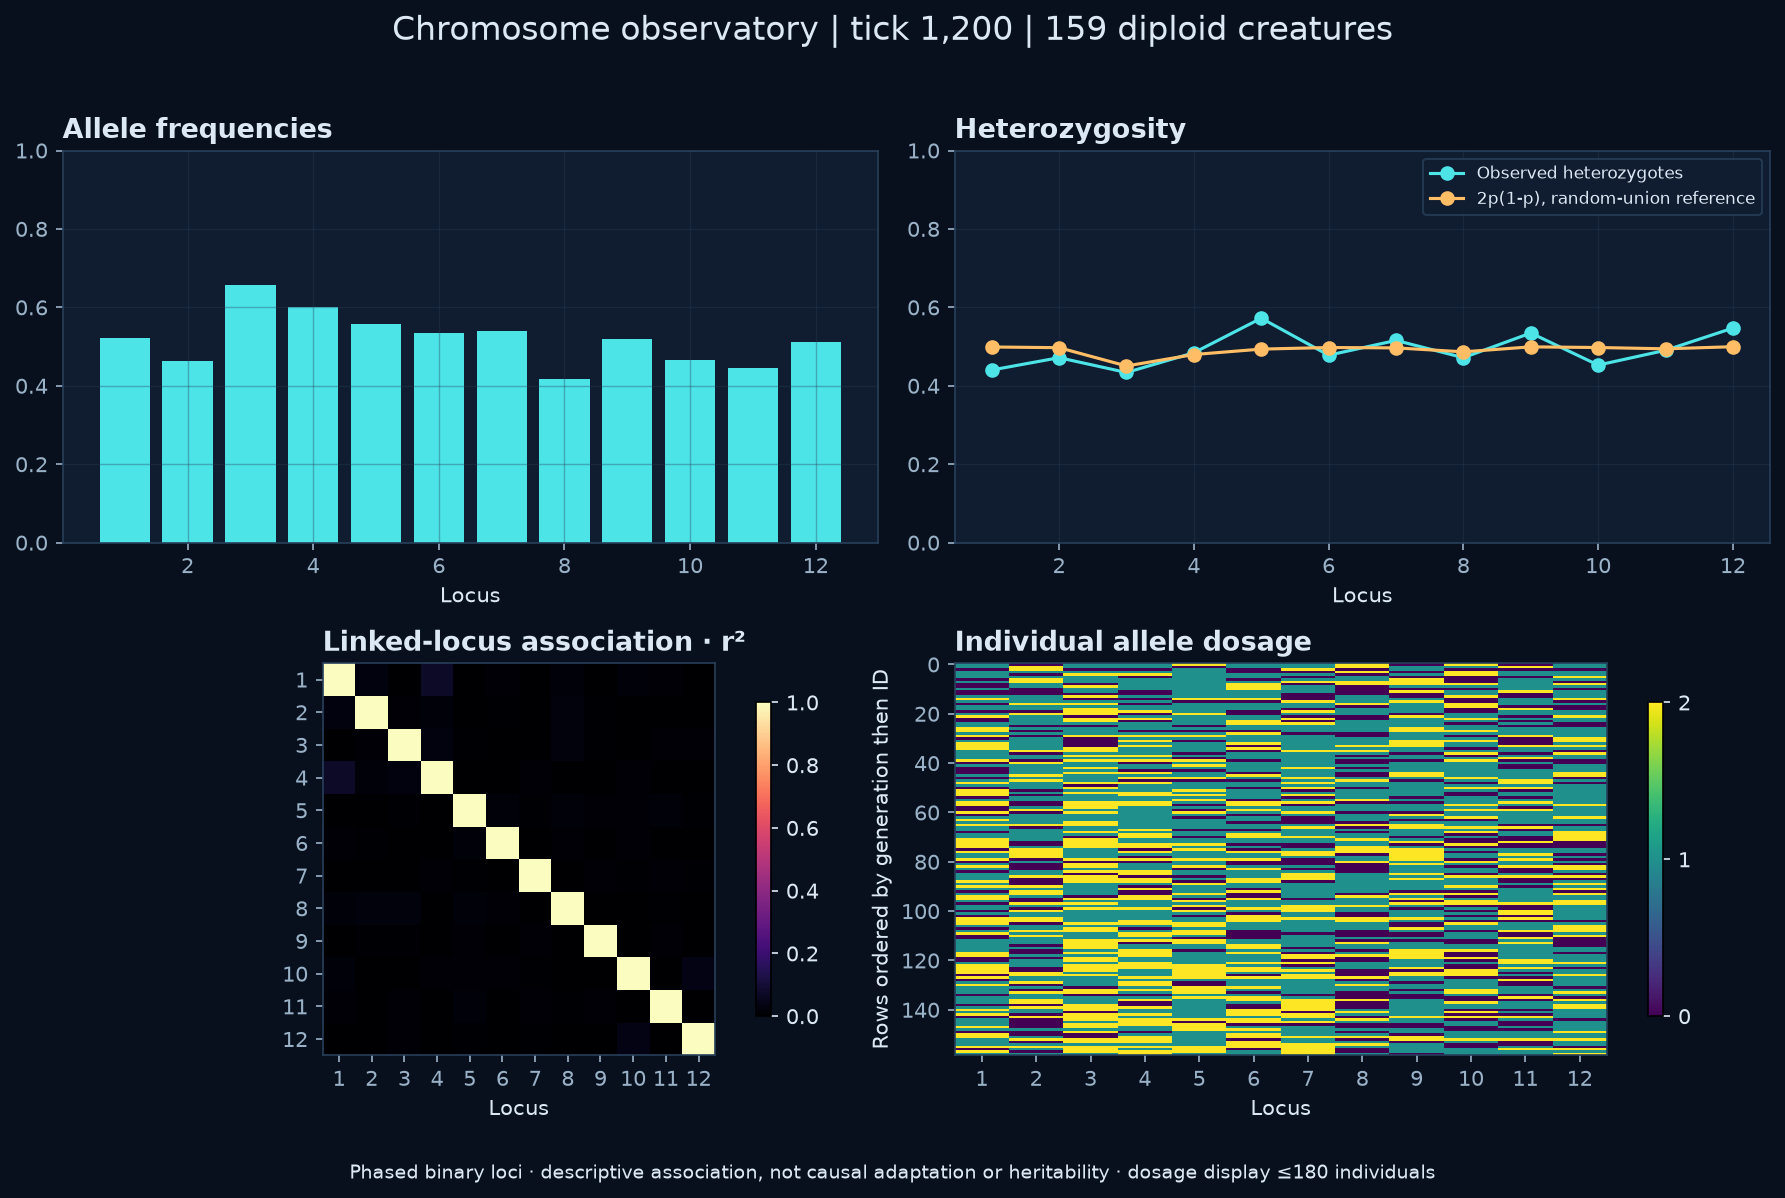
\includegraphics[width=0.92\textwidth]{chromosomes.png}
\caption{Diploid preview (seed 2026, tick 1{,}200): allele frequencies,
heterozygosity against the $2p(1-p)$ reference, linked-locus $r^2$ and individual
dosages. One development run; not long-horizon validation.}
\label{fig:diploid}
\end{figure}

\section{Heritable thermal optimum}
When climate forcing is enabled, each animal also carries a thermal optimum
$\theta$ in $^{\circ}$C, clamped to $[-20,60]$. Founders draw
$\theta\sim\mathcal{N}(\mu_f,\sigma_f)$ where $\mu_f$ defaults to the local annual
mean plus the starting anomaly and $\sigma_f=1\,^{\circ}$C. Offspring follow the
infinitesimal model:
\[
\theta_{\text{child}}=\frac{\theta_1+\theta_2}{2}+\mathcal{N}(0,\sigma_s)+\mathcal{N}(0,\sigma_\mu),
\qquad \sigma_s=0.4,\ \sigma_\mu=0.1.
\]
With \code{inheritance = "none"} the offspring optimum is instead drawn afresh from
the founder distribution: the control arm has the same spread but zero heritability.

%===========================================================
\chapter{Behaviour: Drives, Utilities and Arbitration}
%===========================================================

\section{Perception}
Each decision receives a tick-local perception: food patches, eligible mates,
threats and dependent offspring within the animal's perception radius, plus global
hazard and terrain pressures and the animal's own home-range displacement. The
perception is a contract: behaviour never reads the world directly.

\section{The six drives}
Drives are normalised pressures in $[0,1]$, stored and displayed in a fixed order.
With $E$ the energy, $E_{\max}$ the maximum and $I$ the injury:
\begin{align*}
\text{deficit}&=\mathrm{clip}(1-E/E_{\max})\\
\text{survival}&=\mathrm{clip}\big(0.65(1-E/E_{\max})+0.35I\big)\\
\text{hunger}&=\max(\text{stored\_hunger},\ \text{deficit})\\
\text{foraging}&=\mathrm{clip}\big(\text{hunger}\,(0.5+0.5\,\text{best\_food\_reward})\big)\quad\text{if food is sensed, else }0\\
\text{danger}&=\max(\text{local\_hazard},\ \text{best\_threat\_pressure})
\end{align*}
Food reward is
$\mathrm{clip}\big(\text{food\_energy}/\max(1,0.15E_{\max})\big)\cdot\mathrm{clip}(1-\text{distance}/\text{perception})$.
Threat pressure combines proximity, the threat's aggression, relative size and the
receiver's injury, each bounded to $[0,1]$.

\textbf{Mating} is zero unless the animal and at least one perceived mate are
eligible, survival is below 0.55 and injury below 0.65; otherwise
\[
\text{mating}=\mathrm{clip}\big((0.5+0.5E/E_{\max})\cdot\text{proximity}\cdot(0.7+0.3\,\text{sociability})\big).
\]
\textbf{Offspring care} is the maximum over nearby dependents $j$ of
\begin{multline*}
\mathrm{clip}\big(0.35(1-\text{age}_j/\text{dependent\_age})+0.45\,\mathrm{clip}(1-E_j/E_{\max})\\
+0.20\max(I_j,\text{danger})\big)\cdot(0.6+0.4\,\text{sociability}).
\end{multline*}
\textbf{Territory}, with $d$ the distance from the home centre and $r$ the home radius:
\[
\text{territory}=\mathrm{clip}(0.35+0.65\,d/r)\,(1-0.75\,\text{hunger})\,(1-0.5\,\text{danger}).
\]

\begin{figure}[htbp]
\centering
\begin{minipage}{0.49\textwidth}\centering
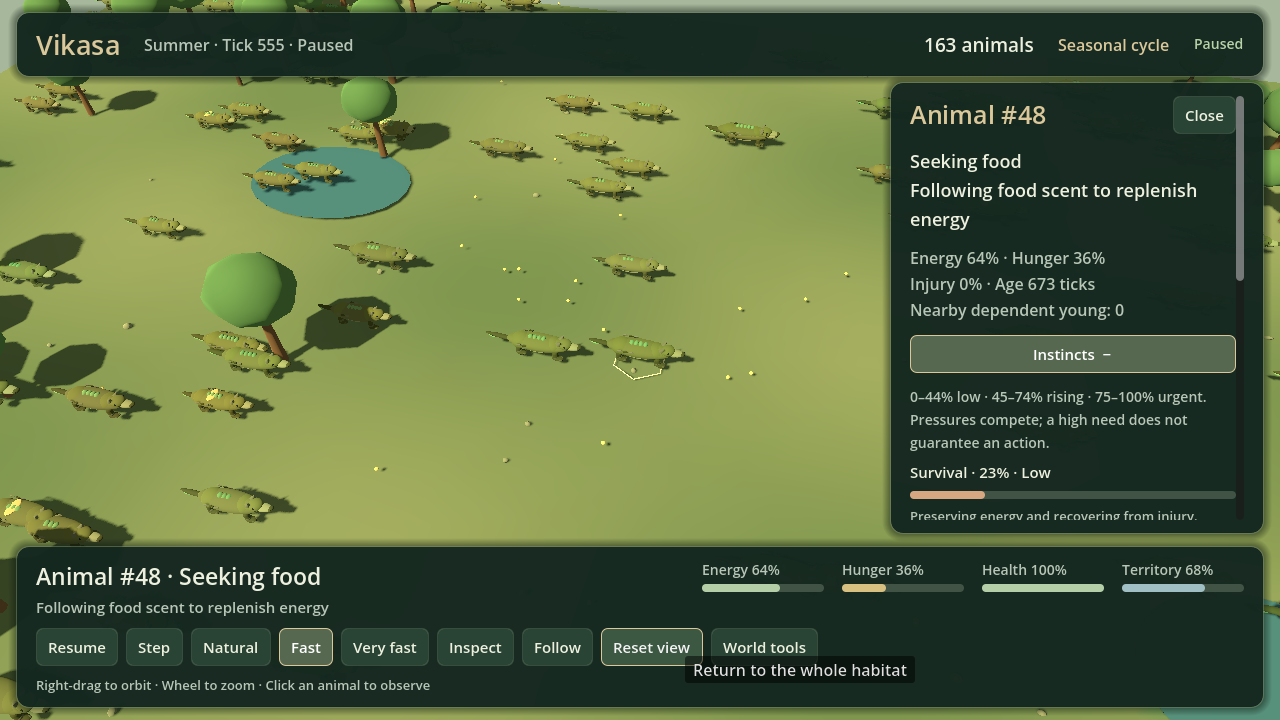
\includegraphics[width=\linewidth]{wildlife-instincts.png}\\[-2pt]
{\small (a) Instincts panel}
\end{minipage}\hfill
\begin{minipage}{0.49\textwidth}\centering
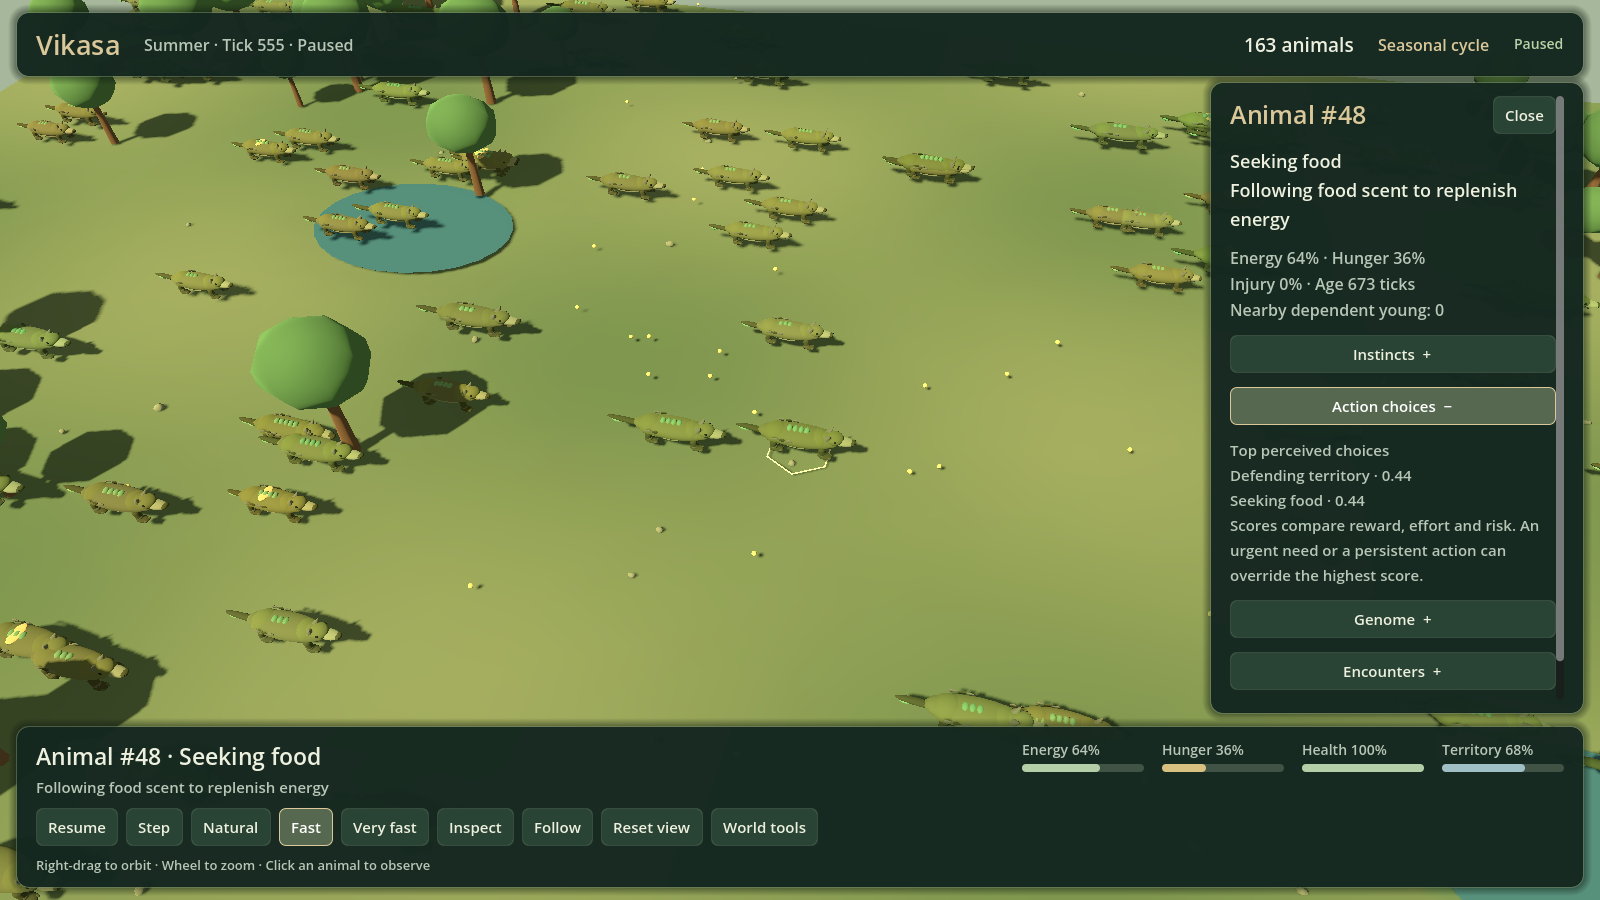
\includegraphics[width=\linewidth]{wildlife-action-choices.png}\\[-2pt]
{\small (b) Action choices panel}
\end{minipage}
\caption{The inspector exposes the six drives and the leading action utilities.}
\end{figure}

\section{Action utilities}
Eight actions compete. For action $a$ with affinity vector $\mathbf{A}_a$ over the
six drives $\mathbf{D}$:
\[
U_a=\mathrm{clip}\Big(\textstyle\sum_k A_{a,k}D_k+R_a-T_a-X_a-K_a\Big)
\]
where $R_a$ is an action-specific reward (local food value, relief from survival
pressure, dependent need, danger or territory context) and the costs are
\begin{align*}
T_a&=0.12\,\mathrm{clip}(\text{distance}/\text{perception})\,\frac{\text{speed}/4}{\text{metabolism}}+0.08\,\text{terrain\_cost}\quad(\text{not for rest})\\
X_a&=\begin{cases}0.05\,\text{danger}&\text{rest}\\0&\text{flee}\\0.25\,\text{danger}&\text{otherwise}\end{cases}\qquad
K_a=\begin{cases}0.15\,\text{danger}&\text{seek mate}\\0.30\,\text{danger}/\text{relative strength}&\text{challenge}\\0&\text{otherwise.}\end{cases}
\end{align*}

\begin{table}[htbp]
\centering
\caption{Action affinities over (survival, foraging, mating, care, danger, territory)}
\begin{tabular}{lcccccc}
\toprule
Action & Surv. & Forage & Mate & Care & Danger & Terr. \\
\midrule
explore & 0.10 & 0.15 & 0 & 0 & 0 & 0 \\
forage & 0.35 & 0.65 & 0 & 0 & 0 & 0 \\
rest & 0.55 & 0 & 0 & 0 & 0 & 0 \\
seek mate & 0 & 0 & 0.65 & 0 & 0 & 0 \\
care & 0 & 0 & 0 & 0.75 & 0 & 0 \\
flee & 0.15 & 0 & 0 & 0 & 0.85 & 0 \\
patrol & 0 & 0 & 0 & 0 & 0 & 0.65 \\
challenge & 0 & 0 & 0 & 0 & 0 & 0.45 \\
\bottomrule
\end{tabular}
\end{table}

\section{Arbitration}
\begin{enumerate}[leftmargin=*]
\item Actions without a valid opportunity (no food, no mate, no dependent, no
rival) are \emph{excluded}, not given a fabricated competing score.
\item Danger at or above the preemption threshold (0.75) forces \emph{flee}.
\item Survival pressure at or above 0.65 forces \emph{forage} when food is sensed,
otherwise \emph{explore}. Injury at or above 0.65 forces \emph{rest}.
\item Otherwise the current action is retained if its utility is within the
hysteresis margin (0.08) of the best candidate, which prevents jitter.
\item Remaining near-ties within the softmax temperature $\tau$ are resolved with
seeded probabilities $P(a)=\exp((U_a-U_{\max})/\tau)/\sum_j\exp((U_j-U_{\max})/\tau)$.
\end{enumerate}
High need therefore does not guarantee the matching action: opportunity, travel,
danger, conflict, preemption and persistence all matter. Each decision records the
action, its target, the start tick, the full utility breakdown and a
human-readable reason (at most 240 characters). The base reasons are: explore
``Searching nearby for better habitat'', forage ``Following food scent to replenish
energy'', rest ``Resting to conserve energy and recover'', seek mate ``Approaching an
eligible mate'', care ``Staying near hungry or vulnerable young'', flee ``Moving away
from danger'', patrol ``Returning toward the home range'' and challenge ``Defending
the home range under local competition''.

\section{Home range, patrol, care and migration}
Each animal has a home-range centre and a radius (sampled deterministically per
creature). \emph{Patrol} chooses a persistent waypoint near the range edge.
\emph{Care} lets a parent feed living offspring younger than the dependent age and
within the care radius, transferring a limited amount of energy while protecting
the parent's own reserve. \emph{Migration} is a small local-resource response: if
an animal remains outside its range while foraging, and the perceived outside food
reward exceeds the inside reward by the migration margin (0.15) for 24 consecutive
qualifying ticks, its centre shifts 0.5\% toward its position.

%===========================================================
\chapter{Energy, Survival and Mortality}
%===========================================================

\section{Energy budget}
Basal expenditure per tick is
\[
C_b=c_b\,\frac{1+\text{size}/8}{\text{metabolism}}\;
\mu_{\text{event}}\,\mu_{\text{season}}\,\mu_{\text{injury}}\,\mu_{\text{health}}\,(1+1.5\,\varsigma),
\]
where the last factor applies only with climate forcing. Movement expenditure is
\[
C_m=c_m\cdot\text{distance}\cdot(0.5+\text{size}/8)\,(0.5+\text{speed}/4)\cdot\mu_{\text{weather}}.
\]
Energy is clamped at $E_{\max}$ after food gain and costs. Food is consumed once
and supplies the patch's remaining energy; competing animals resolve access by
squared distance, then stable ID.

\section{Starvation}
Hunger is $\mathrm{clip}(1-E/E_{\max})$. At non-positive energy a starvation
counter increases by one per tick; when energy is positive it decreases by one, to
a floor of zero. Death occurs at 12 accumulated starvation ticks. Starvation is
therefore delayed and reversible, not a single-tick deletion.

\section{Exposure injury}
Under health pressure $H$ (from weather events, Chapter~\ref{ch:env}) injury rises
by
\[
\Delta I=0.018\,H\,(1-0.75\,\text{resilience})\,(1+0.6\,\text{hunger}),\qquad I'=\min(1,I+\Delta I).
\]
Lethal injury is $I\ge0.98$. With active health pressure it is attributed to
environmental exposure, otherwise to fight injuries; with mixed causes the
attribution is approximate. Calm-weather recovery is unchanged.

\section{Thermal stress}
With climate forcing (Chapter~\ref{ch:climate}) thermal stress $\varsigma$ is
computed in the energy step before the basal cost. It multiplies the basal cost by
$1+1.5\varsigma$, adds injury $0.02(\varsigma-0.3)/0.7$ per tick when
$\varsigma>0.3$, and blocks reproduction while $\varsigma>0.7$.

\section{Age-dependent mortality}
Optional Gompertz mortality uses a piecewise-constant per-tick hazard
\[
\mu(a)=\mu_0\exp\big(b\max(0,a-a_0)\big),\qquad
P(\text{death in tick}\mid\text{alive})=1-e^{-\mu(a)},\qquad
S(A)=\prod_{a<A}e^{-\mu(a)}.
\]
The engine computes in log space and caps the hazard at 50, where per-tick
survival is already below $2\times10^{-22}$. A seeded uniform draw decides
mortality after the injury and starvation checks. With $\mu_0=0$ stochastic
senescence is disabled and no extra draws are consumed. The hard
\code{maximum\_age} ceiling (12{,}000 ticks in the showcase) remains a safety
bound, not an expected lifespan.

\begin{figure}[htbp]
\centering
\begin{tikzpicture}
\draw[->] (0,0) -- (11,0) node[right]{\small age (ticks)};
\draw[->] (0,0) -- (0,4.2) node[above]{\small $S(a)$};
\foreach \x/\l in {0/0,2/1000,4/2000,6/3000,8/4000,10/5000} \draw (\x,0.08)--(\x,-0.08) node[below]{\scriptsize \l};
\foreach \y/\l in {0/0,2/0.5,4/1.0} \draw (0.08,\y)--(-0.08,\y) node[left]{\scriptsize \l};
\draw[thick,vk,domain=0:3.6,samples=40] plot (\x,{4*exp(-0.00002*\x*500)});
\draw[thick,vk,domain=3.6:10,samples=200] plot (\x,{4*exp(-0.036 - 0.01*(exp(0.002*(\x*500-1800))-1))});
\draw[dashed,gray] (3.6,0) -- (3.6,4) node[above,font=\scriptsize]{$a_0=1800$};
\end{tikzpicture}
\caption{Gompertz survivorship $S(a)$ for the showcase parameters
($\mu_0=2\times10^{-5}$, $b=0.002$, $a_0=1800$), ignoring starvation, injury and
the age ceiling.}
\end{figure}

\section{Why the lifecycle changed}
The earlier showcase, preserved as \code{config/extinction-control.json}, used a
fixed 1{,}100-tick lifespan. For seed 2026 it reached zero animals by tick 3{,}000
with only 25 births, 69 old-age deaths and 20 starvation deaths; at tick 1{,}500
only 11 animals remained. Same-aged founders were removed by the hard limit before
they could be replaced, and encounter density, neonatal reserves and resource
production further constrained replacement. The current showcase changes the world
size, founder and newborn reserves, mating radius, resource production and
mortality model together; it adds no immigration, rescue, restart or death
suppression.

%===========================================================
\chapter{Reproduction, Conflict, Satisfaction and Culture}
%===========================================================

\section{Reproduction}
Both partners must be mutually selected, within the mate radius, old enough,
above their reproduction-threshold energy, off cooldown, and below the population
cap; with climate forcing, both must also have thermal stress at most 0.7. Each
parent contributes half the configured offspring energy. The child inherits the
body genome (crossover and mutation), temperament, and the thermal optimum, and its
parentage and birth tick enter the lineage store, where they remain after the
parents die. Effective cooldown is $\max(1,\mathrm{round}(c\,(1-0.5f)))$ for base
cooldown $c$ and fertility $f$.

\section{Contests}
Fights are deliberately rare. A contest is only possible at close range under
hunger pressure of at least 0.48 or during an active challenge, and fleeing
prevents it. Encounter risk starts at
\[
p=0.004\,(0.25+\text{pressure})\,(0.3+\overline{\text{aggression}}),
\]
is multiplied by 1.5 for a challenge and by $1+0.75\,s_{\text{fights}}$ for an
active challenger (with $s_{\text{fights}}$ the fight component of satisfaction),
and is capped at 0.09; ordinary maximum-pressure challenge risk remains below 0.03.
Strength combines size, aggression and current energy; defence combines size and
resilience. Both participants pay energy; the loser gains injury and pays more.
Lethal risk is bounded by 0.42 and rises with low post-contest energy and injury.
The winner gains \emph{alpha} status and increments its fight wins. There is no
permanent rank hierarchy.

\section{Satisfaction}
Satisfaction is an inspectable summary, not fitness:
\begin{align*}
s_E&=\mathrm{clip}(E/E_{\max}), & s_O&=1-e^{-\text{offspring}/3},\\
s_F&=1-e^{-\text{food}/\max(1,\,8\cdot\text{energy\_value})}, & s_W&=1-e^{-\text{wins}/2},\\
S&=0.34s_E+0.18s_O+0.22s_F+0.26s_W.
\end{align*}
Only the fight component feeds back, modestly raising repeat-challenge utility and
the low encounter risk.

\section{Culture: cue-based traditions}
The \code{CultureLedger} implements a small rule-based cultural transmission
mechanism. After each tick it collects shared \emph{signals}: a season turn every
96 ticks, active drought, heat or storm events, and any victory. A signal counts as
a new occurrence only if more than 8 ticks have passed since its last occurrence,
and every living animal accumulates exposure to it.

When a signal has occurred at least 3 times and no tradition for it exists, and at
least 5 animals are alive, a seeded draw with probability 0.012 per tick may found
a tradition. At least 5 animals must have been exposed to the signal 3 or more
times; the founder is the exposed animal with the highest
$\text{sociability}+0.15\cdot\text{fights\_won}$ (ties broken by lower ID). Affiliation then
spreads through low-probability contact, gatherings record rituals, and followers
are pruned as they die.

\begin{table}[htbp]
\centering
\caption{Tradition vocabulary}
\begin{tabularx}{\textwidth}{llL}
\toprule
Signal & Tradition & Ritual \\
\midrule
season-turn & The Turning & mark the changing season \\
drought & Keepers of the Deep & remember the returning water \\
heat & The Shade Circle & gather beneath shelter at noon \\
storm & Voices Before Rain & call together before the storm \\
victory & The First Hunt & honor a victorious elder \\
\bottomrule
\end{tabularx}
\end{table}

\note{This demonstrates rule-based transmission only. It does not model language,
agency, theology, symbolic reasoning or human religion, and a tradition may not
emerge in a particular run.}

%===========================================================
\chapter{Environment and Weather}
\label{ch:env}
%===========================================================

\section{Seasons}
Without climate forcing a season lasts 96 ticks and a year 384 ticks. With
forcing the season index follows the climate year. Each season sets a normalised
temperature (without forcing), rainfall, a food multiplier and a metabolic multiplier.

\begin{table}[htbp]
\centering
\caption{Seasonal signals}
\begin{tabular}{lcccc}
\toprule
Season & Temperature index & Rainfall & Food multiplier & Metabolic multiplier \\
\midrule
spring & 0.58 & 0.76 & 1.12 & 0.96 \\
summer & 0.82 & 0.38 & 0.96 & 1.04 \\
autumn & 0.55 & 0.62 & 0.84 & 0.98 \\
winter & 0.30 & 0.52 & 0.72 & 1.14 \\
\bottomrule
\end{tabular}
\end{table}

\section{Scheduled events}
Events have a kind, start tick, positive duration, positive finite intensity and an
optional label. Contributions from simultaneous events compose: food and
metabolic multipliers multiply, health pressure and resource decay add.

\begin{longtable}{p{2cm}p{12.4cm}}
\caption{Event effects for intensity $I$}\\
\toprule
Event & Effects \\
\midrule
\endfirsthead
\toprule
Event & Effects \\
\midrule
\endhead
drought & Food $\times I$ (intensity is food growth retained; lower is harsher). With severity $s=\max(0,1-I)$: decay $+0.035s$, metabolism $\times(1+0.8s)$, health $+0.15s$, rainfall $\times\min(1,I)$. \\
abundance & Food $\times I$. \\
heat & Metabolism $\times I$; health $+0.45\max(0,I-1)$; decay $+0.012\max(0,I-1)$; temperature index $+0.15I$ (capped at 1). \\
cold & Metabolism $\times I$; health $+0.25\max(0,I-1)$; temperature index $-0.15I$ (floored at 0). \\
storm & Movement cost $\times I$; health $+0.35I$; decay $+0.012I$; rainfall $+0.2I$ (capped at 1). \\
flood & Food $\times\max(0.1,1/I)$; health $+0.45I$; decay $+0.025I$. \\
wildfire & Food $\times\max(0.05,1-0.75I)$; health $+0.8I$; decay $+0.055I$. Whole-biome exposure, not a moving fire front. \\
disease & Health $+0.4I$. Pressure, not explicit contagion. \\
redistribute & Relocates food (world-tool support). \\
\bottomrule
\end{longtable}

Existing food decays each tick as $e'=e\,(1-\min(0.4,\text{decay}))$, and a patch
below 1 energy unit is removed. In the 3D client, World tools apply these events
with a chosen intensity and duration (default 160 ticks); \emph{Restart biome}
resets the population with the same seed.

\begin{figure}[htbp]
\centering
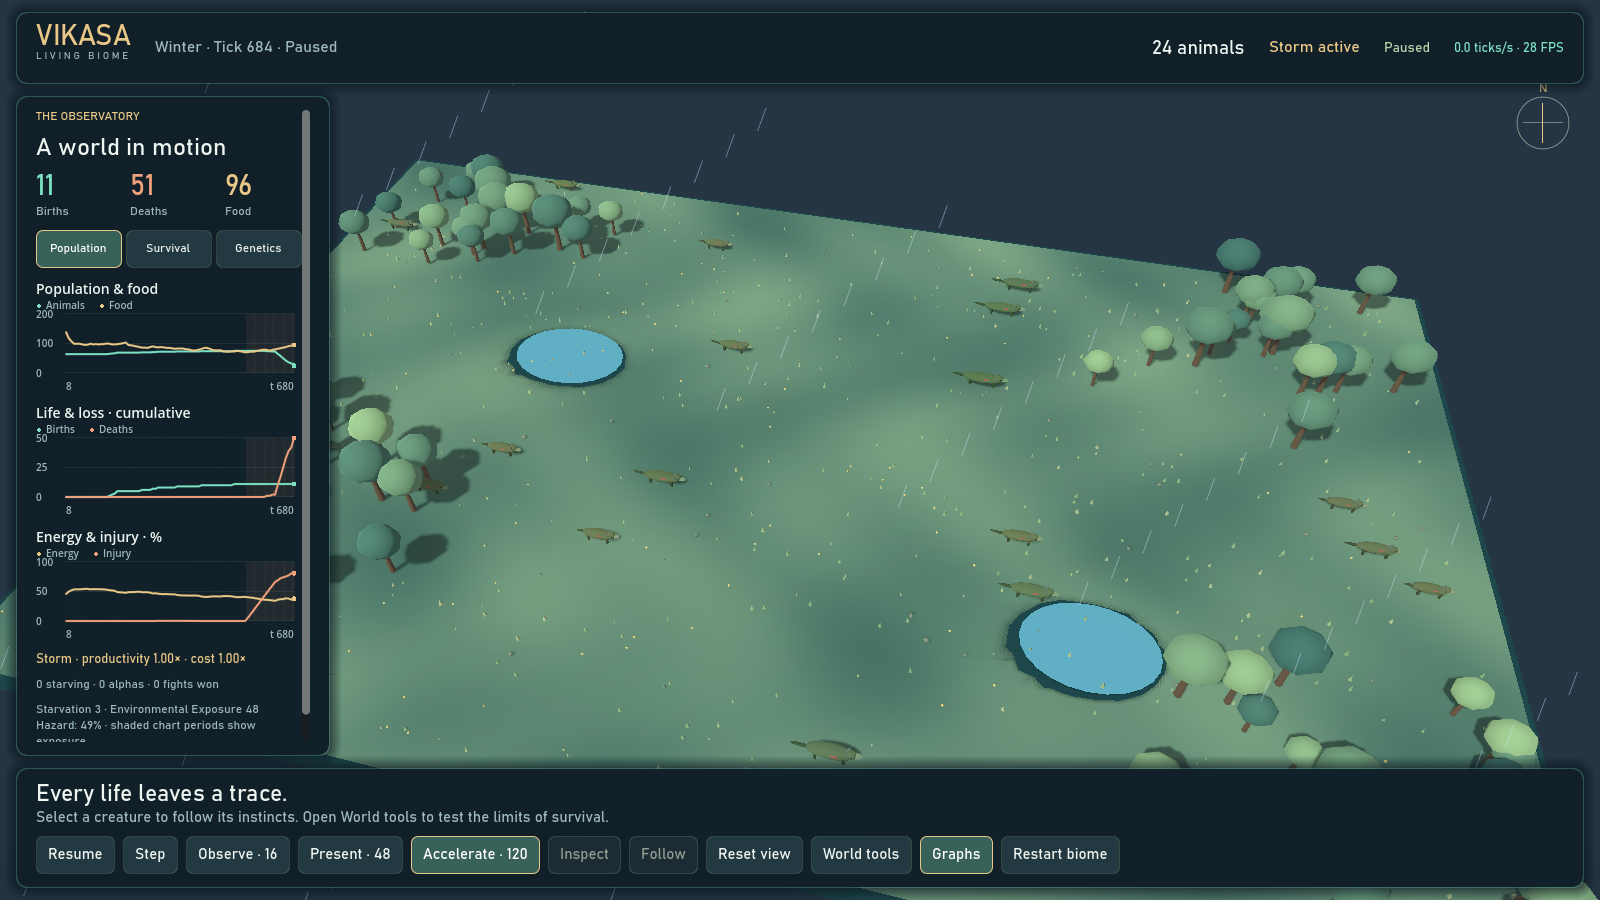
\includegraphics[width=0.6\textwidth]{presentation-storm.png}
\caption{An explicitly applied storm in an older showcase: exposure shading,
falling population and cause-of-death totals.}
\end{figure}

%===========================================================
\chapter{Spatial Plant--Water Ecology}
%===========================================================

The research profile \code{config/spatial-biome.json} replaces abstract food
spawning with a finite $24\times16$ plant-energy field coupled to soil-water
buckets. It is an inspectable conceptual model, not a calibrated hydrological
solver. Each cell carries plant energy $B\in[0,K]$ and dimensionless water
$W\in[0,1]$.

\section{Growth}
Rain first fills available bucket space and evaporation removes only available
water. Local growth is an \emph{exact} logistic step,
\begin{align*}
r_{\text{loc}}&=r\cdot\text{food\_pressure}\cdot\text{seasonal\_productivity}\cdot e^{-((T-0.6)/0.35)^2}\cdot\frac{W}{h+W},\\
B_{\text{growth}}&=\frac{KB}{B+(K-B)e^{-r_{\text{loc}}}}-B,\qquad
\text{water\_used}=\text{transpiration}\cdot B_{\text{growth}}/K,
\end{align*}
limited to what available water can support. Dead cells do not grow and recover
only by transport. Weather removes a fraction $1-e^{-\text{decay}}$ of plant energy.

\section{Transport}
Water and plants undergo a conservative five-point step,
\[
X'=(1-4d)X+d\,(X_N+X_S+X_E+X_W),\qquad 0\le d\le\tfrac14,
\]
a convex combination that preserves non-negativity and maxima. Collision worlds
replicate edges (no flux); wrap worlds use periodic neighbours. Both conserve mass.

\section{Food transfer and audited ledgers}
Natural patch placement picks an eligible cell weighted by plant energy, subtracts
exactly the patch energy and places the patch in that cell; sparse vegetation
yields smaller patches. Cells keep a 1\% seed reservoir, and a 1-unit minimum
transfer bounds negligible fragments. Two identities are audited every run:
\begin{align*}
\text{initial plants}+\text{growth}-\text{weather loss}-\text{harvest}&=\text{current plants},\\
\text{initial water}+\text{infiltrated rain}-\text{evaporation}-\text{transpiration}&=\text{current water}.
\end{align*}
Intentional provisioning is recorded separately as \code{external\_food\_energy}
with an intervention entry (the latest 256 persist). With rainfall 0.004 and no
transpiration or saturation, one 384-tick seasonal cycle adds exactly 0.05952
water per cell; the earlier 0.003 setting lost 0.15936 per cycle.

\begin{figure}[htbp]
\centering
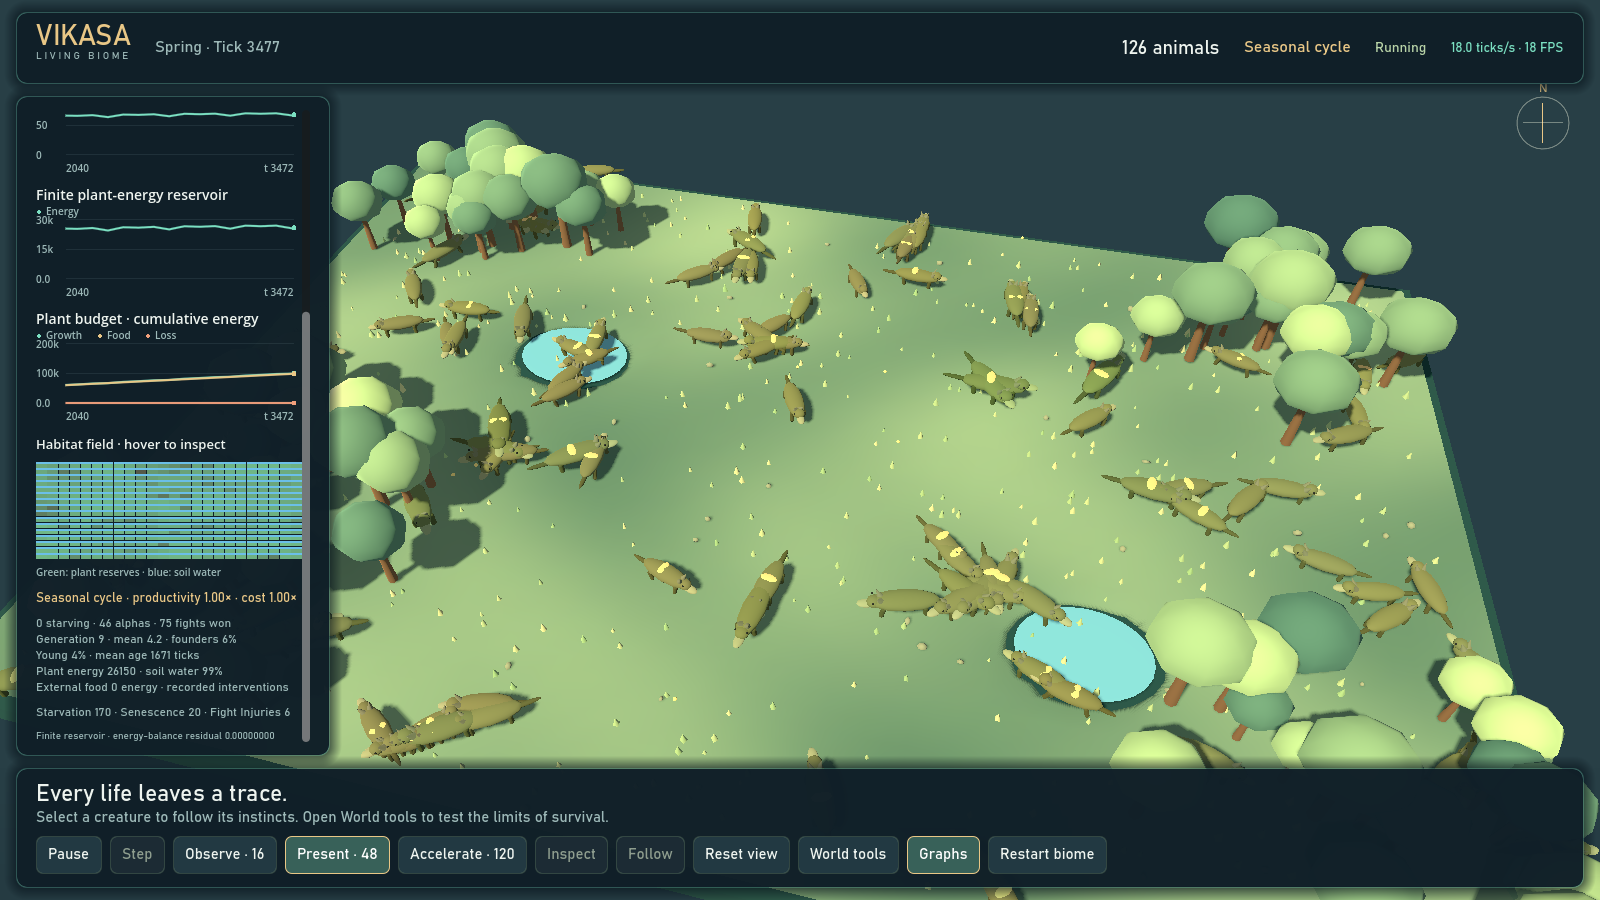
\includegraphics[width=0.9\textwidth]{spatial-ecology.png}
\caption{Ecology tab: plant/water fractions, finite plant reserves, cumulative
growth/harvest/loss, and the interactive cell map (real seed-2026 run).}
\end{figure}

\begin{table}[htbp]
\centering
\caption{Spatial study, 6{,}000 ticks, no rescue or restart}
\begin{tabular}{lcccc}
\toprule
Seed & Living & Births & Deaths & Deepest living generation \\
\midrule
2026 & 131 & 448 & 381 & 16 \\
7 & 130 & 374 & 308 & 11 \\
41 & 129 & 362 & 297 & 12 \\
\bottomrule
\end{tabular}
\end{table}
All three runs survived with no invariant failures; the 95\% Wilson survival
interval is $[0.4385,1.0000]$. Three selected seeds do not establish indefinite
survival or adaptation.

%===========================================================
\chapter{Analytics and Evolutionary Observers}
%===========================================================

Observers measure the world without changing it: none consumes engine RNG and
none runs inside decision logic. They are what turn a moving picture into
evidence.

\section{Sampled metrics}
\code{MetricsRecorder} samples the population every \code{sample\_interval}
ticks: counts of animals and food patches, cumulative births and deaths, mean
energy and injury, environmental signals, food and metabolic multipliers, trait
means, a normalised diversity summary over a sample of \code{diversity\_sample}
animals, and development measures (deepest and mean living generation, founder
fraction, juvenile fraction, mean age). Missing measurements in older saves remain
\code{null} and are drawn as gaps, never as zero.

\section{Generation depth}
Generation is \emph{ancestral depth}, not a temporal cohort. An animal with no
recorded parents is generation 0; otherwise
\[
\text{gen}(x)=1+\max\big(\text{gen}(p_1),\text{gen}(p_2)\big).
\]
\code{LineageStore.generation\_of} traverses ancestry iteratively with cycle
detection and caches results; defining a new child invalidates only that child and
its descendants. Ancestry survives the deaths of ancestors and checkpoint restore.
The deepest living generation can fall when the deepest descendant dies.

\section{Exact birth-event Price decomposition}
At every birth event the recorder observes the entire pre-birth living population
of $n$ animals. For a trait $z_i$, let $w_i$ be the attributable offspring
contribution (0.5 per child for each parent, 0 for non-parents) and $z'_i$ the
weighted mean of its descendants' trait. Then
\begin{align*}
\text{selection}&=\mathrm{Cov}(w,z)/\bar w, &
\text{transmission}&=\overline{w(z'-z)}/\bar w,\\
\text{total change}&=\textstyle\sum w z'/\sum w-\bar z, &
\text{residual}&=\text{total}-\text{selection}-\text{transmission}.
\end{align*}
Each offspring is counted once overall despite two parents. The identity is exact
to floating-point rounding. Worked example: $z=(1,3)$, $w=(1,3)$, $z'=(2,4)$ gives
$\bar w=2$, $\bar z=2$, $\mathrm{Cov}(w,z)=1$, selection $0.5$, transmission
$(1\cdot1+3\cdot1)/2/2=1.0$ and total $(2+12)/4-2=1.5$. If total descendant weight
is zero, change is undefined rather than zero. The terms are birth-event
accounting, not a causal estimate: mutation, crossover and mate choice all
contribute, and survival between births is not included. The GUI keeps 180 recent
cohorts; checkpoints and \code{evolution.json} keep 512.

\begin{figure}[htbp]
\centering
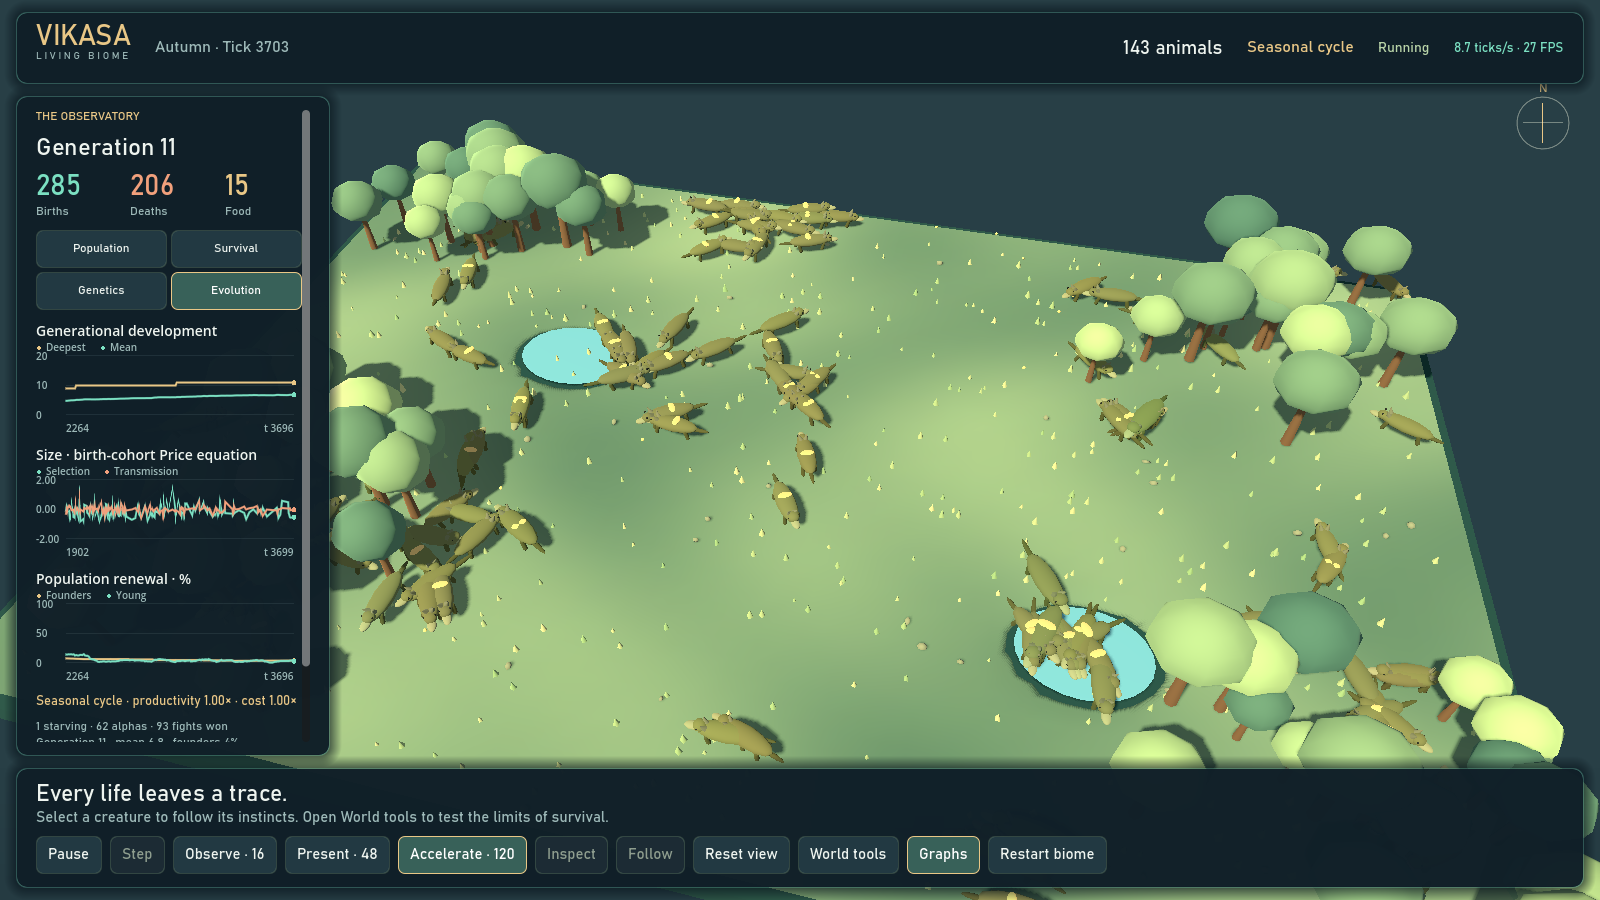
\includegraphics[width=0.92\textwidth]{research-evolution.png}
\caption{Evolution tab: generational development, signed birth-cohort Price
decomposition for size, and population renewal (founder and young fractions).}
\end{figure}

\section{Trait geometry}
At export, \code{analytics/trait\_space.py} normalises the living population's
traits to their fixed configured spans and computes
\begin{align*}
x_{ij}&=(z_{ij}-a_j)/(b_j-a_j), &
C&=(X-\bar X)^\top(X-\bar X)/(n-1),\\
R_{ij}&=C_{ij}/\sqrt{C_{ii}C_{jj}}, &
C\mathbf{v}_k&=\lambda_k\mathbf{v}_k,\quad f_k=\lambda_k/\textstyle\sum\lambda,\\
D_{\text{eff}}&=1/\textstyle\sum_k f_k^2 &&\text{(participation ratio, 1 to 6).}
\end{align*}
Eigenvectors come from NumPy \code{eigh}, sorted by descending variance, with signs
chosen so the largest-magnitude loading is positive; repeated eigenvalues are
flagged because tied axes have no unique orientation. Covariance and PCA are
unavailable below two individuals, constant columns have undefined correlations,
and non-finite or out-of-bounds clouds are rejected. $C$ is a phenotypic sample
covariance, not an additive genetic $G$ matrix, and each snapshot fits its own PCA
basis, so coordinates from different snapshots must not be connected.

\begin{figure}[htbp]
\centering
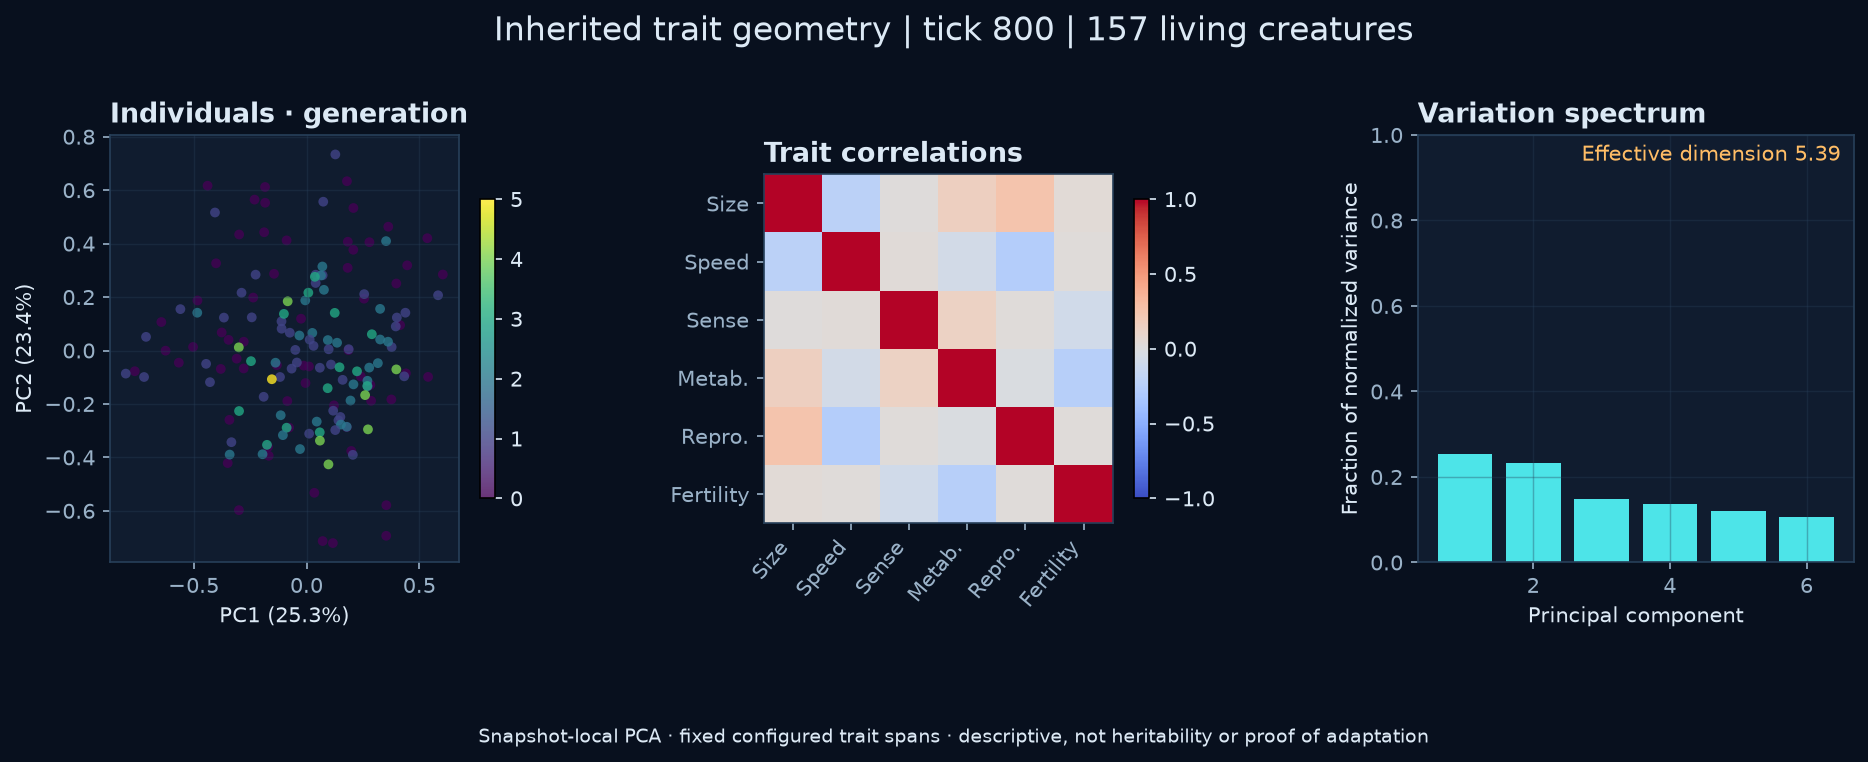
\includegraphics[width=0.95\textwidth]{trait-geometry.png}
\caption{Trait geometry, showcase seed 2026 at tick 800 (157 animals, deepest
generation 5): individuals on PC1/PC2 coloured by generation, trait correlations,
and the variance spectrum.}
\end{figure}

\section{Exported figures and how to read them}
\code{vikasa run} and \code{batch} write five static figures per run.

\begin{figure}[htbp]
\centering
\begin{minipage}{0.49\textwidth}\centering
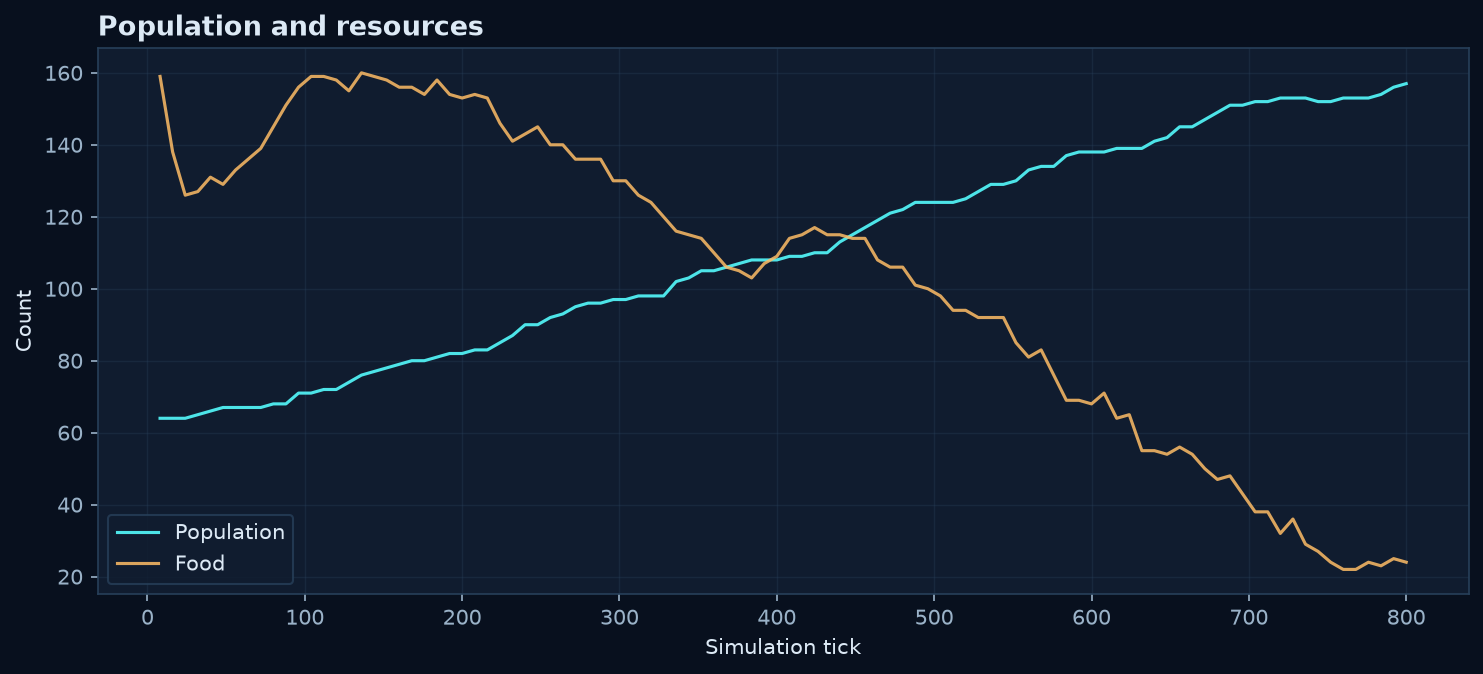
\includegraphics[width=\linewidth]{population.png}\\[-2pt]
{\small (a) Population and food patches}
\end{minipage}\hfill
\begin{minipage}{0.49\textwidth}\centering
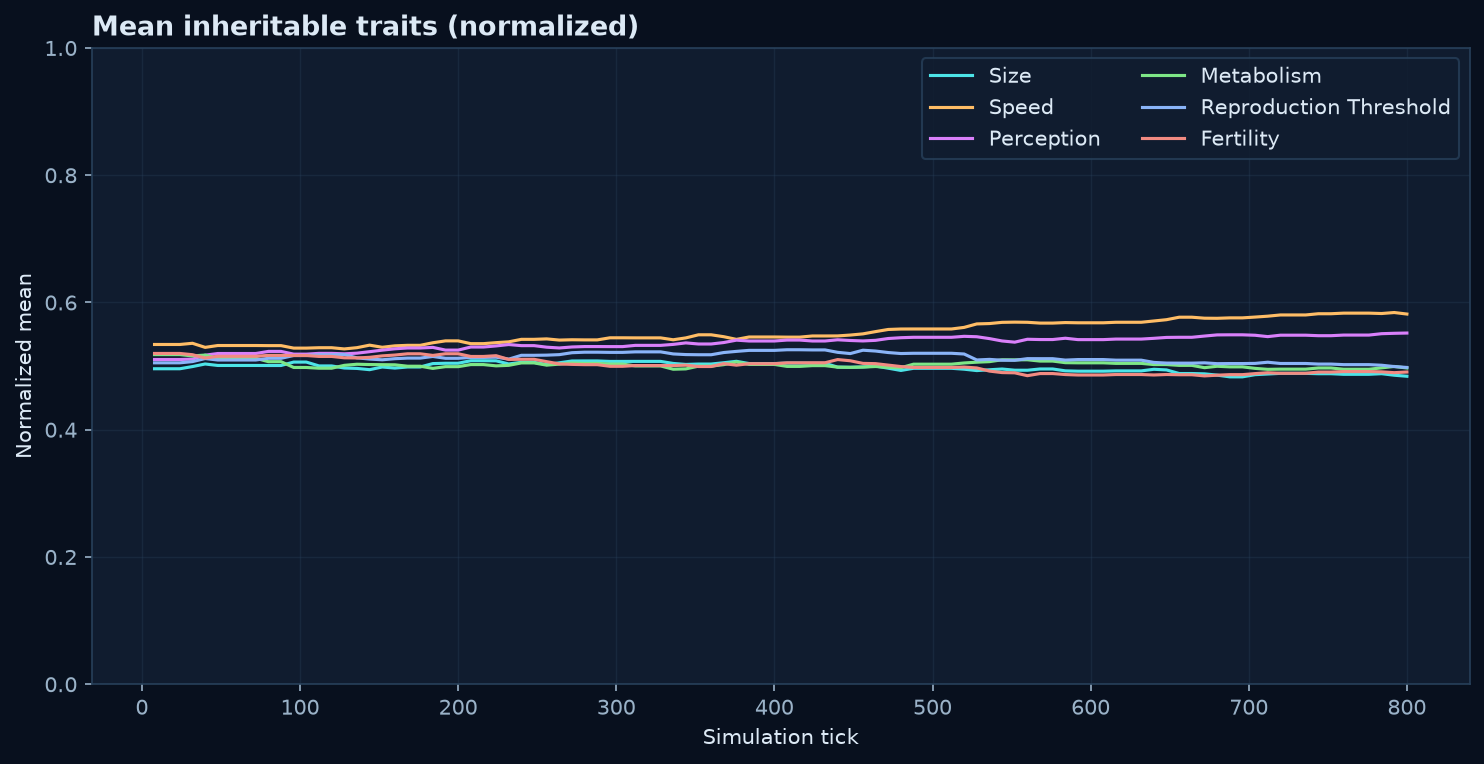
\includegraphics[width=\linewidth]{traits.png}\\[-2pt]
{\small (b) Normalised mean traits}
\end{minipage}\\[6pt]
\begin{minipage}{0.49\textwidth}\centering
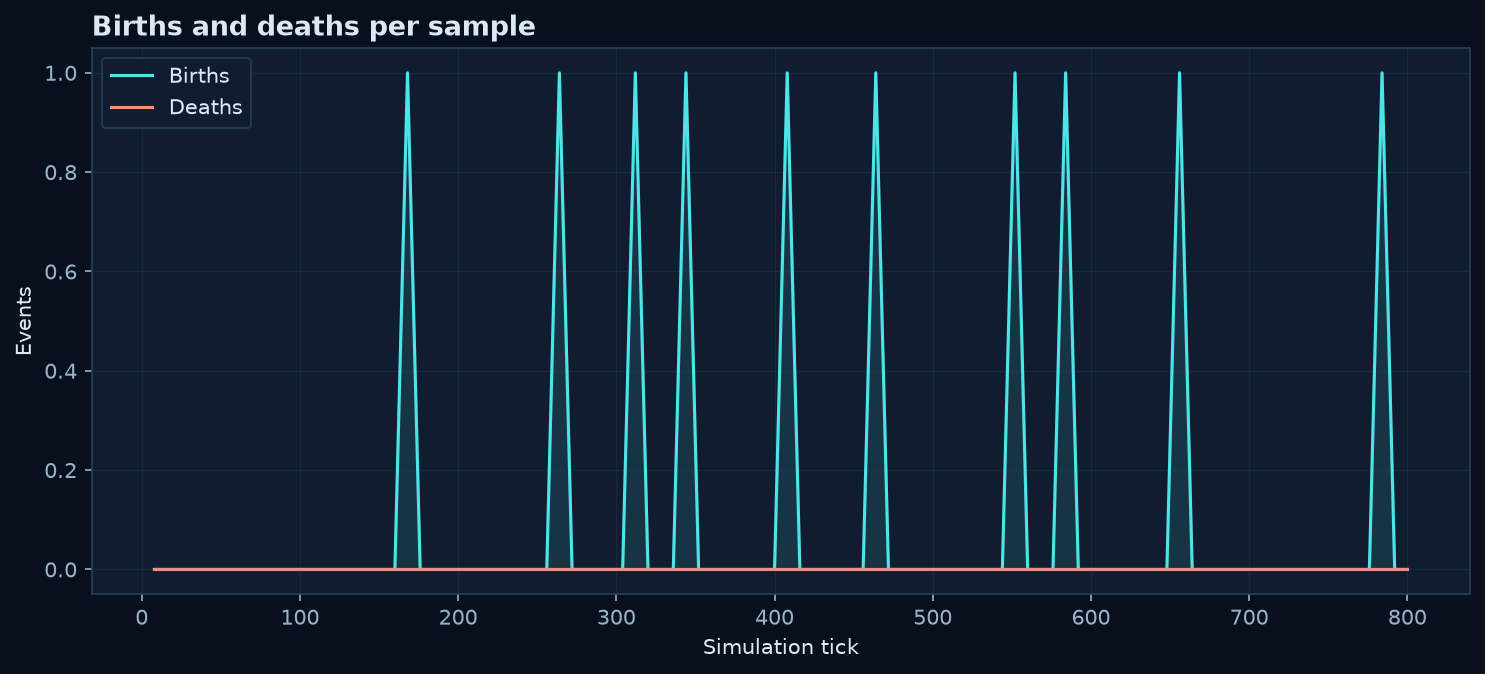
\includegraphics[width=\linewidth]{births_deaths.png}\\[-2pt]
{\small (c) Births and deaths at sample ticks}
\end{minipage}\hfill
\begin{minipage}{0.49\textwidth}\centering
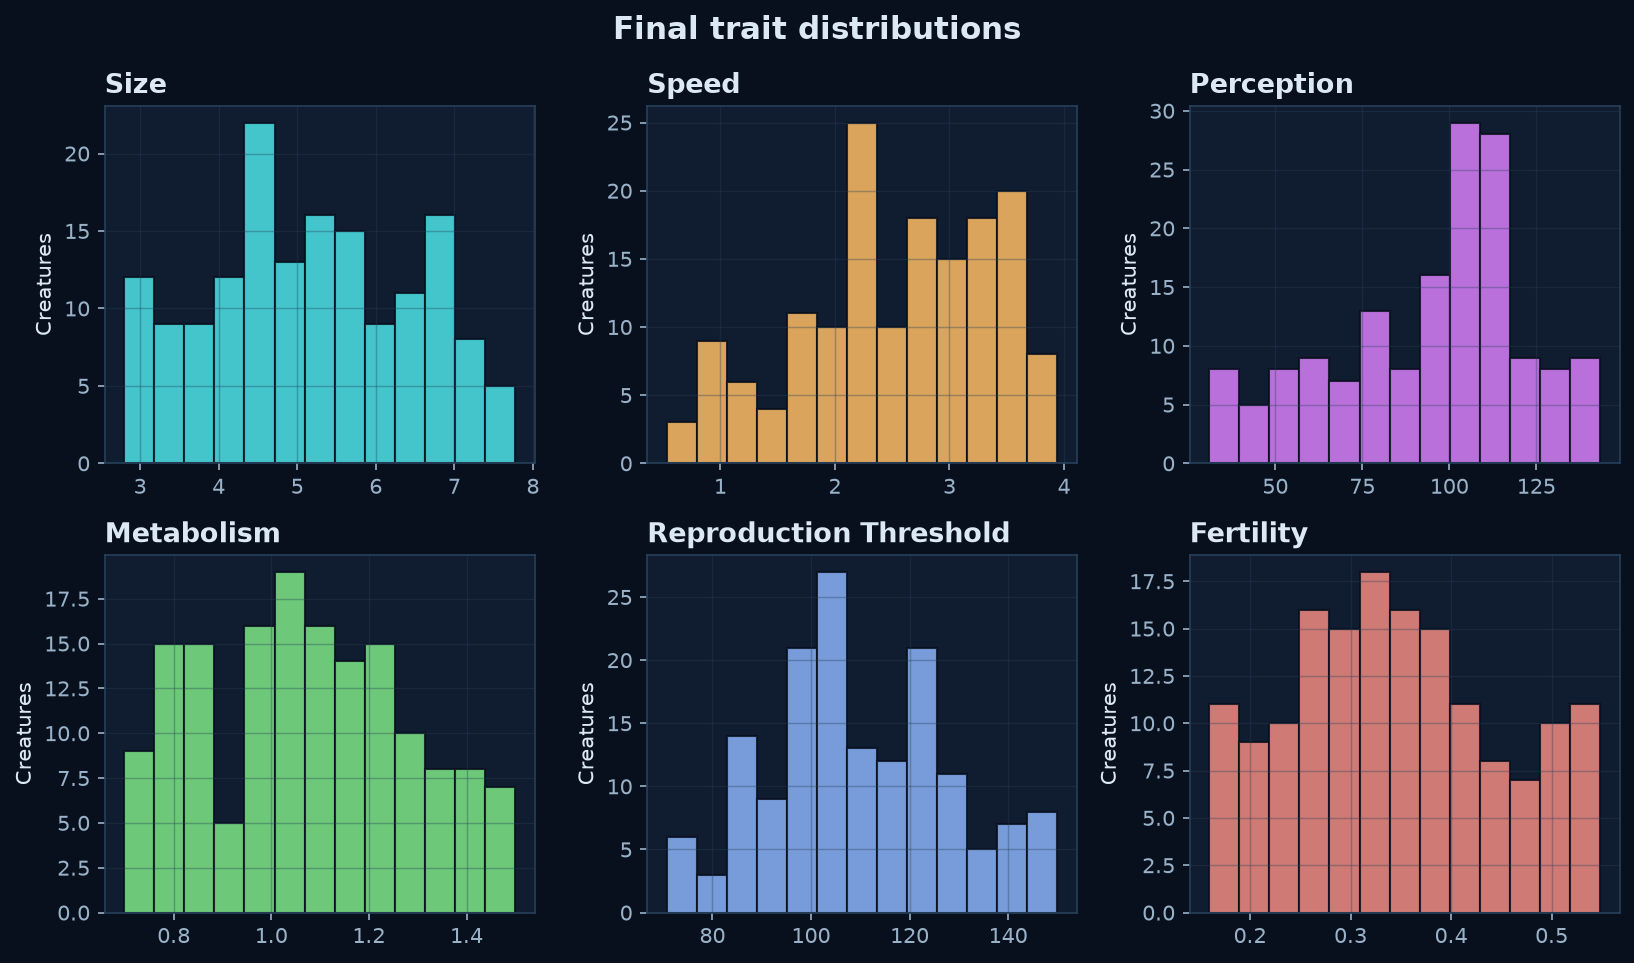
\includegraphics[width=\linewidth]{distributions.png}\\[-2pt]
{\small (d) Final trait distributions}
\end{minipage}
\caption{Exported figures for one showcase snapshot (seed 2026, tick 800).}
\end{figure}

\begin{itemize}[leftmargin=*]
\item \textbf{Ticks} are engine steps, not seconds. Requested speed is a target;
actual speed depends on hardware and population.
\item \textbf{Food-patch count} is not food energy or plant biomass.
\item \textbf{Normalised traits} $0.8$ mean 80\% through the configured range, not
80\% fitness; physical units differ between traits.
\item \textbf{Living-population means} change with births and deaths as well as
inheritance; a rising line alone does not prove adaptation.
\item \textbf{Births/deaths} in exported traces are events at the recorded sample
tick, not cumulative totals; use \code{total\_births} and \code{total\_deaths} in
the summary. For a closed run, $\text{living}=\text{founders}+\text{births}-\text{deaths}$.
\item \textbf{Weather shading} marks exposure, not proof of causation.
\item \textbf{Ribbons} in the experiment viewer are between-seed quartiles, not
confidence intervals.
\end{itemize}

\begin{table}[htbp]
\centering
\caption{Live Observatory graph groups}
\begin{tabularx}{\textwidth}{lL}
\toprule
Graph & Axes and interpretation \\
\midrule
Population \& food & Tick vs counts of animals and food patches. \\
Life \& loss (cumulative) & All births and deaths since the run began; never decrease within a run. \\
Energy \& injury & Population-mean reserve fraction and injury, as percentages. \\
Temperature \& rainfall & Normalised environmental indices (not $^{\circ}$C or mm, unless climate forcing is on). \\
Food \& metabolic pressure & Multipliers: food below $1\times$ reduces production; cost above $1\times$ raises expenditure. \\
Inherited size \& speed & Raw trait means; compare each line with itself. \\
Genetic diversity & Normalised summary of trait variation; not heterozygosity or heritability. \\
Evolution & Generation depth, renewal, signed Price terms per cohort. \\
Ecology & Plant/water fractions, reserves, cumulative flows and the cell map (spatial profile). \\
\bottomrule
\end{tabularx}
\end{table}

\section{Survival uncertainty: the Wilson interval}
For $k$ non-extinct runs out of $n$ seeds at a declared horizon, Vikasa reports
$p=k/n$ with a Wilson score interval ($z=1.959963984540054$):
\[
c=\frac{p+z^2/2n}{1+z^2/n},\qquad
h=\frac{z\sqrt{p(1-p)/n+z^2/4n^2}}{1+z^2/n},\qquad
[\max(0,c-h),\ \min(1,c+h)].
\]
This avoids reporting zero uncertainty when all of a few runs survive or die. For
$k=n=3$ it gives $[0.4385,1.0000]$, which is why three-seed studies are described
as exploratory throughout.

%===========================================================
\chapter{Headless Experiments and the Controlled Laboratory}
\label{ch:experiments}
%===========================================================

\section{Commands}
\begin{table}[htbp]
\centering
\caption{Headless science commands}
\begin{tabularx}{\textwidth}{lL}
\toprule
Command & Purpose \\
\midrule
\code{validate --config F} & Parse and validate a configuration. \\
\code{run --scenario S --output D [--seed --ticks]} & One scenario; CSV/JSON/PNG exports with hashes. \\
\code{batch --scenario S --output D --replicates 3} & Deterministic replicates with consecutive seeds. \\
\code{study --config F --seeds 2026 7 41 --ticks 12000} & Generational development study with Wilson interval. \\
\code{contrast --protocol P --output D} & Predeclared seed-blocked multi-condition comparison. \\
\code{stress --config F --ticks 100000 --seed 2026} & Long invariant-audited run. \\
\bottomrule
\end{tabularx}
\end{table}

An export directory contains \code{config.json}, \code{summary.json},
\code{metrics.csv}, \code{events.json}, \code{creatures.csv} (with generation
depth), \code{lineage.csv}, \code{evolution.json} (last 512 cohorts),
\code{trait-space.json}, \code{habitat.json} (spatial profile) and the figures
\code{population.png}, \code{traits.png}, \code{births\_deaths.png},
\code{distributions.png} and \code{trait\_space.png} (plus \code{chromosomes.png}
for diploid runs); every file's SHA-256 is recorded in the export manifest. A batch
writes one directory per replicate, \code{replicate-001-seed-<seed>}, using
consecutive seeds starting from the scenario seed.

\section{Development studies}
The \code{study} command records every selected seed, exact extinction times,
sampled trajectories, invariant errors, source and configuration hashes and a
Wilson survival interval. It never discards extinct runs, and it rejects
publication if source files change during execution.

\begin{table}[htbp]
\centering
\caption{Showcase development study, 12{,}000 ticks}
\begin{tabular}{lccccc}
\toprule
Seed & Living & Births & Living depth & \multicolumn{2}{c}{Deaths: starvation / senescence / fights} \\
\midrule
2026 & 123 & 799 & 23 & \multicolumn{2}{c}{560 / 142 / 38} \\
7 & 117 & 720 & 23 & \multicolumn{2}{c}{478 / 154 / 35} \\
41 & 114 & 717 & 20 & \multicolumn{2}{c}{477 / 158 / 32} \\
\bottomrule
\end{tabular}
\end{table}
All three passed invariant checks (Wilson $[0.4385,1.0000]$). The preserved
extinction control died out at ticks 2{,}870, 2{,}589 and 2{,}265 (Wilson
$[0.0000,0.5615]$). This is a multi-parameter comparison, not a causal estimate for
any single coefficient.

\section{Seed-blocked contrast protocol}
A contrast protocol declares a base configuration, the complete unique seed list,
horizon, sample interval, control identifier, bootstrap seed and resample count,
and every condition's overrides and events. Everything is validated before the
first tick: unknown fields, fractional or boolean seeds and times, duplicate IDs and
out-of-horizon events are rejected. Limits: 128 seeds, 8 conditions, $10^6$ ticks,
64 events per condition, 50{,}000 resamples and 250{,}000 stored records.

Extinction is absorbing, but plant and water processes continue to the same
horizon, so final water is never compared across different times. Failed runs keep
their condition, seed, stage, tick and exception, invalidate the affected
comparison, and make the CLI exit with status 1.

\subsection{Mathematics}
For condition $a$, control $c$, seed block $s$ and horizon $T$, with $N_{as}(t)$
the population after $t$ transitions:
\begin{align*}
I_{as}&=\textstyle\sum_{t=1}^{T}N_{as}(t)\ \text{[animal-ticks]}, &
M_{as}&=I_{as}/T,\\
D_s&=Y_{as}-Y_{cs}, &
\bar D&=\tfrac1n\textstyle\sum_s D_s,\\
s^2&=\tfrac{1}{n-1}\textstyle\sum_s(D_s-\bar D)^2, &
\mathrm{SE}&=\sqrt{s^2/n}.
\end{align*}
The seed block is the unit of replication. The paired bootstrap draws $n$ seed
indices with replacement, applies the same indices to both arms, and reports the
2.5th and 97.5th percentiles of the resampled means; a separate generator with the
declared bootstrap seed ensures it cannot alter biology. Hand-checked fixture: one
founder dying on transition 3 over 20 ticks has integral 2 and mean 0.1;
differences $[-2,0,2]$ give mean 0, variance 4 and SE $\sqrt{4/3}$.

\subsection{Evidence package}
Each run publishes \code{report.json}, an offline interactive \code{index.html}
(no network, no CDN, text inserted as text) and \code{manifest.json} with SHA-256
hashes. Output directories are claimed exclusively and \code{INCOMPLETE.txt} remains
until publication finishes. \code{.gitattributes} keeps LF endings so Windows
checkouts cannot invalidate byte hashes.

\begin{figure}[htbp]
\centering
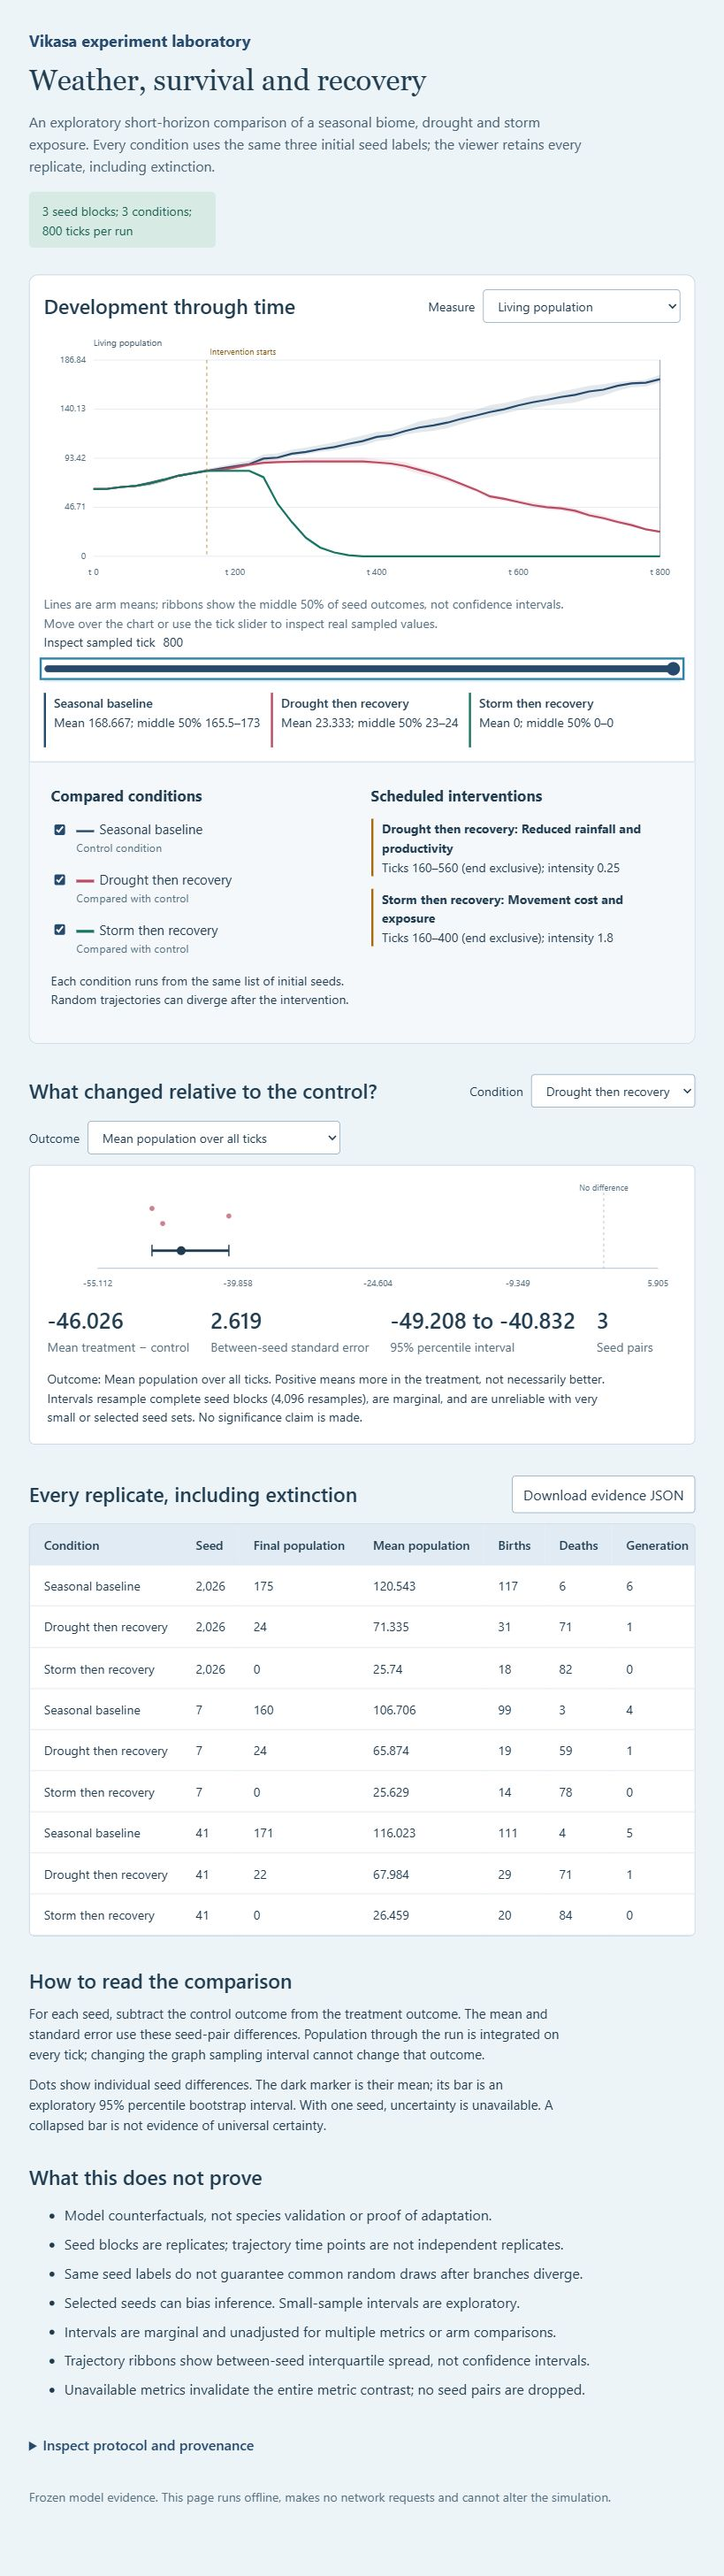
\includegraphics[width=0.9\textwidth]{controlled-experiments.jpg}
\caption{Offline weather-laboratory viewer: condition means with between-seed
quartile ribbons, intervention markers and paired effects.}
\end{figure}

\begin{table}[htbp]
\centering
\caption{Weather preview: 3 seeds $\times$ 3 conditions, 800 ticks}
\begin{tabular}{llcccc}
\toprule
Seed & Condition & Final population & Deaths & Deepest gen. & Extinction tick \\
\midrule
2026 & Baseline & 175 & 6 & 6 & --- \\
2026 & Drought & 24 & 71 & 1 & --- \\
2026 & Storm & 0 & 82 & 0 & 369 \\
7 & Baseline & 160 & 3 & 4 & --- \\
7 & Drought & 24 & 59 & 1 & --- \\
7 & Storm & 0 & 78 & 0 & 370 \\
41 & Baseline & 171 & 4 & 5 & --- \\
41 & Drought & 22 & 71 & 1 & --- \\
41 & Storm & 0 & 84 & 0 & 348 \\
\bottomrule
\end{tabular}
\end{table}
Relative to control, mean population over all ticks changed by $-46.026$ animals for
drought (paired percentile interval $[-49.208,-40.832]$) and $-88.481$ for storm
($[-94.803,-81.078]$). Storm intensity 1.8 is a severe model parameter bundle, not
a physical storm category, and drought changes rainfall, productivity, decay,
metabolism and exposure together, so the comparison estimates the configured
bundle, not an isolated mechanism. A larger eight-seed, 3{,}000-tick protocol
(\code{experiments/weather-contrast.json}) is provided for prospective execution.

%===========================================================
\chapter{Climate Rescue: Can Evolution Outrun Warming?}
\label{ch:climate}
%===========================================================

\note{Climate forcing is observed data; the organism is a generic model, not a
calibrated real species.}

\section{The question and its theory}
\emph{Evolutionary rescue} is the recovery of a declining population through
adaptive genetic change (Gomulkiewicz \& Holt 1995; Bell \& Gonzalez 2009).
Quantitative-genetic theory (Lynch \& Lande 1993; B\"urger \& Lynch 1995) predicts
a critical rate of environmental change: below it the mean phenotype settles at a
constant lag behind a moving optimum; above it the lag grows until extinction. The
climate module measures that rate in Vikasa's individual-based world, then adds a
real-data climate twin, a Sobol sensitivity analysis, a Gaussian-process surrogate
and an offline HTML report with a SHA-256 manifest. The model is described here
following the ODD protocol (Grimm et al.\ 2006, 2020).

\section{ODD description}
\subsection{Purpose and patterns}
Estimate the warming rate in $^{\circ}$C per generation beyond which a population
with heritable thermal tolerance can no longer persist, and how much of persistence
is due to evolution. Expected patterns: survival falls as the rate rises;
heritability raises the tolerable rate; the evolved shift tracks warming at slow
rates; the adaptation lag grows with the rate.

\subsection{Entities, state variables and scales}
Animals carry the six body genes, temperament, energy, injury and age, plus a
thermal optimum $\theta$ ($^{\circ}$C) and current stress $\varsigma\in[0,1)$. The
environment carries $T(t)$ in $^{\circ}$C. Space is a $480\times320$ 2D world with
tens of animals; time is in ticks, and results are reported per measured generation.

\subsection{Process overview}
The ordinary Vikasa tick (Algorithm~\ref{alg:tick-doc}) runs unchanged. Thermal
stress is computed in the energy step, before the basal cost, and affects
reproduction eligibility and the cause assigned to injury deaths in the same tick.

\subsection{Design concepts}
Thermal performance is an asymmetric Gaussian (Huey \& Kingsolver 1989). With
$\Delta T=T-\theta$:
\[
\varsigma=1-\exp\!\left(-\frac{\Delta T^2}{2w^2}\right),\qquad
w=\begin{cases}0.6\,\omega&\Delta T>0\ \text{(warm side)}\\ \omega&\Delta T\le0\end{cases}
\]
The costs of stress are: basal cost $\times(1+1.5\varsigma)$; injury
$+0.02(\varsigma-0.3)/0.7$ per tick when $\varsigma>0.3$; and no breeding while
$\varsigma>0.7$ (heat-induced sterility; Walsh et al.\ 2019). Inheritance follows
the infinitesimal model (Section 6.4); the control arm has zero heritability.

\begin{figure}[htbp]
\centering
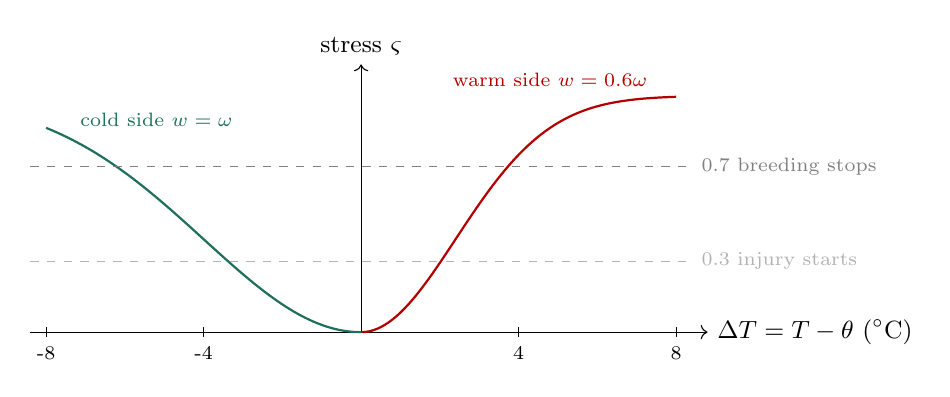
\begin{tikzpicture}
\draw[->] (-4.2,0) -- (4.4,0) node[right]{\small $\Delta T=T-\theta$ ($^{\circ}$C)};
\draw[->] (0,0) -- (0,3.4) node[above]{\small stress $\varsigma$};
\foreach \x in {-4,-2,2,4} \draw (\x,0.06)--(\x,-0.06) node[below]{\scriptsize \pgfmathparse{int(\x*2)}\pgfmathresult};
\draw[thick,vk,domain=-4:0,samples=80] plot (\x,{3*(1-exp(-(2*\x)^2/(2*16)))});
\draw[thick,red!70!black,domain=0:4,samples=80] plot (\x,{3*(1-exp(-(2*\x)^2/(2*(0.6*4)^2)))});
\draw[dashed,gray] (-4.2,2.1) -- (4.2,2.1) node[right,font=\scriptsize]{0.7 breeding stops};
\draw[dashed,gray!60] (-4.2,0.9) -- (4.2,0.9) node[right,font=\scriptsize]{0.3 injury starts};
\node[font=\scriptsize,vk] at (-2.6,2.7) {cold side $w=\omega$};
\node[font=\scriptsize,red!70!black] at (2.4,3.2) {warm side $w=0.6\omega$};
\end{tikzpicture}
\caption{Asymmetric thermal stress for $\omega=4\,^{\circ}$C. The warm side
reaches the breeding limit at $\Delta T\approx+3.7\,^{\circ}$C, the cold side only
at $\approx-6.2\,^{\circ}$C.}
\end{figure}

\subsection{Initialisation and input data}
Founders draw $\theta\sim\mathcal{N}(\bar T+\Delta_0,1\,^{\circ}\mathrm{C})$. World,
resources and population come from \code{config/climate-rescue.json}. Temperature is
\[
T(t)=T_{\text{clim}}\big(\text{month}(t)\big)+\Delta\big(\text{year}(t)\big),
\]
where $T_{\text{clim}}$ is the 1991--2020 monthly climatology of NASA POWER 2\,m
air temperature (MERRA-2 reanalysis), retrieved for 1981--2025. Each region file
stores the raw series, climatology, an OLS trend $\pm$ SE and provenance (URL,
retrieval time, SHA-256 of the response); a climatology needs at least 20 years.
The anomaly $\Delta$ is linear from 2005 (the centre of 1995--2014) to 2090 (the
centre of 2081--2100) and reaches the IPCC AR6 WG1 Chapter~4 Table~4.5 medians,
optionally multiplied by a regional factor.

\begin{table}[htbp]
\centering
\caption{IPCC AR6 warming medians and derived rates}
\begin{tabular}{lcc}
\toprule
Pathway & 2081--2100 vs 1995--2014 & Linear rate ($^{\circ}$C/yr) \\
\midrule
SSP1-2.6 & 0.9\,$^{\circ}$C & 0.011 \\
SSP2-4.5 & 1.8\,$^{\circ}$C & 0.021 \\
SSP3-7.0 & 2.8\,$^{\circ}$C & 0.033 \\
SSP5-8.5 & 3.5\,$^{\circ}$C & 0.041 \\
\bottomrule
\end{tabular}
\end{table}

\begin{table}[htbp]
\centering
\caption{Published study regions}
\begin{tabular}{lccc}
\toprule
Region & Annual mean & Seasonal amplitude & Trend 1981--2025 ($^{\circ}$C/decade) \\
\midrule
Western Ghats (Agumbe) & 25.3 & 2.4 & $+0.169\pm0.029$ \\
Delhi NCR & 25.6 & 11.1 & $-0.120\pm0.068$ \\
Sundarbans & 26.2 & 5.4 & $-0.002\pm0.030$ \\
\bottomrule
\end{tabular}
\end{table}
The slight Delhi cooling is reported as measured; it is consistent with aerosol
and haze dimming over the Indo-Gangetic plain in MERRA-2 and is not a forecast.

\subsection{Submodels and calibration}
The generation interval is $1/$slope of mean living ancestral depth per tick at
zero warming, averaged over three calibration seeds (901, 902, 903; 1{,}500
burn-in and 6{,}000 measured ticks): $G=469$ ticks. The rescue protocol has 5
generations of burn-in, 20 of warming at rate $r$ and 5 of hold, with one climate
year per generation, Western Ghats climatology and $\omega=4\,^{\circ}$C.
Outcomes: survival, extinction generation, population before warming, at minimum
and at the end, evolved shift in mean $\theta$, adaptation lag over the last five
warming generations, and the rescue signature (dip below 50\% then recovery to
$\ge80\%$). For the sweep the monthly cycle is a sinusoid whose half-range equals
the amplitude exactly.

\section{The pipeline}
\begin{lstlisting}
vikasa climate pipeline --profile full --root exports\climate\full
vikasa climate pipeline --profile quick --root exports\climate\quick
vikasa climate fetch --lat 18.52 --lon 73.86 --name Pune --key pune --output data\pune.json
vikasa climate assess --root exports\climate\full --region data\pune.json \
    --generation-years 2 --breadth 3 --ssp SSP2-4.5 --ssp SSP5-8.5
vikasa climate report --root exports\climate\full
\end{lstlisting}
The pipeline runs five resumable stages (calibrate, sweep, sensitivity, assess,
report) in parallel worker processes, appending results to JSON-lines files so an
interrupted run continues where it stopped. A root calibrated for one profile
refuses another.

\begin{table}[htbp]
\centering
\caption{Pipeline profiles}
\begin{tabularx}{\textwidth}{lLL}
\toprule
Setting & quick & full \\
\midrule
Rates ($^{\circ}$C/gen) & 0, 0.3, 1.2 & 0, 0.025, 0.05, 0.075, 0.1, 0.15, 0.2, 0.3, 0.4 \\
Seeds per cell & 3 & 12 \\
Phases (gens) & 2 / 4 / 2 & 5 / 20 / 5 \\
Calibration & 1 seed, 500 + 1{,}500 ticks & 3 seeds, 1{,}500 + 6{,}000 ticks \\
Design / hold-out points & 24 / 8 & $2\times192$ / 48 \\
Sobol $n$, bootstrap & 1{,}024, 200 & 4{,}096, 2{,}000 \\
Regions, SSPs & Western Ghats; 2 SSPs & 3 regions; 4 SSPs \\
Assessment seeds, cap & 3, 4 gens & 12, 40 gens; local breadth $1.5\times$ \\
\bottomrule
\end{tabularx}
\end{table}

\section{Statistics}
\begin{itemize}[leftmargin=*]
\item \textbf{Critical rate.} A lightly penalised logistic regression (L2, $C=10$
on the rate scaled by its maximum, L-BFGS) fits $\mathrm{logit}\,p=\beta_0+\beta_1r$,
finite even under perfect separation. $k_c=-\beta_0/\beta_1$ is accepted only if
$\beta_1<0$ and $0\le k_c\le2r_{\max}$. A 2{,}000-resample bootstrap gives the CI.
\item \textbf{Rescue gain.} Paired bootstrap over seeds of $k_c^{\text{her}}-k_c^{\text{ctl}}$.
\item \textbf{Lag regression.} Pearson correlation and slope of lag against rate over surviving heritable runs.
\item \textbf{Sensitivity.} Six inputs (Table~\ref{tab:sobolparams}) sampled by Latin
hypercube. A GP regressor with kernel $\text{Const}\times\text{Mat\'ern}_{5/2}(\ell=0.3)+\text{White}(0.01)$
models the final/pre-warming population ratio, clipped to $[0,2]$. Survival
probability is $P(\text{ratio}>\tau)$ under the predictive normal, where $\tau$ is
the midpoint between the largest extinct and smallest surviving training ratio.
Five-fold CV and hold-out $R^2$, AUC and Brier score assess it.
\item \textbf{Sobol indices.} Scrambled Sobol (Saltelli) base samples $A,B$ with
$n=4{,}096$, $AB_i$ swapping column $i$, Jansen estimators
$S_i=(V-\tfrac12\mathbb{E}[(f_B-f_{AB_i})^2])/V$ and
$S_{T,i}=\tfrac12\mathbb{E}[(f_A-f_{AB_i})^2]/V$, 200 bootstrap resamples; the
estimator is unit-tested on the Ishigami function.
\end{itemize}

\begin{table}[htbp]
\centering
\caption{Sensitivity inputs}
\label{tab:sobolparams}
\begin{tabular}{llc}
\toprule
Input & Meaning & Range \\
\midrule
\code{rate\_c\_per\_gen} & Warming rate & 0 -- $r_{\text{high}}$ \\
\code{breadth\_c} & Cold-side tolerance breadth & 2 -- 8\,$^{\circ}$C \\
\code{amplitude\_c} & Seasonal amplitude & 0.5 -- 8\,$^{\circ}$C \\
\code{founder\_sd\_c} & Standing variation in $\theta$ & 0.25 -- 2\,$^{\circ}$C \\
\code{segregation\_sd\_c} & Heritable offspring variation & 0 -- 1\,$^{\circ}$C \\
\code{capacity\_scale} & Carrying-capacity multiplier & 0.5 -- 1.5 \\
\bottomrule
\end{tabular}
\end{table}

\section{Results}
All numbers come from \code{docs/results/climate-rescue-2026-10-18/}.

\begin{table}[htbp]
\centering
\caption{Critical warming rate}
\begin{tabular}{lcc}
\toprule
Arm & $k_c$ ($^{\circ}$C/generation) & 95\% CI \\
\midrule
Heritable thermal tolerance & \textbf{0.262} & 0.234--0.291 \\
Control: same variation, no heritability & 0.067 & 0.052--0.080 \\
Rescue gain (paired bootstrap) & \textbf{+0.196} & 0.165--0.230 \\
\bottomrule
\end{tabular}
\end{table}

\begin{figure}[htbp]
\centering
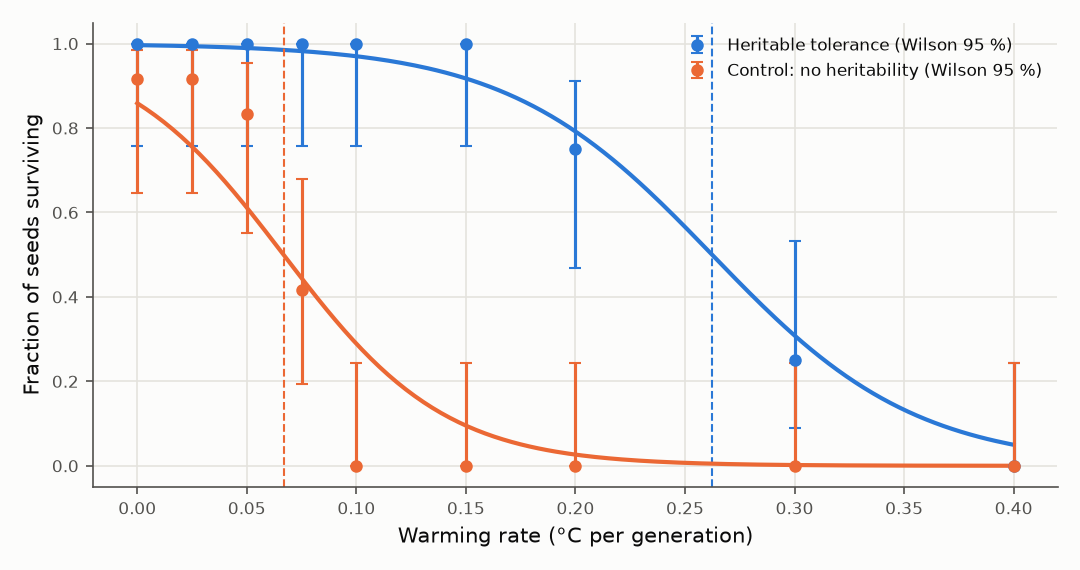
\includegraphics[width=0.82\textwidth]{survival_curve.png}
\caption{Survival against warming rate, heritable vs control, with Wilson intervals and logistic fits.}
\end{figure}

Heritable populations survived every seed up to 0.15, 9/12 at 0.2, 3/12 at 0.3
and none at 0.4\,$^{\circ}$C/gen; controls began failing at 0.075 and none
survived 0.1. The evolved shift was $+1.2$, $+2.9$ and $+4.5\,^{\circ}$C at 0.1,
0.2 and 0.3 (against 2, 4 and 6\,$^{\circ}$C of warming). Lag rose linearly with
slope 6.4\,$^{\circ}$C per ($^{\circ}$C/gen), $r=0.85$, $n=81$. Near $k_c$,
17--25\% of surviving runs showed the rescue signature.

\begin{figure}[htbp]
\centering
\begin{minipage}{0.49\textwidth}\centering
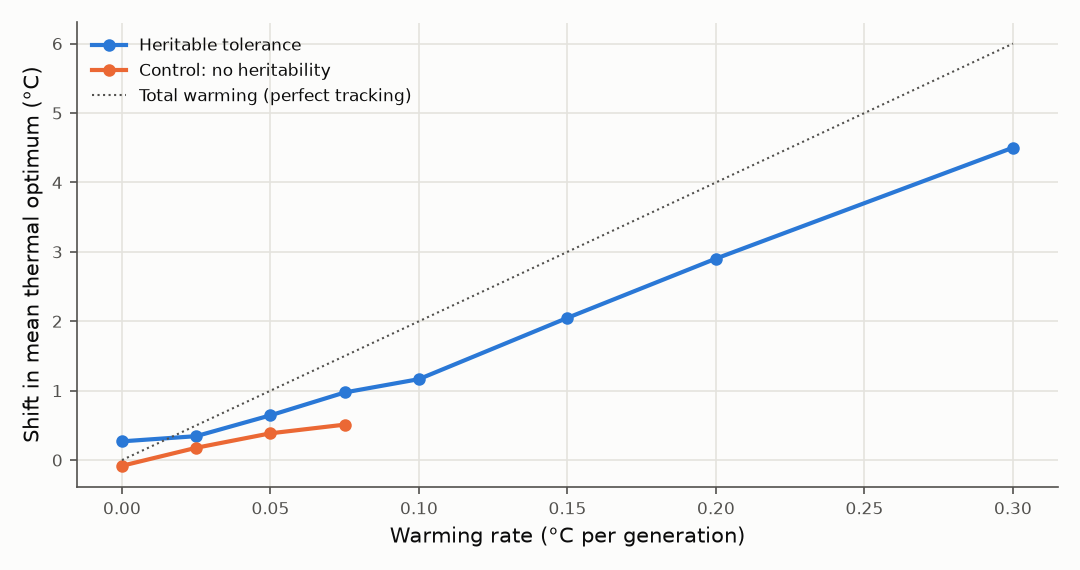
\includegraphics[width=\linewidth]{shift_vs_rate.png}\\[-2pt]
{\small (a) Evolved shift in mean optimum}
\end{minipage}\hfill
\begin{minipage}{0.49\textwidth}\centering
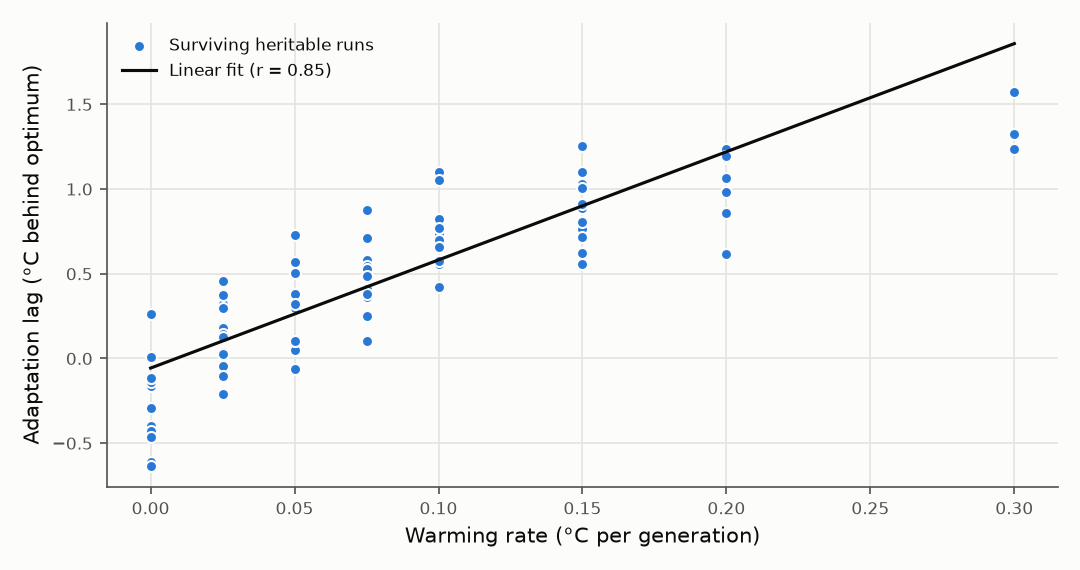
\includegraphics[width=\linewidth]{lag_vs_rate.png}\\[-2pt]
{\small (b) Adaptation lag}
\end{minipage}
\caption{Shift and lag versus warming rate.}
\end{figure}

\begin{figure}[htbp]
\centering
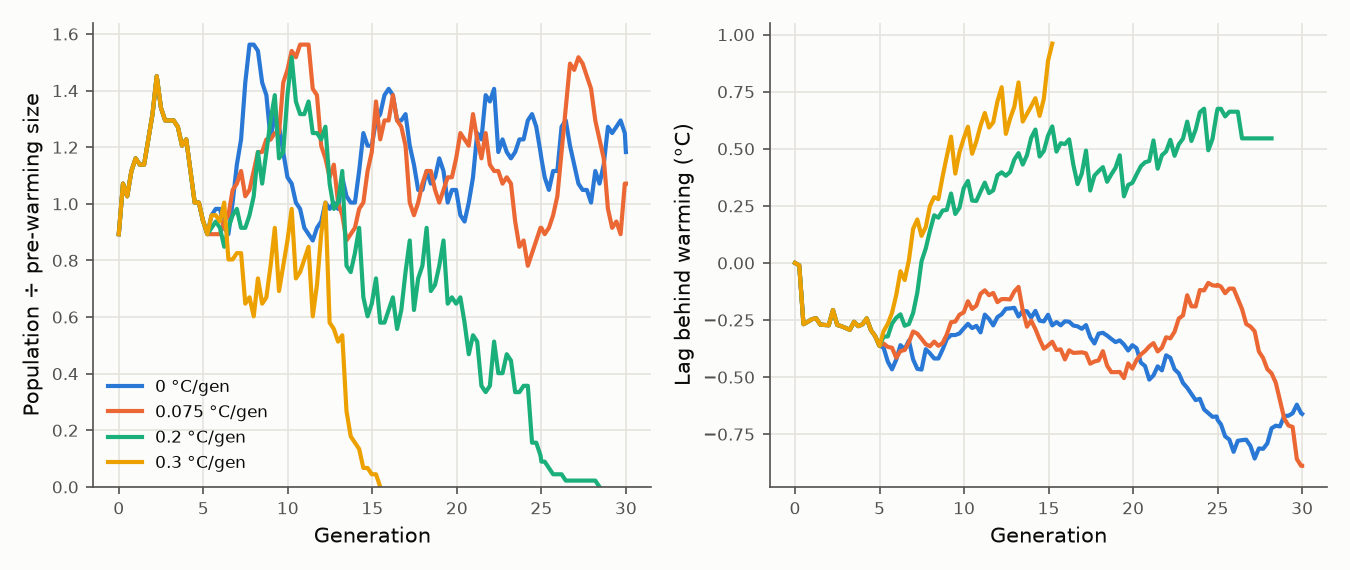
\includegraphics[width=0.95\textwidth]{trajectories.png}
\caption{Population and lag trajectories through burn-in, warming and hold.}
\end{figure}

\begin{figure}[htbp]
\centering
\begin{minipage}{0.56\textwidth}\centering
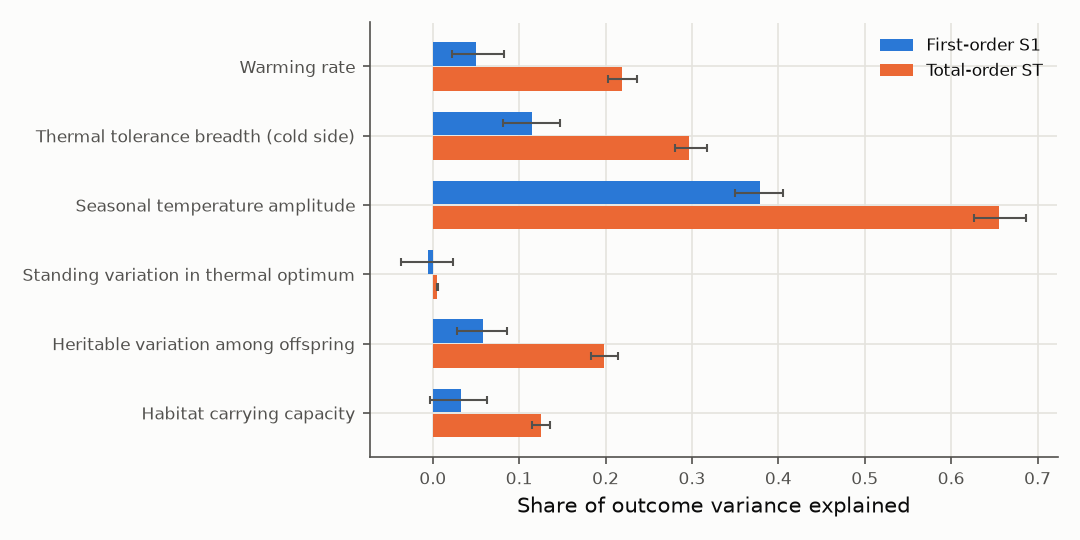
\includegraphics[width=\linewidth]{sobol_bars.png}\\[-2pt]
{\small (a) Sobol indices}
\end{minipage}\hfill
\begin{minipage}{0.4\textwidth}\centering
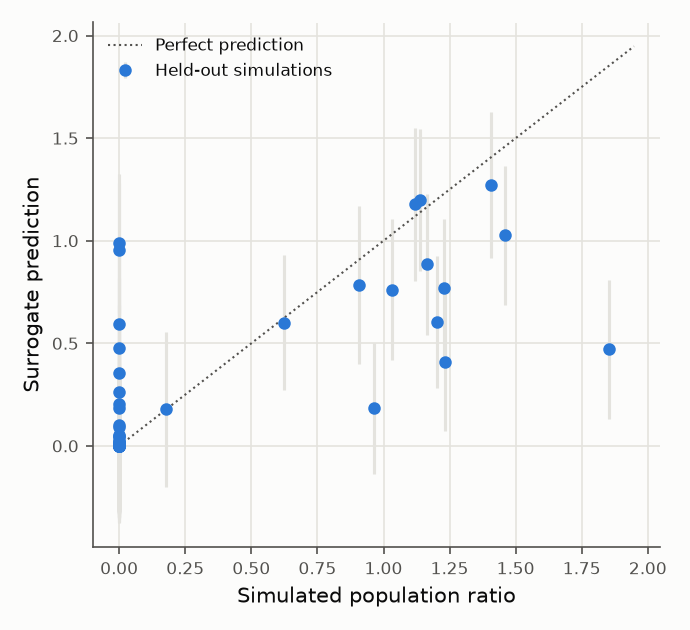
\includegraphics[width=\linewidth]{surrogate_parity.png}\\[-2pt]
{\small (b) Surrogate parity}
\end{minipage}
\caption{Sensitivity: total-order indices were amplitude 0.66, breadth 0.30, rate
0.22, segregation SD 0.20, capacity 0.13, standing variation $\approx0$.}
\end{figure}

\begin{table}[htbp]
\centering
\caption{Regional viability}
\begin{tabularx}{\textwidth}{lLL}
\toprule
Region & Reference organism ($\omega=4$) & Locally adapted ($1.5\times$ amplitude) \\
\midrule
Western Ghats & persists under all SSPs ($p=0.92$--$1.0$) & same as reference \\
Delhi NCR & not viable even without warming & $\omega=16.6$: persists, $p=0.92$--$1.0$ \\
Sundarbans & not viable even without warming & $\omega=8.2$: persists, $p=1.0$ \\
\bottomrule
\end{tabularx}
\end{table}

\begin{table}[htbp]
\centering
\caption{Critical generation time $=k_c\,/\,$warming per year}
\begin{tabular}{lcc}
\toprule
Scenario & Warming ($^{\circ}$C/yr) & Critical generation time (yr, 95\% CI) \\
\midrule
SSP1-2.6 & 0.011 & 24.8 (22.1--27.5) \\
SSP2-4.5 & 0.021 & 12.4 (11.0--13.7) \\
SSP3-7.0 & 0.033 & 8.0 (7.1--8.8) \\
SSP5-8.5 & 0.041 & 6.4 (5.7--7.1) \\
\bottomrule
\end{tabular}
\end{table}

Checked by direct simulation (Western Ghats, real monthly cycle, 2025--2100, 12
seeds): six-year species survive with $p=1.00$ (SSP2-4.5), 0.67 (SSP3-7.0) and
0.50 (SSP5-8.5, where 0.247\,$^{\circ}$C/gen $\approx k_c$); twelve-year species
0.92, 0.50 and 0.25. Twelve-year species beat the simple rule because 2025--2100
spans only about six generations, so the critical generation time is conservative
for long-lived species over this century.

\begin{figure}[htbp]
\centering
\begin{minipage}{0.49\textwidth}\centering
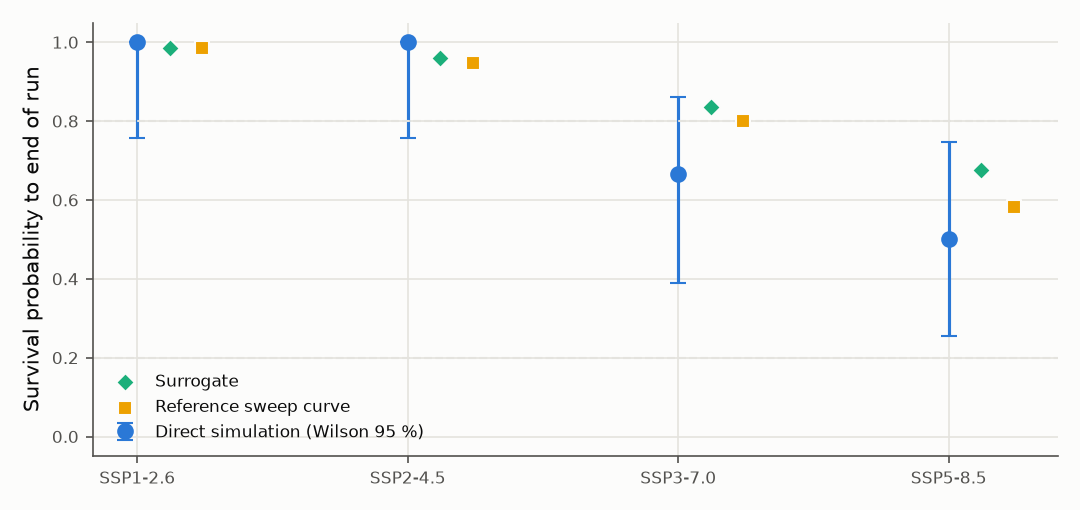
\includegraphics[width=\linewidth]{assessment_western-ghats-g6.png}\\[-2pt]
{\small (a) Six-year generations}
\end{minipage}\hfill
\begin{minipage}{0.49\textwidth}\centering
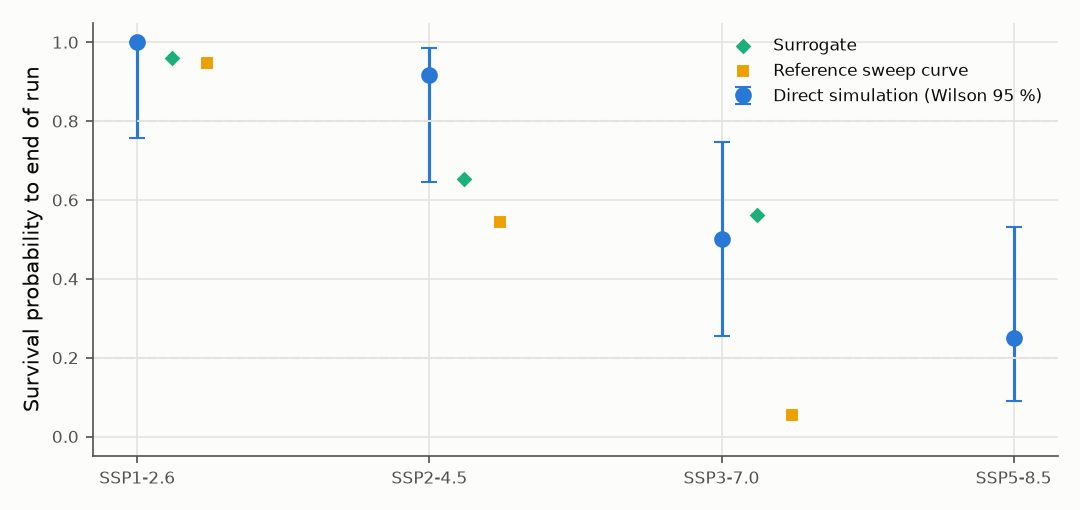
\includegraphics[width=\linewidth]{assessment_western-ghats-g12.png}\\[-2pt]
{\small (b) Twelve-year generations}
\end{minipage}
\caption{Direct regional assessments, Western Ghats.}
\end{figure}

\section{Pre-registered success criteria}
\begin{longtable}{p{0.8cm}p{1.2cm}p{12.4cm}}
\caption{Criteria fixed before the production run}\\
\toprule
ID & Result & Criterion and outcome \\
\midrule
\endfirsthead
C1 & PASS & Populations persist without warming: 12/12. \\
C2 & PASS & Faster warming lowers survival: Spearman $\rho=-0.84$. \\
C3 & PASS & Heritability raises $k_c$: gain CI 0.165--0.230. \\
C4 & FAIL & Optima track $\ge50\%$ of warming and $\ge2\times$ the control shift at $\le k_c/2$. The first holds, but controls also shift by about half as much: heat kills cold-adapted individuals within each generation, so the surviving control population's mean optimum moves although nothing is inherited. \\
C5 & PASS & Lag grows with rate: $r=0.85$. \\
C6 & PASS & No invariant violations or failed runs: 0/0. \\
S9 & FAIL & Surrogate hold-out $R^2\ge0.7$ and AUC $\ge0.85$: $R^2=0.51$, AUC $=0.93$ after the planned one-time escalation from 192 to 384 design runs. Even a perfect predictor explains at most about 78\% of single-run variance. \\
S10 & FAIL & Warming rate in the top two drivers: ranks third ($S_T=0.22$). \\
\bottomrule
\end{longtable}
No parameters were changed after the production run to make a criterion pass.

%===========================================================
\chapter{Species Risk Checker}
\label{ch:risk}
%===========================================================

\begin{figure}[htbp]
\centering
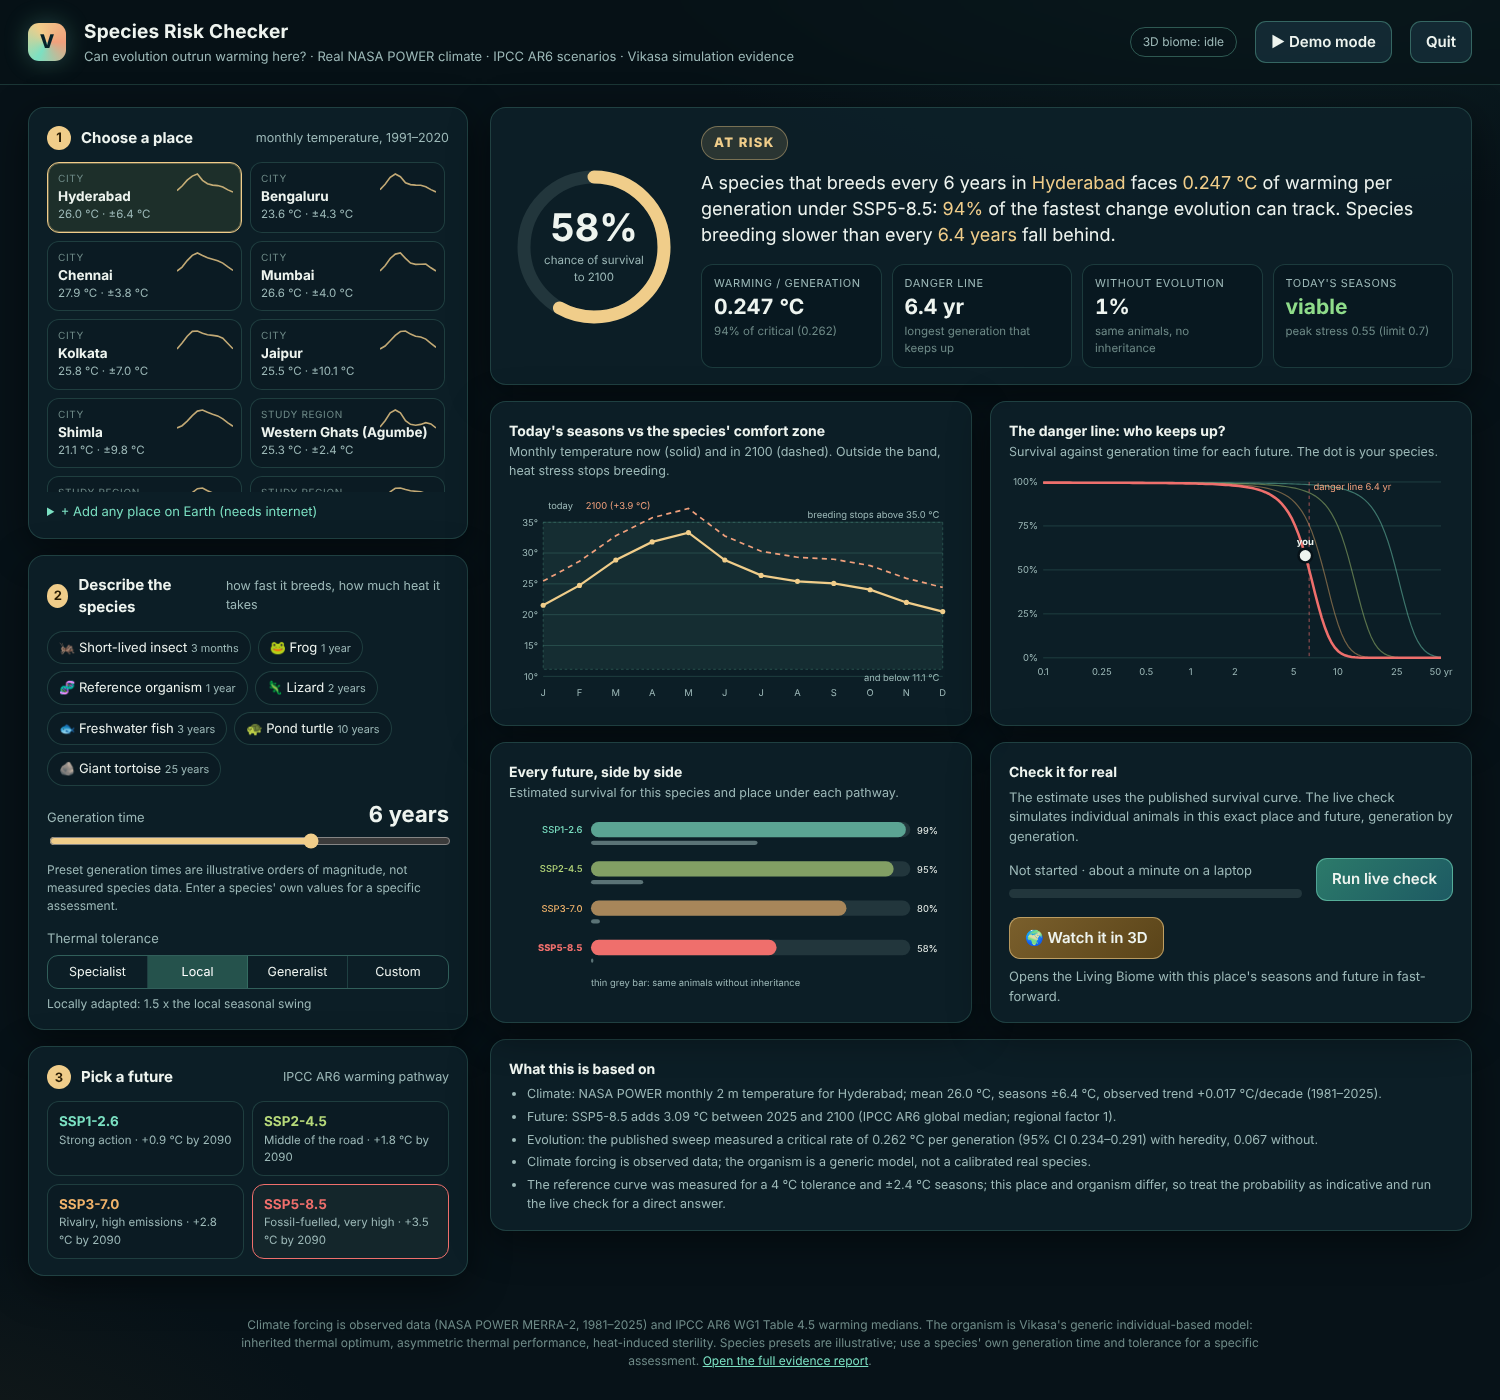
\includegraphics[width=0.5\textwidth]{risk-checker.png}
\caption{Species Risk Checker: a six-year species in Hyderabad under SSP5-8.5.}
\end{figure}

\section{Inputs}
\begin{table}[htbp]
\centering
\caption{Risk Checker inputs}
\begin{tabularx}{\textwidth}{lL}
\toprule
Input & Meaning and source \\
\midrule
Place & Monthly T2M climatology 1991--2020 and 1981--2025 trend from NASA POWER; bundled or fetched live for any latitude/longitude. \\
Generation time & Years from birth to the mean age of parents; presets from insect (3 months) to giant tortoise; range 0.05--50 years. \\
Tolerance & Breadth $\omega$: specialist $1\times$, local $1.5\times$ (default) or generalist $2.5\times$ the local seasonal swing, or a custom $^{\circ}$C value. \\
Future & SSP1-2.6, SSP2-4.5, SSP3-7.0 or SSP5-8.5. \\
\bottomrule
\end{tabularx}
\end{table}

\begin{table}[htbp]
\centering
\caption{Bundled Risk Checker places (reanalysis grid cells)}
\begin{tabular}{llccc}
\toprule
Key & Place & Mean ($^{\circ}$C) & Seasons ($\pm^{\circ}$C) & Trend ($^{\circ}$C/decade) \\
\midrule
\code{hyderabad} & Hyderabad & 26.0 & 6.4 & $+0.017$ \\
\code{bengaluru} & Bengaluru & 23.6 & 4.3 & $+0.092$ \\
\code{chennai} & Chennai & 27.9 & 3.8 & $+0.063$ \\
\code{mumbai} & Mumbai & 26.6 & 4.0 & $+0.127$ \\
\code{kolkata} & Kolkata & 25.8 & 7.0 & $-0.037$ \\
\code{jaipur} & Jaipur & 25.5 & 10.1 & $-0.075$ \\
\code{shimla} & Shimla & 21.1 & 9.8 & $-0.043$ \\
\code{western-ghats} & Western Ghats & 25.3 & 2.4 & $+0.169$ \\
\code{delhi-ncr} & Delhi NCR & 25.6 & 11.1 & $-0.120$ \\
\code{sundarbans} & Sundarbans & 26.2 & 5.4 & $-0.002$ \\
\bottomrule
\end{tabular}
\end{table}

\section{Instant estimate}
\textbf{Step 1, can it live here today?} Founders start at the annual mean; the
model's stress rule is applied to the hottest and coldest months:
\[
\varsigma_{\text{warm}}=1-e^{-(T_{\max}-\bar T)^2/2(0.6\omega)^2},\qquad
\varsigma_{\text{cold}}=1-e^{-(\bar T-T_{\min})^2/2\omega^2}.
\]
Peak stress above 0.75 is \emph{not viable}, 0.65--0.75 \emph{borderline} and below
0.65 \emph{viable}. With no fitted parameters this reproduces all five published
baseline verdicts (Western Ghats reference 0.53 viable; Sundarbans reference 0.78
not viable; Sundarbans local 0.30 viable; Delhi reference 1.00 not viable; Delhi
local 0.42 viable), enforced by
\code{test\_seasonal\_screen\_reproduces\_every\_published\_baseline\_verdict}.

\textbf{Step 2, can evolution keep up?} Warming per generation $=$ SSP rate per
year $\times$ generation time; survival with and without evolution comes from the
logistic curves stored with provenance in \code{climate/data/risk-reference.json}.
The danger line is $k_c$ divided by the warming per year.

\textbf{Domain check.} The curve was measured for $\omega=4\,^{\circ}$C and
$\pm2.4\,^{\circ}$C seasons. Inputs more than 25\% away are labelled
\emph{indicative}; rates above 0.4\,$^{\circ}$C/gen are \emph{extrapolated}.

\section{Live check and 3D replay}
\emph{Run live check} (\code{--live}) measures the generation interval in today's
climate (2 calibration seeds, 7{,}500 ticks), returns \emph{not viable in
present-day climate} if every calibration population dies, then runs 4 seeded
populations (5 burn-in, up to 25 warming, 5 hold generations) and reports survivors,
a Wilson interval and a verdict: $\ge80\%$ \emph{likely persists}, $\ge20\%$
\emph{at risk}, otherwise \emph{likely lost}. Results are cached under
\code{exports/risk/live/}. \emph{Watch it in 3D} writes a Living Biome world with
the place's real monthly cycle and the organism's breadth, applies warming each
climate year for 20 years after a 3-year settling period, and opens Godot with a
live temperature readout whose tooltip shows the adaptation lag.

\begin{figure}[htbp]
\centering
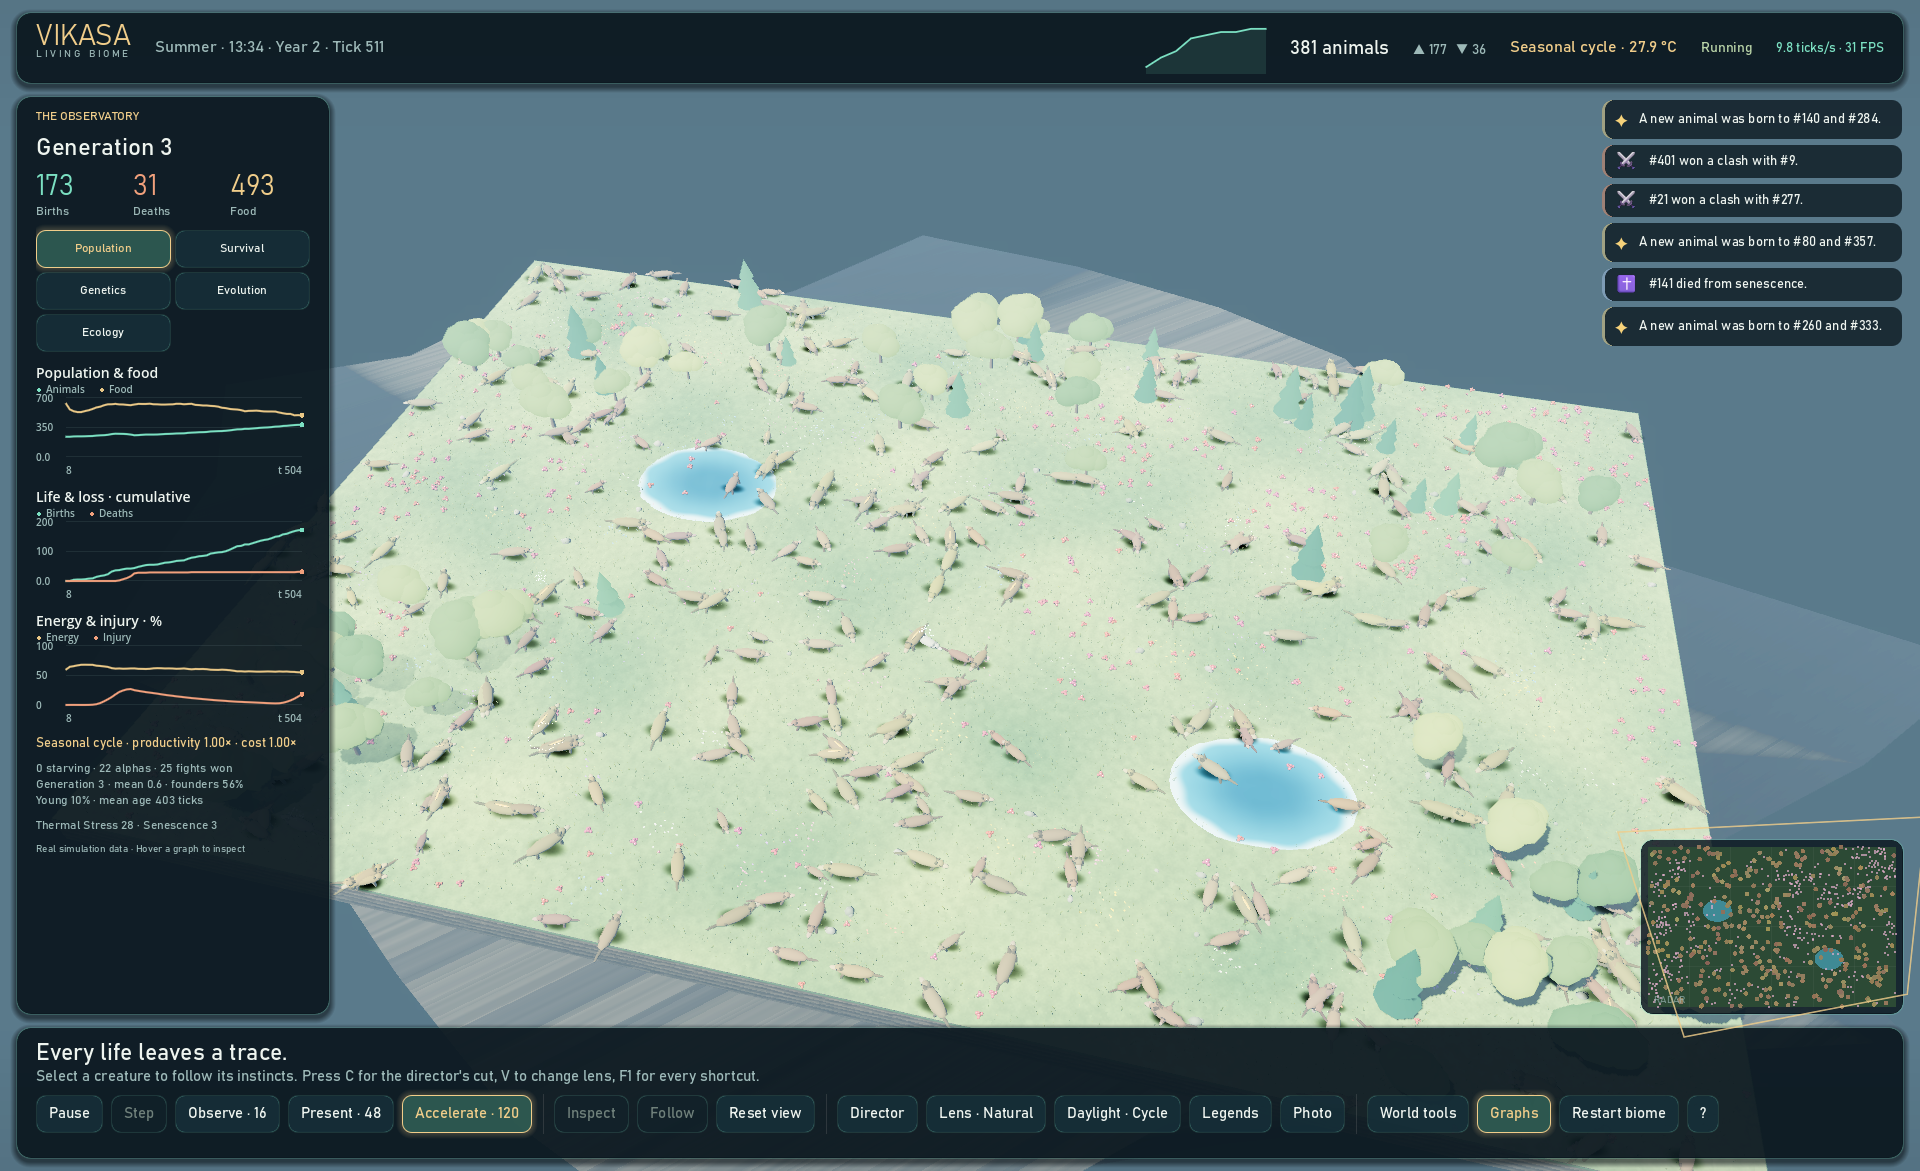
\includegraphics[width=0.55\textwidth]{climate-hud.png}
\caption{Warming demo with live temperature readout.}
\end{figure}

When the estimate and the live check disagree, the live check is the answer. For a
six-year locally adapted species in Hyderabad under SSP5-8.5 the estimate is 58\%
(narrow reference organism) while the live check gives 4 of 4 survivors; the app
shows both and says which to trust.

%===========================================================
\chapter{Conservation Planner}
\label{ch:planner}
%===========================================================

\section{Purpose}
Conservation teams work from a watchlist and a fixed budget. The planner answers
which species to act on first, by when and how, from Vikasa's measured rescue
results. It is a screening tool for prioritising field work, not a substitute for it.

\begin{figure}[htbp]
\centering
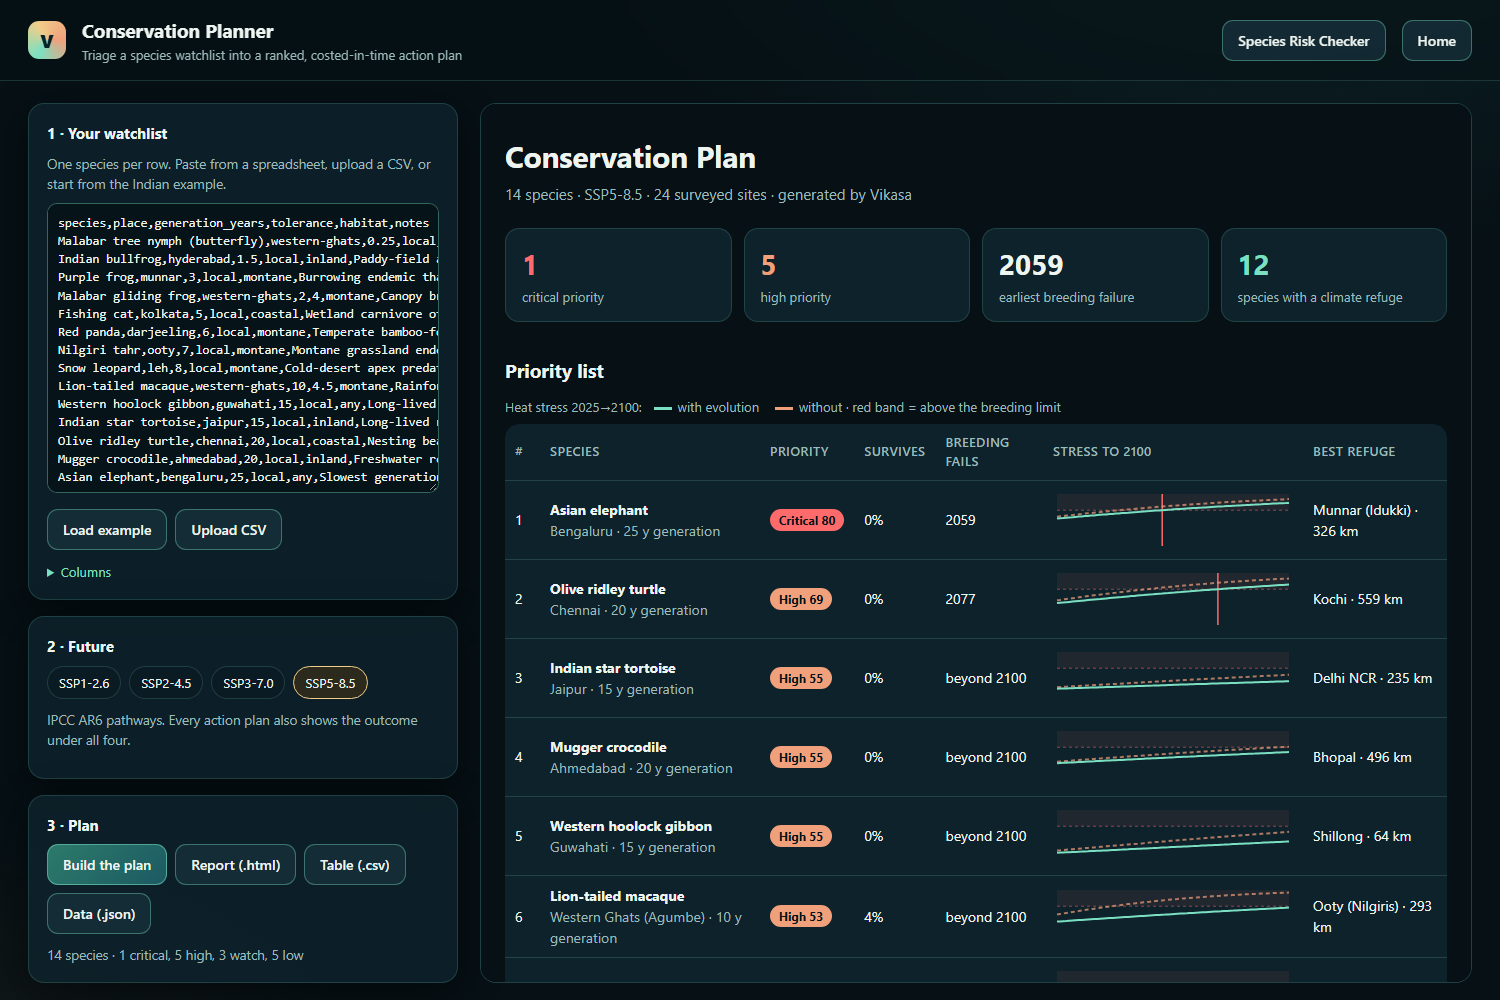
\includegraphics[width=0.85\textwidth]{conservation-planner.png}
\caption{Conservation Planner browser app with the Indian example watchlist.}
\end{figure}

\section{The adaptation-lag model}
For each year $y=2025,\dots,2100$:
\begin{enumerate}[leftmargin=*]
\item Climate is the place's monthly climatology plus the SSP anomaly for $y$.
\item With evolution, the optimum follows warming at the tracking rate
$\min(\dot T_{\text{SSP}},\,k_c/G_{\text{yr}})$, i.e.\ $\theta(y)=\bar T+\text{track}\cdot\max(0,y-2005)$;
without evolution it stays at $\bar T$.
\item Worst-month stress uses the asymmetric rule (warm side $0.6\omega$).
\item Breeding fails in the first year stress exceeds $0.75$ (breeding limit 0.7
plus the 0.05 borderline band), so a borderline place is not reported as failing in 2025.
\end{enumerate}

\section{Interventions}
\textbf{Assisted gene flow.} If no help is needed the shift is 0. Otherwise a grid
in 0.25\,$^{\circ}$C steps up to 15\,$^{\circ}$C finds the first sufficient shift,
then 18 bisection steps refine it, and the answer is rounded \emph{up} to 0.01 so a
reported shift never falls short. \code{None} means no shift works because the
seasonal swing is too wide for the tolerance. Donor sites are places 0--4\,$^{\circ}$C
warmer than home plus the needed shift.

\textbf{Refuges.} Translocated stock keeps its home optimum and is conservatively
not credited with adapting to the new site. A site is a \emph{refuge} if stress
stays under the failure line every year 2030--2100, a \emph{future refuge} if too
cold today but suitable by 2100, and otherwise unsuitable. The optional habitat
(\code{coastal}, \code{montane}, \code{inland}, \code{any}) restricts candidate sites;
distances are great-circle kilometres.

\section{Priority and tiers}
\[
\text{priority}=100\Big(0.55\,(1-p_{\text{surv}})+0.45\cdot\mathrm{clip}\Big(\frac{2100-y_{\text{fail}}}{75}\Big)\Big),
\]
with urgency 0 if breeding never fails. Not viable today gives 100; failure by 2050
gives at least 70. Tiers: Critical $\ge70$, High $\ge45$, Watch $\ge20$, Low below.
The action list is rule-based: gene flow, migration, protecting microrefugia and
corridors, and, when the survival curve and the timeline disagree, ``Confirm with
the live simulation'' first.

\section{Watchlist format and outputs}
CSV columns: \code{species}, \code{place}, \code{generation\_years} (required);
\code{tolerance}, \code{habitat}, \code{ssp}, \code{notes} (optional). Up to 200 rows;
bad rows are reported and skipped. \code{vikasa plan triage} writes a
self-contained \code{report.html} (no scripts, no network, prints cleanly),
\code{plan.csv} and \code{plan.json} (schema \code{vikasa-conservation-plan-v1}).
Twenty-four NASA POWER sites are searched: the seven cities, three study regions
and fourteen survey sites (Ooty, Munnar, Kochi, Pune, Nagpur, Bhopal, Ahmedabad,
Lucknow, Guwahati, Shillong, Darjeeling, Dehradun, Srinagar, Leh).

{\small
\begin{longtable}{clllcl}
\caption{Example triage, \code{examples/watchlist-india.csv}, SSP5-8.5 (illustrative generation times)}\\
\toprule
\# & Species & Place & Tier & Score & First action \\
\midrule
\endfirsthead
\toprule
\# & Species & Place & Tier & Score & First action \\
\midrule
\endhead
1 & Asian elephant & Bengaluru & Critical & 80 & Gene flow +1.3\,$^{\circ}$C \\
2 & Olive ridley turtle & Chennai & High & 69 & Gene flow +0.66\,$^{\circ}$C \\
3 & Indian star tortoise & Jaipur & High & 55 & Confirm with live simulation \\
4 & Mugger crocodile & Ahmedabad & High & 55 & Confirm with live simulation \\
5 & Western hoolock gibbon & Guwahati & High & 55 & Confirm with live simulation \\
6 & Lion-tailed macaque & Western Ghats & High & 53 & Confirm with live simulation \\
7 & Snow leopard & Leh & Watch & 44 & Confirm with live simulation \\
8 & Nilgiri tahr & Ooty & Watch & 35 & Confirm with live simulation \\
9 & Red panda & Darjeeling & Watch & 23 & Protect microrefugia \\
10 & Fishing cat & Kolkata & Low & 13 & Protect microrefugia \\
11 & Purple frog & Munnar & Low & 3 & Routine monitoring \\
12 & Indian bullfrog & Hyderabad & Low & 1 & Run the live check \\
13 & Malabar gliding frog & Western Ghats & Low & 1 & Routine monitoring \\
14 & Malabar tree nymph & Western Ghats & Low & 0 & Routine monitoring \\
\bottomrule
\end{longtable}}

For the elephant, breeding fails in 2059 with evolution and 2046 without, and the
best refuge is Munnar (326\,km); for the olive ridley, 2077 versus 2054, refuge
Kochi (559\,km).

\begin{figure}[htbp]
\centering
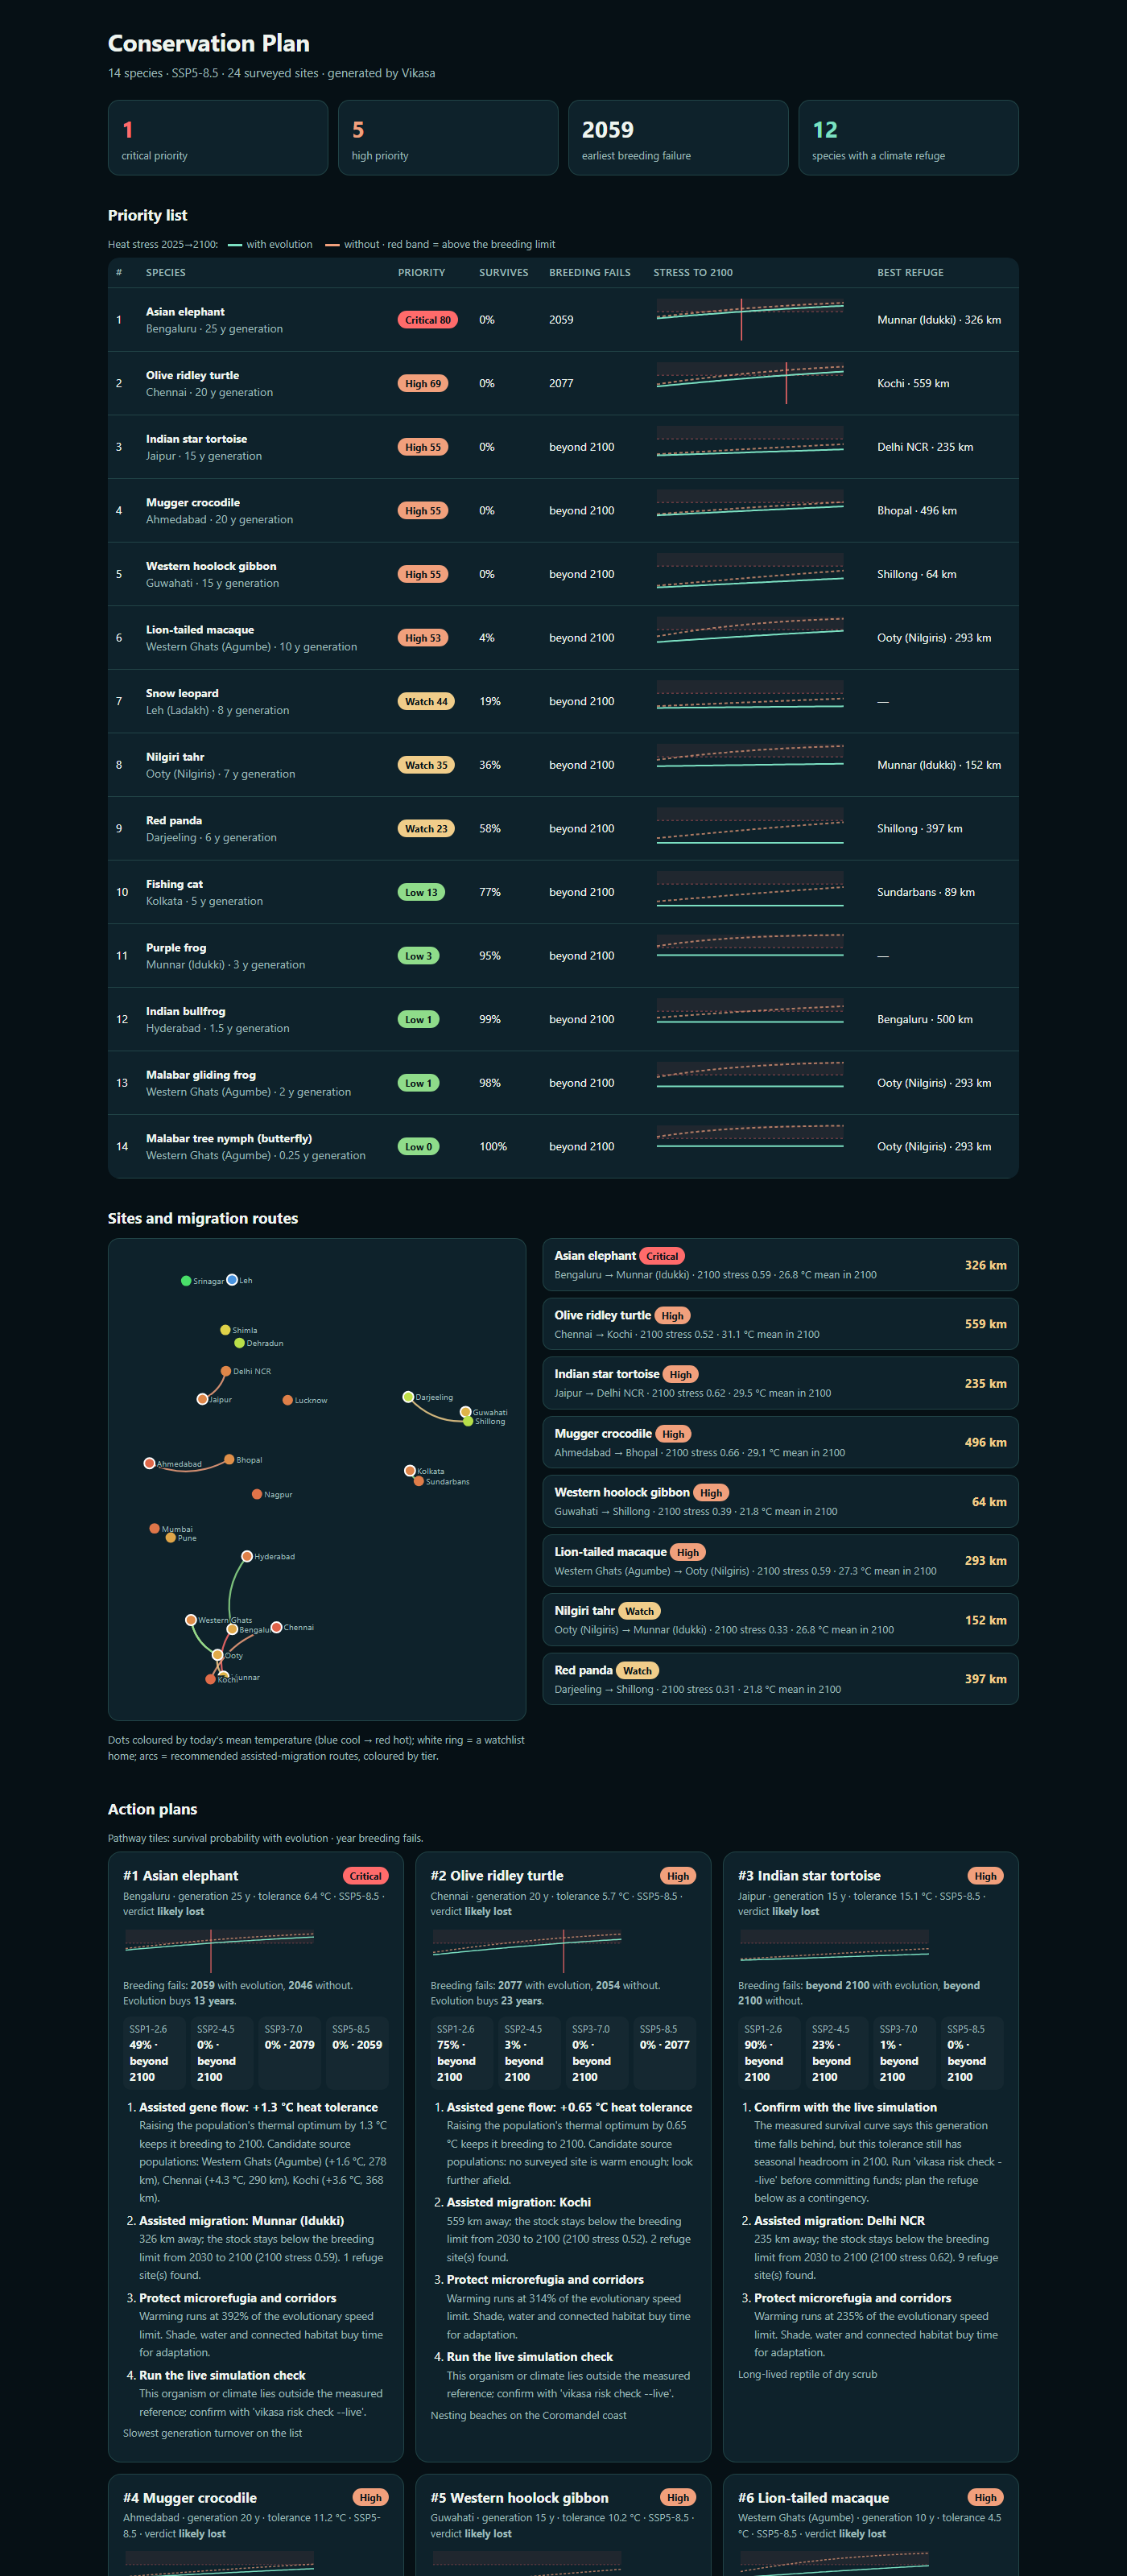
\includegraphics[height=0.42\textheight]{conservation-report.png}
\caption{Self-contained conservation plan report: priority list, migration routes and action cards.}
\end{figure}

%===========================================================
\chapter{Persistence and Checkpoints}
%===========================================================

\section{Format}
Checkpoints are JSON documents with format \code{vikasa}, \textbf{version 3}. They
store the resolved configuration, seed, tick, the NumPy PCG64 bit-generator state,
all creatures (genome, haplotypes, temperament, energy, injury, age, starvation
counter, current action, drives, utilities, targets, home-range and migration
state, satisfaction components, alpha status, belief, and with climate forcing the
thermal optimum and stress), resources, lineage, the environment and event
history, the culture ledger, metrics (including the last 512 birth cohorts), the
optional habitat grids and ledgers, intervention records, cumulative counters and
the fractional food-spawn accumulator.

\section{Atomic saving}
\code{save\_checkpoint} serialises the payload, rejects non-finite values (NaN or
infinity are refused rather than written as invalid JSON), writes a temporary
sibling file, flushes and syncs it, and atomically replaces the destination. An
interrupted save therefore never leaves a half-written checkpoint.

\section{Loading, migration and validation}
\code{load\_checkpoint} accepts versions 1, 2 and 3. Versions 1 and 2 are migrated
in memory: missing behaviour and home-range fields receive defaults, and
home radii are sampled deterministically per creature. Loading never rewrites the
source file; saving a migrated run writes version 3. Version 3 is strict:
required fields must be present, IDs and references must be JSON integers (booleans
and floats are rejected), and invariants must hold. The loader rejects malformed
habitat grids, impossible initialisation totals, unadvanced dynamic fluxes,
unbalanced reservoir ledgers, persisted birth histories that are out of order or
violate the Price identity, and unsupported versions. All failures raise
\code{CheckpointError} and fail closed.

\section{Continuation guarantee}
Because the RNG state and spawn accumulator are stored, a run saved at tick $t$
and resumed reproduces the same trajectory as an uninterrupted run on the same
software and numerical platform. The test suite checks this bit-for-bit.

%===========================================================
\chapter{The Simulation Bridge}
%===========================================================

\section{Role}
\code{bridge.py} serves the engine to the Godot client over a loopback-only HTTP
server (default port 8765; requests larger than 32\,KB are refused). The engine
advances in a background thread at the requested tick rate. Publication of the
binary frame (every 0.033\,s) and the explanation document (every 0.4\,s) happens
once per interval, so any number of readers share one serialisation.

\begin{table}[htbp]
\centering
\caption{Bridge endpoints}
\begin{tabularx}{\textwidth}{llL}
\toprule
Method & Path & Purpose \\
\midrule
GET & \code{/health} & Liveness probe. \\
GET & \code{/stream} & Long-lived push of length-prefixed (\code{<I} byte count) float32 frames at up to 30\,Hz. \\
GET & \code{/frame} & The latest frame as one response (fallback). \\
GET & \code{/state?lite=1\&focus=ID\&hs=T\&bs=T} & Explanation document: compact fields for every animal, full detail for the focus, and only history/birth rows newer than the client cursors \code{hs}/\code{bs}. \\
POST & \code{/command} & JSON command; result published immediately. \\
\bottomrule
\end{tabularx}
\end{table}

\section{Binary frame layout (version 2)}
A frame is a flat little-endian float32 array: a 24-value header, then 18 values
per creature (sorted by ID), then 4 values per food patch.

\begin{longtable}{cl|cl}
\caption{Frame header (24 float32 values)}\\
\toprule
Index & Field & Index & Field \\
\midrule
0 & frame version (2.0) & 12 & weather code ($-1$ none) \\
1 & tick & 13 & weather intensity \\
2 & creature count & 14 & weather remaining fraction \\
3 & resource count & 15 & world width \\
4 & creature stride (18) & 16 & world height \\
5 & resource stride (4) & 17 & total births \\
6 & paused flag & 18 & total deaths \\
7 & requested ticks/s & 19 & event-feed sequence \\
8 & measured ticks/s & 20 & food multiplier \\
9 & year phase $(\text{tick}\bmod384)/96$ & 21 & health pressure \\
10 & temperature index & 22 & maximum energy \\
11 & rainfall & 23 & reserved (0) \\
\bottomrule
\end{longtable}

\begin{longtable}{cl|cl}
\caption{Per-creature record (18 float32 values)}\\
\toprule
Offset & Field & Offset & Field \\
\midrule
0 & id & 9 & perception gene \\
1--2 & position $x,y$ & 10 & aggression \\
3--4 & velocity $v_x,v_y$ & 11 & resilience \\
5 & energy fraction $E/E_{\max}$ & 12 & sociability \\
6 & action code & 13 & flags bitmask \\
7 & size gene & 14 & dynasty (founder ID) \\
8 & speed gene & 15 & generation depth \\
 & & 16 & age (ticks) \\
 & & 17 & injury \\
\bottomrule
\end{longtable}

Flags: 1 alpha, 2 injured ($I>0.12$), 4 young (has parents and age below the
dependent age), 8 starving, 16 believer. Weather codes index the list drought,
abundance, heat, cold, storm, flood, wildfire, disease, redistribute; an import-time
check fails if this list ever diverges from the engine's event kinds. Each food
record is (id, $x$, $y$, energy).

\section{Commands}
\begin{table}[htbp]
\centering
\caption{\code{POST /command} actions}
\begin{tabularx}{\textwidth}{lL}
\toprule
Action & Effect \\
\midrule
\code{pause} / \code{resume} & Stop or continue ticking. \\
\code{speed} & Set requested ticks per second (Observe 16, Present 48, Accelerate 120). \\
\code{step} & Advance one tick while paused. \\
\code{weather} & Schedule an event with kind, intensity and duration from the current tick. \\
\code{food} & Add one audited external food patch at a position. \\
\code{food\_burst} & Scatter up to 24 audited patches on a spiral (the UI uses 10). \\
\code{restart} & Rebuild the world with the same configuration and seed, clearing histories. \\
\bottomrule
\end{tabularx}
\end{table}

\section{Event feed}
Per-tick births, deaths, clashes and culture entries enter a sequenced feed of the
last 240 entries. The frame header carries the latest sequence number, so the
client requests only missed entries and nothing is lost between polls. The bridge
also reports the host power source, which the client uses to adapt frame pacing on
battery.

%===========================================================
\chapter{The Godot Living Biome Client}
%===========================================================

\section{Scripts}
\begin{longtable}{p{4.2cm}p{10.8cm}}
\caption{Godot client scripts (\code{godot/scripts/})}\\
\toprule
Script & Role \\
\midrule
\endfirsthead
\toprule
Script & Role \\
\midrule
\endhead
\code{Main.gd} & Scene root: wiring, keyboard shortcuts, director mode, lenses, photo mode, extinction reseed in director mode. \\
\code{SimulationClient.gd} & Non-blocking stream socket, frame decoding, worker-thread JSON parsing, command posting. \\
\code{CreatureMesh.gd} & Bakes one procedural quadruped whose vertices are tagged with body part and material region. \\
\code{CreatureSwarm.gd} & Near/far LOD \code{MultiMesh} draws (up to 640 instances), interpolation, births, deaths, picking. \\
\code{WorldView.gd} & Selection halo, sensing and home-range rings, target lines, kin threads. \\
\code{Habitat.gd}, \code{HabitatMap.gd} & Terrain, 26{,}000 instanced grass blades, flowers, trees, water, cliff island; ecology cell map. \\
\code{Atmos.gd}, \code{AtmosphereOverlay.gd} & Sky, sun/moon, daylight cycle, seasons tint; screen-space vignette. \\
\code{WeatherFX.gd}, \code{LifeFX.gd}, \code{FoodField.gd} & GPU weather particles; birth/death/clash/crowning/bloom particles; instanced glowberry food. \\
\code{HUD.gd}, \code{UITheme.gd} & Top bar (tick rates, season, $^{\circ}$C, lag tooltip), panels and theme. \\
\code{CreatureInspector.gd}, \code{BehaviorPresentation.gd} & Profile with drives, utilities, genes, lineage; readable action presentation. \\
\code{Observatory.gd}, \code{LiveChart.gd}, \code{LocusChart.gd} & Chart groups, bounded histories with hover, chromosome charts. \\
\code{EventFeed.gd}, \code{Minimap.gd}, \code{LegendsPanel.gd} & Live feed, radar, hall of legends. \\
\code{CameraRig.gd}, \code{CinematicLayer.gd} & Orbit/pan/zoom camera; letterbox and captions. \\
\code{WorldTools.gd}, \code{Overlays.gd}, \code{ViewModes.gd} & Weather and food tools; overlays; lens definitions. \\
\code{QualityManager.gd}, \code{PerfOverlay.gd} & Adaptive quality tiers; F3 frame-time graph. \\
\code{Soundscape.gd} & Procedurally synthesised wind, rain, birds, crickets, thunder and chimes. \\
\code{DemoPilot.gd}, \code{HelpOverlay.gd} & Narrated autopilot; F1 field guide. \\
\code{MeshMerge.gd} & Mesh merging helper for static scenery. \\
\bottomrule
\end{longtable}

Shaders in \code{godot/shaders/}: \code{creature}, \code{grass}, \code{terrain},
\code{water}, \code{sky}, \code{weather} and \code{life\_fx}.

\section{Rendering pipeline}
The population costs two draw calls: one baked quadruped mesh drawn as near and
far \code{MultiMesh} LODs, plus a third for soft contact shadows. The vertex shader
animates gait, lying down, head dips, idle glances and tail wags, and expresses
genes as ears, ridges and tail length; the fragment shader shades hide, underside,
eyes and the alpha mantle. Previously each animal was 20--60 scene nodes and a
frame cost about 2{,}300 draw calls. Vegetation, food and particles are also
instanced and GPU-animated; particle timing lives in float32 transforms because the
Compatibility renderer stores MultiMesh custom data at half precision. Lighting
uses a texture-free sky shader, colour ambient light, ACES tone mapping, glow, fog
and one shadowed sun/moon with a 2048 orthogonal shadow map, with shadow casting
limited to trees.

\section{Adaptive quality}
\begin{table}[htbp]
\centering
\caption{Quality tiers}
\begin{tabular}{lcccccc}
\toprule
Tier & Render scale & MSAA & Glow & Shadows & Grass & LOD distance \\
\midrule
battery & 72\% & off & off & off & 35\% & 26 \\
balanced & 85\% & off & on & on & 60\% & 36 \\
high & 100\% & 2$\times$ & on & on & 85\% & 48 \\
ultra & 100\% & 4$\times$ & on & on & 100\% & 72 \\
\bottomrule
\end{tabular}
\end{table}
\code{auto} starts at \emph{high}, steps down after two consecutive windows in
which 10\% of frames exceed 23.5\,ms, and climbs back after 20\,s of headroom. F4
cycles auto/battery/balanced/high/ultra and persists the choice; FXAA is always on.
On battery, if the lowest tier still misses frames, the client switches to unlocked
pacing and restores vsync on mains power.

\section{Controls}
\begin{table}[htbp]
\centering
\caption{Living Biome controls}
\begin{tabularx}{\textwidth}{lL}
\toprule
Key / mouse & Action \\
\midrule
Space $\cdot$ 1 $\cdot$ 2 $\cdot$ 3 & Pause/resume $\cdot$ Observe 16 $\cdot$ Present 48 $\cdot$ Accelerate 120 ticks/s \\
Right-drag $\cdot$ middle-drag/WASD $\cdot$ Q/E $\cdot$ wheel & Orbit $\cdot$ pan $\cdot$ rotate $\cdot$ zoom \\
Click $\cdot$ double-click $\cdot$ Tab $\cdot$ F & Select and explain $\cdot$ fly to and follow $\cdot$ next animal $\cdot$ follow \\
C $\cdot$ V $\cdot$ N $\cdot$ L & Director $\cdot$ lens $\cdot$ daylight $\cdot$ legends \\
G $\cdot$ T $\cdot$ M $\cdot$ H $\cdot$ P & Graphs $\cdot$ world tools $\cdot$ radar $\cdot$ hide interface $\cdot$ photo mode \\
F12 $\cdot$ K $\cdot$ F3 $\cdot$ F4 $\cdot$ F1 $\cdot$ Esc & Screenshot $\cdot$ sound $\cdot$ performance $\cdot$ quality $\cdot$ field guide $\cdot$ close \\
\bottomrule
\end{tabularx}
\end{table}

\begin{figure}[htbp]
\centering
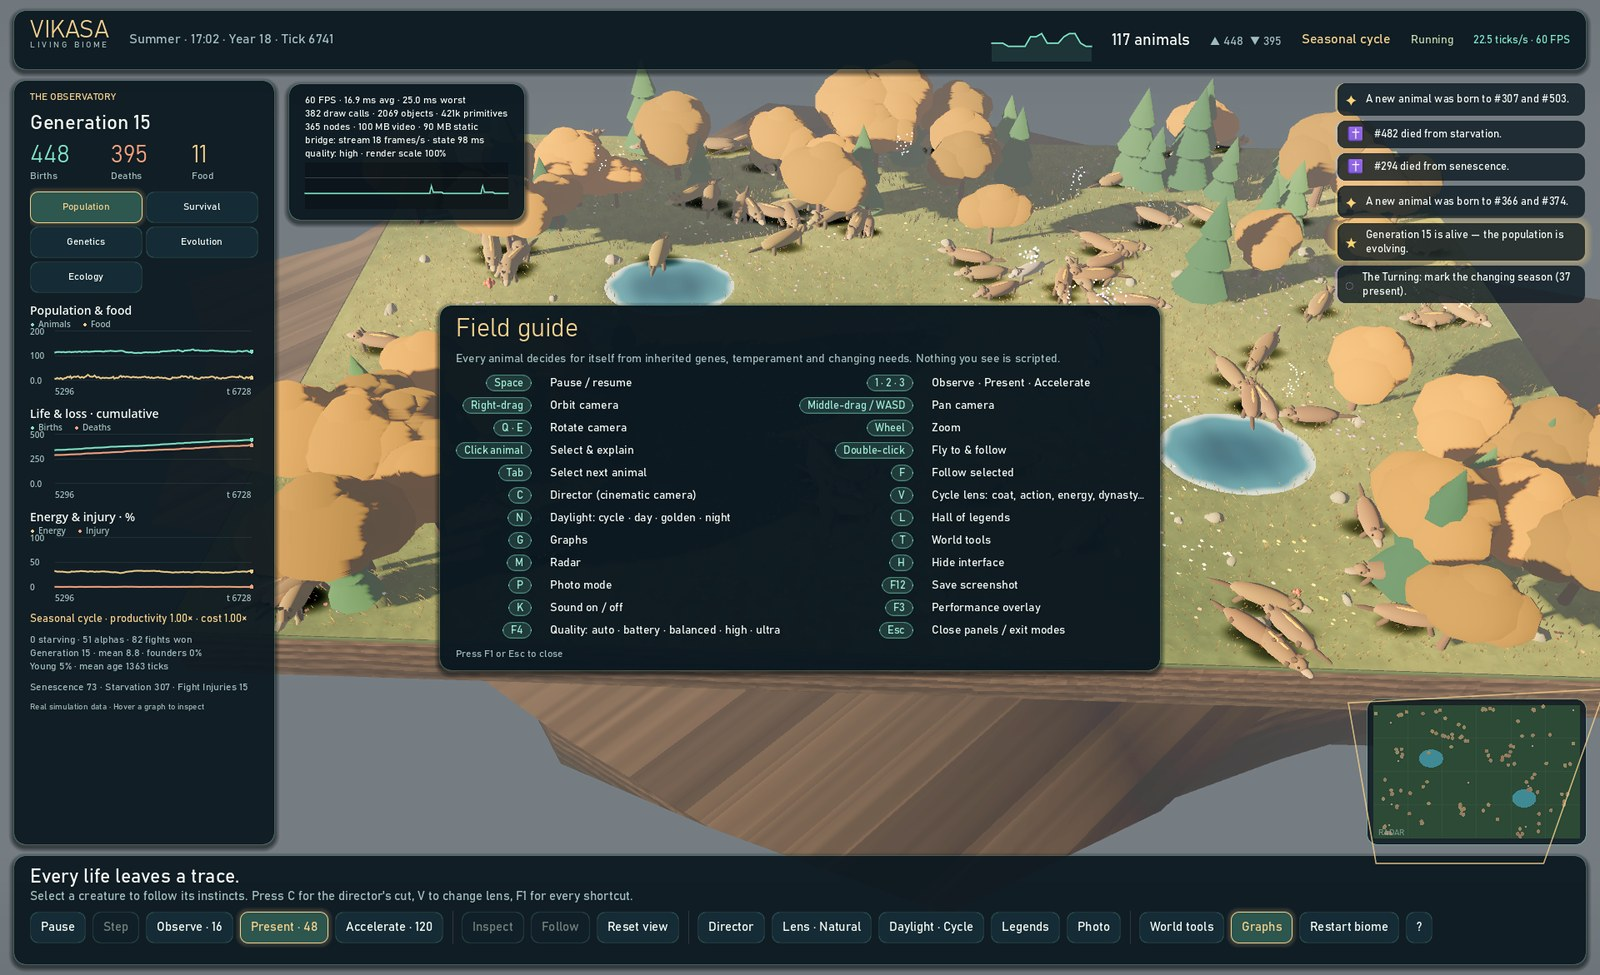
\includegraphics[width=0.6\textwidth]{showcase-help.jpg}
\caption{Field guide (F1) and the F3 performance overlay.}
\end{figure}

%===========================================================
\chapter{Local Application Server and API}
%===========================================================
\code{vikasa app}, \code{risk}, \code{plan} and \code{demo} serve one loopback
application on \code{http://127.0.0.1:8787}. The server refuses non-JSON and
cross-origin requests, and launch requests are whitelisted.

\begin{longtable}{p{2.1cm}p{5.4cm}p{6.9cm}}
\caption{Application server routes}\\
\toprule
Method & Path & Purpose \\
\midrule
\endfirsthead
GET & \code{/}, \code{/risk}, \code{/plan}, \code{/demo} & Home screen, Risk Checker, Planner, presenter hub. \\
GET & \code{/api/meta} & Places, presets, tolerance modes, SSPs, reference curve. \\
GET & \code{/api/estimate} & Instant estimate (\code{place}, \code{generation\_years}, \code{tolerance}, \code{ssp}). \\
POST/GET & \code{/api/live}, \code{/api/live/<id>} & Start and poll a live check. \\
GET/POST & \code{/api/plan/example}, \code{/api/plan} & Example watchlist; triage a pasted or uploaded CSV. \\
POST & \code{/api/watch} & Write a scenario world and open it in 3D. \\
POST & \code{/api/launch} & Launch \code{biome}, \code{biome-demo} or \code{climate-demo}. \\
GET/POST & \code{/api/godot}, \code{/api/stop-godot} & 3D window status; close it. \\
POST & \code{/api/fetch} & Download a new place from NASA POWER. \\
GET & \code{/api/stats}, \code{/api/version} & Live project statistics; version handshake. \\
GET & \code{/evidence/...} & The committed evidence report. \\
POST & \code{/api/quit} & Shut down every Vikasa process. \\
\bottomrule
\end{longtable}

%===========================================================
\chapter{Testing and Quality Assurance}
%===========================================================

\section{Test suite}
\code{pytest} collects 554 tests (with \code{--strict-markers --strict-config};
long stress tests are marked \code{slow}). Hypothesis is available in the
development extras for property-based testing.

\begin{longtable}{p{4.4cm}p{10.6cm}}
\caption{Test areas}\\
\toprule
Area & What is verified \\
\midrule
\endfirsthead
\code{tests/model/} & Genome bounds and immutability, crossover/mutation, diploid expression and meiosis, entities, spatial hash, 2D maths. \\
\code{tests/simulation/} & Engine tick order and invariants, reproducibility of identical seeds, behaviour drives/utilities/arbitration, Gompertz demography, habitat growth, diffusion conservation and ledgers. \\
\code{tests/analytics/} & Metrics, exact Price identities, evolutionary change, trait-space PCA and undefined cases. \\
\code{tests/io/} & Checkpoint round-trips, migration, strict rejection of corrupted data; export manifests. \\
\code{tests/experiments/} & Runner, contrast protocol validation, paired statistics, dashboard. \\
\code{tests/climate/} & Data parsing and provenance, forcing, engine coupling, protocol, analysis, Sobol on Ishigami, surrogate, assessment, report, CLI, risk screen (published verdicts), planner. \\
\code{tests/ui/}, \code{test\_bridge\_stream.py} & Pygame smoke tests; binary frame contract and stream. \\
\code{test\_cli.py}, \code{test\_config.py}, \code{test\_shortcut.py}, \code{test\_documentation.py} & CLI parsing, configuration validation, shortcut creation; documented scenarios load, every documented mode is in the CLI help, example results are audited, screenshots are real rendered images. \\
\bottomrule
\end{longtable}

\section{Godot headless checks}
\code{SceneContractSmoke}, \code{BehaviorPresentationSmoke}, \code{LocusChartSmoke}
and \code{DemoPilotSmoke} run headless. \code{PerfProbe} measures mean and p99 frame
time, slow-frame share, draw calls, node count and tier, with \code{--breakdown},
\code{--freeze}, \code{--no-state} and \code{--no-frames} isolation flags.
\code{ShowcaseCapture}, \code{PresentationCapture}, \code{WildlifeCapture} and
\code{MainCapture} regenerate documentation screenshots from real bridge states.

\section{Invariants}
\code{SimulationEngine.audit\_invariants} returns a list of violations, checked by
\code{stress}, \code{study}, \code{contrast} and the climate runs. It verifies that
dictionary keys match creature and resource IDs; motion state, energy and resource
state are finite; every creature lies inside the world; home centres, radii and
migration counters are valid; all six traits lie within configured bounds; diploid
genotypes are valid, require a diploid architecture and match the expressed
phenotype; thermal optima are valid and exist only with climate forcing; external
food inputs and their intervention history are finite and consistent; and the
habitat's update count equals the engine tick. Study reports additionally check
the population identity living $=$ founders $+$ births $-$ deaths, and checkpoint
loading verifies reservoir ledgers and Price identities.

%===========================================================
\chapter{Performance}
%===========================================================

\section{3D client}
Measured on an Intel Core i5-1335U with Iris Xe graphics, $1920\times1200$ at
59\,Hz, Windows 11, Godot 4 Compatibility renderer, showcase seed 2026 with about
110--170 animals.

\begin{table}[htbp]
\centering
\caption{Living Biome before and after version 2.0}
\begin{tabularx}{\textwidth}{lLL}
\toprule
Measure & Before (v1.1) & After (v2.0) \\
\midrule
Frame rate with vsync & 13--14 FPS & \textbf{59.6--59.9 FPS} at high \\
Uncapped, full interface & 35--152 FPS, p99 36--157 ms & 98--105 FPS high; 149 FPS balanced \\
Frames over 25 ms (vsync) & --- & 0.1--0.4\% (p99 21--22 ms, plugged in) \\
Draw calls / scene nodes & $\sim$1{,}700--2{,}450 / $\sim$3{,}000--3{,}600 & $\sim$20 for the 3D world ($\sim$300 with UI) / 365 \\
Explanatory document & 180--680 KB every 0.16--0.45 s & $\sim$35 KB every 0.4 s \\
State request latency & 49 ms median & 12 ms median \\
\bottomrule
\end{tabularx}
\end{table}

On battery, vsync'd rendering was near 45 FPS; after the battery-aware pacing
change \code{auto} settled on balanced, unlocked, at 94.5 FPS (p99 29\,ms). With the
complete 3D window open, this laptop sustained about 43 ticks/s in a 12-second
Accelerate sample; the 120 ticks/s setting is a ceiling, not a guarantee.

\section{Engine}
A profile of spatial-biome seed 2026 (150 ticks after 150 warm-up) attributed
2.54\,s to spatial rebuilding, 2.42\,s to insertion and 1.81\,s to radius queries
out of 13.72 profiled seconds. The spatial hash was then changed to validate each
position cloud with one NumPy reduction and keep copied scalar coordinates.
\code{tools/benchmark\_spatial.py} loads the historical index from Git into an
isolated namespace, alternates run order, and requires identical full checkpoint
digests at both boundaries.

\begin{table}[htbp]
\centering
\caption{Guarded spatial-index benchmark (Python 3.12.14, NumPy 2.5.3)}
\begin{tabular}{lccc}
\toprule
Seed & Historical ticks/s & Optimised ticks/s & Ratio \\
\midrule
2026 & 20.03 & 23.97 & 1.197 \\
7 & 21.72 & 24.94 & 1.148 \\
41 & 20.85 & 23.83 & 1.143 \\
\bottomrule
\end{tabular}
\end{table}
All pairs matched digests and reported no invariant errors: a local 14--20\%
improvement with unchanged biology, not a universal guarantee.

%===========================================================
\chapter{Command-Line Reference}
%===========================================================
All commands accept \code{--help}. Defaults shown are those in the parser.

\begin{longtable}{p{5.2cm}p{9.8cm}}
\caption{\code{vikasa} sub-commands and options}\\
\toprule
Command & Options and behaviour \\
\midrule
\endfirsthead
\toprule
Command & Options and behaviour \\
\midrule
\endhead
\code{app} & Home screen. \code{--port 8787}, \code{--no-browser}. \\
\code{demo} & Presenter hub. \code{--biome-only} (3D autopilot only), \code{--godot-path}, \code{--port}, \code{--no-browser}. \\
\code{risk} & Risk Checker app. \code{--port}, \code{--no-browser}. \\
\code{risk check} & Terminal verdict. \code{--place hyderabad}, \code{--generation-years 1.0}, \code{--tolerance local}, \code{--ssp SSP5-8.5}, \code{--live}, \code{--seeds 4}, \code{--json}. \\
\code{risk places} & List bundled places. \\
\code{plan} & Planner app. \code{--port}, \code{--no-browser}. \\
\code{plan triage WATCHLIST} & \code{--ssp SSP5-8.5}, \code{--output exports/plan}, \code{--open}. \\
\code{plan species} & \code{--name}, \code{--place}, \code{--generation-years}, \code{--tolerance}, \code{--habitat any}, \code{--ssp}, \code{--json}. \\
\code{godot} & 3D client with bridge. \code{--config config/showcase.json}, \code{--seed 2026}, \code{--godot-path}, \code{--demo}. \\
\code{serve} & Bridge only. \code{--config}, \code{--seed 2026}, \code{--port 8765}. \\
\code{validate} & \code{--config} (required). \\
\code{run} & \code{--scenario}, \code{--output} (required), \code{--ticks}, \code{--seed}. \\
\code{batch} & \code{--scenario}, \code{--output}, \code{--replicates 3}, \code{--ticks}. \\
\code{study} & \code{--config}, \code{--seeds 2026 7 41}, \code{--ticks 12000}, \code{--sample-interval 500}, \code{--output}. \\
\code{contrast} & \code{--protocol}, \code{--output} (new directory). \\
\code{stress} & \code{--config}, \code{--ticks 100000}, \code{--seed 2026}. \\
\code{shortcut} & \code{--desktop}, \code{--name Vikasa}, \code{--only app|biome|demo|risk}, \code{--config}, \code{--seed}. \\
\code{climate pipeline} & \code{--profile quick|full}, \code{--root}; resumable. \\
\code{climate fetch} & \code{--lat}, \code{--lon}, \code{--name}, \code{--key}, \code{--output}. \\
\code{climate assess} & \code{--root}, \code{--region}, \code{--generation-years}, \code{--breadth}, repeated \code{--ssp}. \\
\code{climate report} & \code{--root}; writes the offline HTML report and manifest. \\
\bottomrule
\end{longtable}

%===========================================================
\chapter{Reproducing the Evidence}
%===========================================================
Every committed result can be regenerated. Use a fresh output directory each
time; keep reports with their source and configuration versions.

\begin{lstlisting}
# Climate rescue (full profile, resumable)
vikasa climate pipeline --profile full --root exports\climate\full

# Showcase development study and extinction control
python -m evolution_sim.cli study --config config/showcase.json --seeds 2026 7 41 --ticks 12000 --output exports/development-study.json
python -m evolution_sim.cli study --config config/extinction-control.json --seeds 2026 7 41 --ticks 12000 --output exports/extinction-control-study.json

# Spatial ecology, 6,000 ticks
python -m evolution_sim.cli study --config config/spatial-biome.json --seeds 2026 7 41 --ticks 6000 --sample-interval 500 --output exports/spatial-biome-study-6000.json

# Weather laboratory preview and the larger prospective protocol
python -m evolution_sim.cli contrast --protocol experiments/weather-contrast-preview.json --output exports/weather-preview
python -m evolution_sim.cli contrast --protocol experiments/weather-contrast.json --output exports/weather-study

# Trait geometry snapshot
vikasa run --scenario experiments\baseline.json --output exports\trait-snapshot --seed 2026 --ticks 800

# Spatial-index benchmark with digest equality
python tools\benchmark_spatial.py --config config\spatial-biome.json --baseline 5874e01 --seeds 2026 7 41 --warmup 150 --ticks 300 --output exports\spatial-performance-new.json

# Conservation plan for the example watchlist
vikasa plan triage examples\watchlist-india.csv --open

# 3D performance probe (bridge on port 8766)
vikasa serve --config config\showcase.json --seed 2026 --port 8766
& $env:VIKASA_GODOT_BINARY --path godot --script res://tests/PerfProbe.gd -- --port 8766 --seconds 15 --tier 2
\end{lstlisting}

\begin{table}[htbp]
\centering
\caption{Committed evidence packages (\code{docs/results/})}
\begin{tabularx}{\textwidth}{lL}
\toprule
Package & Contents \\
\midrule
\code{climate-rescue-2026-10-18/} & Calibration, sweep summary, Sobol, assessments, validation, figures, offline report, manifest. \\
\code{conservation-plan-india/} & \code{report.html}, \code{plan.csv}, \code{plan.json}. \\
\code{development-study-2026-10-08.json} & Showcase 12{,}000-tick study, three seeds. \\
\code{extinction-control-study-2026-10-08.json} & Preserved extinction-prone configuration. \\
\code{spatial-biome-study-6000-2026-10-08.json} & Spatial profile, 6{,}000 ticks. \\
\code{weather-laboratory-2026-10-08/} & \code{report.json}, viewer, manifest. \\
\code{spatial-performance-2026-10-08.json} & Benchmark with checkpoint digests. \\
\code{diploid-preview-2026-10-08/} & Unreleased chromosome preview: config, summary, trait space. \\
\bottomrule
\end{tabularx}
\end{table}

%===========================================================
\chapter{Limitations and Roadmap}
%===========================================================

\section{Model limitations}
\begin{itemize}[leftmargin=*]
\item Ticks have no calibrated real-time meaning; space is two-dimensional even when
rendered in 3D.
\item No food web, sex differentiation, calibrated genetic drift, explicit disease
transmission, hydrology, learned language or validated real-species parameters.
\item Combat, starvation, inheritance, environment and culture are intentionally
simplified rules; plausible animation does not validate them.
\item Daylight, sound, terrain relief, trees, water and weather particles are
scenery: the model has seasons but no day/night, and none of these visuals affect
movement, perception or survival.
\item Climate: the organism is generic; no plasticity, behavioural
thermoregulation, migration or food-web effects; populations of tens of animals;
regional warming is the global AR6 median times a factor, not a downscaled
projection; reanalysis cells smooth mountains and coasts; the direct regional
assessment caps warming at 40 generations.
\item Decision tools: the instant estimate is anchored to one reference organism;
the live check uses 4 seeds and has wide intervals; example generation times are
illustrative; real translocation and gene flow need species-specific ecology,
disease screening, genetic compatibility checks and permits; rainfall, habitat loss
and species interactions are not modelled.
\end{itemize}

\section{Research status}
\begin{longtable}{p{3.2cm}p{5.6cm}p{6.2cm}}
\caption{Research dimensions: target and current state}\\
\toprule
Dimension & Required end state & Current evidence and gap \\
\midrule
\endfirsthead
Sustained development & Long-horizon replicated runs with turnover and transparent extinction risk & 6{,}000-tick regression and three 12{,}000-tick probes persist; larger predeclared seed sets and sensitivity analysis needed. \\
Mechanistic ecology & Spatial biomass, water/nutrients, local exposure, refuges, explicit disease & Optional plant/water field and audited interventions; nutrients, local hazards and contagion needed. \\
Quantitative genetics & Inspectable inheritance, covariance, trade-offs, plasticity, drift vs selection & Six traits, exact Price decomposition, PCA exports, diploid preview; multilocus release, causal tests and plasticity needed. \\
Behavioural development & Energy-budget lifecycle, learning, defensible social transmission & Fixed utility behaviour and care; learning needed. \\
Visualisation & Lineage exploration, life stages, heatmaps, comparisons & Generation and Price graphs, ecology map; deeper exploration needed. \\
Experiment laboratory & Replicates, ablations, sensitivity, uncertainty, portable packages & Seed-blocked protocols, paired uncertainty, packages; mechanism-isolating ablations and larger prospective studies needed. \\
Communication & Equations, assumptions, units, verified screenshots, reproducible results & This document, the IEEE paper and the Markdown references. \\
\bottomrule
\end{longtable}

\section{Roadmap}
\begin{enumerate}[leftmargin=*]
\item Calibrate the organism against real species' thermal-performance and
life-history data.
\item Add phenotypic plasticity and behavioural thermoregulation, then re-measure $k_c$.
\item Dispersal on heterogeneous landscapes linking the spatial ecology to climate.
\item Downscaled regional projections in place of global medians.
\item Execute the eight-seed weather protocol and larger predeclared climate sweeps.
\item Mechanism-isolating ablations (inheritance, sterility, injury, metabolic cost).
\item Release the diploid architecture after long-horizon validation.
\item Live checkpoint integration in the bridge so field studies survive upgrades.
\end{enumerate}

%===========================================================
\chapter*{Appendix A: Glossary}
\addcontentsline{toc}{chapter}{Appendix A: Glossary}
%===========================================================
\begin{longtable}{p{3.8cm}p{11.2cm}}
\toprule
Term & Meaning \\
\midrule
\endfirsthead
Tick & One discrete engine step; no fixed real-time meaning. \\
Founder & An animal present at tick 0 (generation 0). \\
Generation depth & One plus the deepest parent's depth. \\
Generation interval $G$ & Ticks per generation, measured as $1/$slope of mean living depth. \\
Drive & A normalised pressure in $[0,1]$ (survival, foraging, mating, care, danger, territory). \\
Utility & A bounded action score from drive affinities, rewards and costs. \\
Hysteresis & Keeping the current action while it stays within a margin of the best. \\
Alpha & A retained marker of contest victory; not a permanent rank. \\
Health pressure & Summed weather-driven exposure pressure that causes injury. \\
Thermal optimum $\theta$ & Temperature at which an animal performs best. \\
Tolerance breadth $\omega$ & Cold-side width of the thermal-performance curve. \\
Thermal stress $\varsigma$ & One minus performance; 0.3 injury onset, 0.7 breeding limit. \\
Critical rate $k_c$ & Warming per generation at which survival probability is 0.5. \\
Rescue gain & Heritable minus control critical rate. \\
Adaptation lag & Warming minus evolved shift of the mean optimum. \\
Rescue signature & A dip below 50\% of pre-warming size followed by recovery to $\ge80\%$. \\
Critical generation time & $k_c$ divided by warming per year. \\
SSP & Shared socio-economic pathway (IPCC AR6 emission scenario). \\
Price decomposition & Exact split of trait change into selection and transmission terms. \\
Participation ratio & $1/\sum f_k^2$: effective number of variance directions. \\
Wilson interval & Score interval for a binomial proportion. \\
Seed block & Matched replicate unit for paired treatment--control comparison. \\
Sobol index & Variance share of an output attributable to an input ($S_1$) or including interactions ($S_T$). \\
Surrogate & Gaussian-process emulator of simulation outcomes. \\
Refuge & Site whose stress stays below the failure line every year 2030--2100. \\
Assisted gene flow & Introducing heat-tolerant individuals to shift the mean optimum. \\
\bottomrule
\end{longtable}

%===========================================================
\chapter*{Appendix B: Repository Layout}
\addcontentsline{toc}{chapter}{Appendix B: Repository Layout}
%===========================================================
\begin{lstlisting}
vikasa/
  pyproject.toml          package metadata, dependencies, pytest config
  main.py                 convenience entry point
  config/                 world configurations (showcase, spatial, climate...)
  experiments/            scenarios and contrast protocols
  examples/               watchlist-india.csv
  src/evolution_sim/
    config.py cli.py bridge.py shortcut.py
    model/                genome, genetics, temperament, entities, lineage, spatial
    simulation/           engine, behavior, environment, culture, snapshots
    analytics/            metrics, trait_space
    experiments/          runner, scenarios, contrast, charts, dashboard
    io/                   checkpoints, export
    climate/              data, forcing, thermal, protocol, analysis, sensitivity,
                          surrogate, assess, figures, report, risk, risk_app,
                          planner, cli, data/*.json (24 sites + reference),
                          web/ (home, risk, plan, demo pages + vikasa.css)
    assets/               icons
  godot/                  project.godot, Main.tscn, scenes/, scripts/, shaders/, tests/
  tests/                  pytest suite (554 tests)
  tools/                  benchmark_spatial, build_city_regions,
                          build_survey_regions, build_icons
  docs/                   Markdown guides, images/, results/,
                          paper/ (IEEE paper), manual/ (this document)
  output/pdf/             historical Mathematics Guide (commit 0140311)
\end{lstlisting}

\section*{Related documents}
\begin{itemize}[leftmargin=*]
\item \code{docs/paper/Vikasa\_IEEE\_Paper.pdf}: the eight-page IEEE-format research paper.
\item \code{docs/MATHEMATICS.md}, \code{SCIENTIFIC\_MODEL.md}, \code{ARCHITECTURE.md}: current model references.
\item \code{docs/CLIMATE\_RESCUE.md}, \code{RISK\_CHECKER.md}, \code{CONSERVATION\_PLANNER.md}: climate module guides.
\item \code{docs/SPATIAL\_ECOLOGY.md}, \code{CONTROLLED\_EXPERIMENTS.md}, \code{TRAIT\_GEOMETRY.md}, \code{PERFORMANCE.md}, \code{SHOWCASE.md}, \code{RESEARCH\_STATUS.md}.
\item \code{output/pdf/Vikasa\_Mathematics\_Guide.pdf}: historical mathematics PDF documenting commit \code{0140311}; its older death rules do not describe today's showcase.
\end{itemize}


\end{document}
